\documentclass[12pt, a4paper]{article}
\usepackage{graphicx} % Required for inserting images
\usepackage[utf8]{inputenc}
\usepackage[spanish]{babel}
\usepackage{booktabs}
\usepackage{enumitem}
\usepackage{xcolor}
\usepackage{float}
\usepackage{indentfirst} % Fuerz la sangría en el primer párrafo de cada sección
\usepackage{hyperref} % Esto además hará que los links sean clickeables
\usepackage[T1]{fontenc}

% --- Paquetes de Diseño y Estética ---
\usepackage{geometry}
\geometry{top=2.5cm, bottom=2.5cm, left=2.5cm, right=2.5cm}
\usepackage{fancyhdr} % Encabezados y pies de página
\usepackage{titlesec} % Formato de títulos

\usepackage{amsmath, amsfonts, amssymb}
\usepackage{tabularx}
\usepackage{multirow}

% --- Paquetes de Gráficos ---
\usepackage{caption}
\usepackage{subcaption}



\usepackage{amssymb}
\usepackage{siunitx}        % unidades SI  \SI{220}{\volt}
\usepackage{pgfplots}       % gráficas (opcional)
\pgfplotsset{compat=1.18}


\begin{document}
%%%%%%%%%%%%%%%%%
%%%% PORTADA %%%%%
%%%%%%%%%%%%%%%%%%%

\begin{titlepage}
\thispagestyle{empty}	% Quito los encabezados en esta página

\begin{tikzpicture}[remember picture,overlay]
    \node[opacity=0.2,anchor=center] at (current page.center) 
        {
\includegraphics[width=0.9\paperwidth]{decoracion_b.png}};
\end{tikzpicture}

\begin{center}
    
\includegraphics[width=15cm]{unc_fcefyn_logo.png}
    \\[0.5cm]
    \LARGE Universidad Nacional de Córdoba\\[0.5cm] 
    \large Facultad de Ciencias Exactas, Físicas y Naturales \\[0.5cm] 
    \large Síntesis de Redes Activas (2025)
    \\[0.5cm]
    \large Laboratorio N°3 (Circuito 1): 
    \\[0.2cm]
    \large Diseño y compensación de amplificadores compuestos\\
    con tecnologías VFA y CFA
    \vspace{60pt}
    \begin{table}[!h]
    \centering
    \begin{tabular}{ll}
    \multicolumn{1}{l}{Alumnos:} & \multicolumn{1}{c}{DNI} \\
    Arteaga Barrera, Cristian Eduardo & 95.159.096 \\
    Baccino, Luca & 45.328.380 \\
    Baccino, Octavio & 44.350.820 

    \end{tabular}
    \end{table}
    \vspace{20pt}
    \begin{table}[!h]
    \centering
    \begin{tabular}{ll}
    \multicolumn{1}{c}{Docentes:} & Dr. Ing. Ferreyra Pablo \\
                         & Ing. César Reale
    \end{tabular}
    \end{table}
    \vfill
    Córdoba, República Argentina\\
    

\end{center}

\end{titlepage}
\tableofcontents
\newpage % Salto de página para que el texto empiece en la hoja siguiente
\newpage
\listoffigures
\newpage
\listoftables
\newpage

\section{Introducción}

    El presente informe detalla el diseño, análisis y simulación (mediante el programa LTSpice (x64)) de circuitos analógicos basados en amplificadores operacionales de dos tipologías distintas, el amplificador operacional realimentado por tensión (VFA) y el amplificador operacional realimentado por corriente (CFA). Para ello se propone un circuito de un amplificador compuesto (\autoref{fig:circuito_1}), con combinaciones VFA-VFA, VFA-CFA y un VFA-CFA con una red de compensación cero-polo.\\


Los amplificadores operacionales seleccionados para el diseño de los distintos circuitos son el LM324 (VFA) y el LM6181 (CFA) de los cuales se tienen las especificaciones detalladas en \autoref{tab:param_vfa} y \autoref{tab:param_cfa} respectivamente.

\begin{table}[htbp]
    \centering
    \caption{Parámetros dinámicos del amplificador VFA (LM324).}
    \label{tab:param_vfa}
    \begin{tabular}{@{}ll@{}}
        \toprule
        \textbf{Parámetro} & \textbf{Valor Nominal} \\
        \midrule
        Ganancia de lazo abierto ($Ad_0$) & \SI{100}{dB} \\
        Frecuencia de transición ($F_T$)  & \SI{1}{MHz} \\
        Frecuencia del primer polo ($F_1$) & \SI{10}{Hz} \\
        Frecuencia del segundo polo ($F_2$) & \SI{5,06}{MHz} \\
        \bottomrule
    \end{tabular}
\end{table}

\begin{table}[htbp]
    \centering
    \caption{Parámetros de transimpedancia del amplificador CFA (LM6181).}
    \label{tab:param_cfa}
    \begin{tabular}{@{}ll@{}}
        \toprule
        \textbf{Parámetro} & \textbf{Valor Nominal} \\
        \midrule
        Resistencia de transimpedancia ($R_T$) & \SI{2,37}{M\Omega} \\
        Capacitancia de transimpedancia ($C_T$) & \SI{4,8}{pF} \\
        Frecuencia del primer polo ($F_1$) & \SI{14}{kHz} \\
        Frecuencia del segundo polo ($F_2$) & \SI{82,3}{MHz} \\
        \bottomrule
    \end{tabular}
\end{table}

\subsection{Circuito: Amplificador compuesto}

\begin{figure}[http]
    \centering
    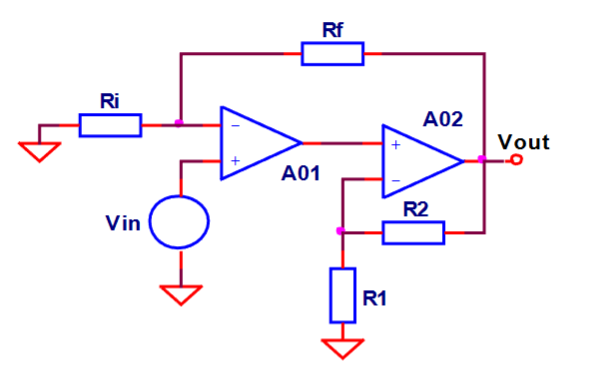
\includegraphics[width=0.5\linewidth]{Imagenes/circuito_1.png}
    \caption{Circuito 1: Amplificador compuesto}
    \label{fig:circuito_1}
\end{figure}

Para este circuito se busca un diseño que obtenga una \textbf{ganancia global} ($A_{vf}$) de 20 dB, compensándolo para obtener una \textbf{máxima planicidad de módulo}, es decir, un margen de fase ($M_\varphi$) de \ang{65} o, equivalentemente, un factor de calidad de los polos ($Q_p$) de $0{,}707$.

\subsection{Caso 1: VFA-VFA}
Como primer caso de estudio se propone utilizar dos amplificadores operacionales de la misma tipología (VFA-VFA) donde se busca:

\begin{enumerate}
    \item Diseñar el amplificador compuesto VFA+VFA
    \item Calcular el ancho de banda potencial.
    \item Determinar la frecuencia del polo de la función de transferencia a lazo cerrado.
    \item Determinar el ancho de banda real a -3dB.
    \item Medir el ancho de banda real
    \item Estimar el margen de fase obtenido en base a la respuesta al escalón.
\end{enumerate}

\subsection{Caso 2: VFA-CFA}
Como segundo caso se busca un circuito que combina las topologías VFA y CFA donde se busca:

\begin{enumerate}
    \item Diseñar el amplificador VFA-CFA para máxima planicidad de módulo y que además cumpla con el ancho de banda potencial aproximado de $f_g = 2\ MHz$
    \item Calcular el ancho de banda potencial
    \item Calcular la frecuencia del polo de la función de transferencia a lazo cerrado
    \item Calcular el ancho de banda real
    \item Medir el ancho de banda a 3 dB.
    \item Estimar el margen de fase obtenido en base a la respuesta al escalón.
\end{enumerate}

\subsection{Caso 3: VFA-CFA (Compensado)}
Como último caso se agrega una red de compensación \textbf{cero - polo} a la salida del VFA al circuito del caso 2. Se busca cancelar el segundo polo del VFA con el cero de la red de compensación y ubicar el polo de la misma por lo menos una octava después para no influir en el mismo. Se busca:

\begin{enumerate}
    \item Retocar la ganancia del CFA para contrarrestar la atenuación producida por la red de compensación.
    \item Calcular el ancho de banda potencial
    \item Calcular la frecuencia del polo de la función de transferencia a lazo cerrado
    \item Calcular el ancho de banda real
    \item Medir el ancho de banda a 3 dB.
    \item Constatar la mejora del margen de fase obtenido en base a la respuesta al escalón.
\end{enumerate}



\newpage

\section{Marco Teórico}

\subsection{Amplificadores Realimentados por Tensión (VFA)}

El Amplificador Operacional clásico, o Amplificador Realimentado por Tensión (VFA, por sus siglas en inglés), es un dispositivo fundamental en la electrónica analógica.

\subsubsection{Características Principales}
\begin{figure}[H]
    \centering
    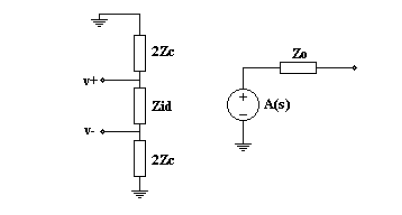
\includegraphics[width=0.5\linewidth,height=0.32\textheight,keepaspectratio]{Imagenes/modelo_VFA.png}
    \caption{Modelo real del VFA}
    \label{fig:modelo_VFA}
\end{figure}

El modelo en pequeña señal de un VFA, \autoref{fig:modelo_VFA}, se caracteriza por poseer una impedancia de entrada en modo diferencial ($Z_{id}$), típicamente con componentes resistivas superiores al megaohm y capacitivas de unos pocos picofaradios, y una impedancia de modo común ($Z_C$) la cual suele ser de 1 o 2 ordenes mayor a la anterior. Por otro lado, su impedancia de salida ($Z_o$) es muy baja, del orden de las decenas de ohms. El dispositivo presenta una ganancia de tensión a lazo abierto en modo diferencial ($A_d$) muy elevada (típicamente en torno a los $100\text{ dB}$) y una ganancia en modo común ($A_c$) prácticamente nula. Quedando su salida definida por 

\begin{equation}
    V_o = A_d(s) \cdot (V^+- V^-)+ A_c(s) \cdot (\dfrac{V^+ + V^-}{2})
    \label{eq:ecuacion_general_1}
\end{equation}
Siendo:
\begin{align}
    \text{Tensión de modo diferencial:}&\ V_d = V^+- V^-\\
    \text{Tensión de modo común:}&\ V_c = \dfrac{V^+ + V^-}{2}\\
    \text{Relación de rechazo de modo común}&\ RRMC = \dfrac{A_d(s)}{A_c(s)}
\end{align}

En la \autoref{fig:modelos_VFA_2} se tienen dos modelos, un modelo simplificado y un modelo idealizado.
El modelo simplificado contempla una impedancia de entrada resistiva ($R_i$) mientras que en el modelo idealizado se asume un cortocircuito virtual entre los terminales de entrada ($V^+ = V^-$). Esto se debe que en el modelo idealizado se consideran: $ A_{d}(s) \xrightarrow[]{}{\infty}$,  $A_c(s) \xrightarrow[]{}0$ y una $RRMC\ \xrightarrow[]{}{\infty}$. Por lo tanto, para que la \autoref{eq:ecuacion_general_1} tenga un valor finito se debe cumplir la \autoref{eq:condicion_ideal}.
\begin{equation}
    V^+ = V^-
    \label{eq:condicion_ideal}
\end{equation}

\begin{figure}[H]
  \centering
  \begin{subfigure}{0.45\linewidth}
    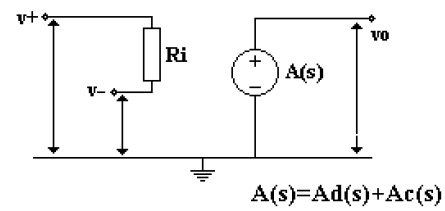
\includegraphics[width=\linewidth,height=0.32\textheight,keepaspectratio]{Imagenes/modelo_simplificado_VFA.png}
    \caption{Modelo simplificado}
  \end{subfigure}
  \begin{subfigure}{0.45\linewidth}      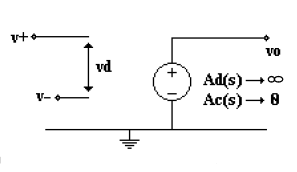
\includegraphics[width=\linewidth,height=0.32\textheight,keepaspectratio]{Imagenes/modelo_idealizado_VFA.png}
  \caption{Modelo idealizado}
  \end{subfigure}
  \caption{Modelos del VFA}
  \label{fig:modelos_VFA_2}
 \end{figure}
 
\begin{figure}[H]
    \centering
    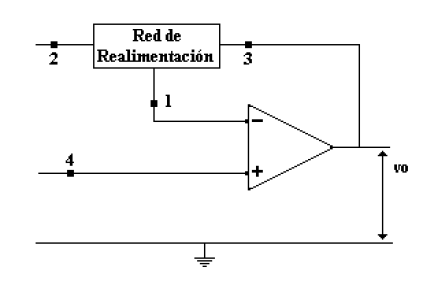
\includegraphics[width=0.45\linewidth,height=0.32\textheight,keepaspectratio]{Imagenes/esquema_realimentado.png}
    \caption{Esquema con red de realimentación}
    \label{fig:esquema_realimentado}
\end{figure}
La estructura básica de utilización de un amplificador operacional incluye una red de realimentación como se observa en la \autoref{fig:esquema_realimentado}. Dependiendo de la terminal donde se aplique la señal se tendrán distintas configuraciones. Las distintas configuraciones dependen de la red de realimentación, siendo las más comúnes: la  \textbf{no inversora} (si se excita en la terminal 4), la \textbf{inversora} (si se excita en la terminal 2) y la \textbf{diferencial}(si
se excita en las terminales 2 y 4).

\subsubsection{Configuración no inversora}
 \begin{figure}[H]
    \centering
    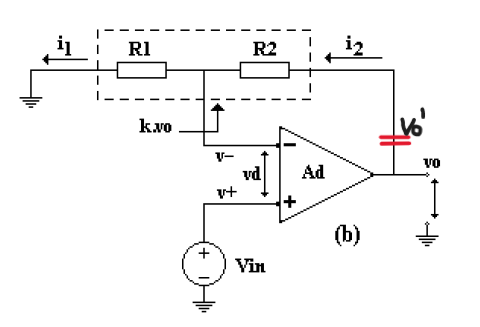
\includegraphics[width=0.5\linewidth,height=0.32\textheight,keepaspectratio]{Imagenes/config_no_inv.png}
    \caption{VFA en configuración no inversora}
    \label{fig:config_no_inv.png}
\end{figure}

Partiendo del circuito de la \autoref{fig:config_no_inv.png} se calcula la ganancia del mismo en base a la fórmula de Black, la \autoref{eq:ganancia_LC_NI}.

\begin{equation}
    A_{vf(NI)} = \frac{V_{out}}{V_{in}} = \dfrac{A_{v(NI)}}{1 - T} 
    \label{eq:ganancia_LC_NI}
\end{equation}

Donde se tiene la ganancia de lazo abierto no inversora ($A_{v(NI)}$), la ganancia de lazo ($T$) y el factor de realimentación ($K$):

\begin{align}
    A_{v(NI)} &= \left.\frac{V_o}{V_{in}}\right|_{V_o'=0} = Ad
    \label{eq:gain_LA_NI}\\
    T &= \left.\frac{V_o}{V_{o}'}\right|_{V_{in}=0} = -(\dfrac{R1}{R1+R2})\cdot Ad = - K \cdot A_{v(NI)}
    \label{eq:gain_lazo_NI}\\
    K &= (\dfrac{R1}{R1+R2})
    \label{eq:K_NI}
\end{align}

Considerando un comportamiento ideal ($ A_{d}(s) \xrightarrow[]{}{\infty}$) y reemplazando los valores de la \autoref{eq:gain_LA_NI} y la \autoref{eq:gain_lazo_NI} en la \autoref{eq:ganancia_LC_NI}  se obtiene el valor de la ganancia a lazo cerrado descripta en la \autoref{eq:ganancia_LC_NI_2}.

\begin{equation}
    A_{v(LC)} = \frac{V_{out}}{V_{in}} = \dfrac{R_2 + R_1}{R_1} = 1 + \dfrac{R2}{R1} 
    \label{eq:ganancia_LC_NI_2}
\end{equation}

\subsubsection{Errores en corriente contínua:}
 Los amplificadores operacionales tienen errores estáticos (o en corriente contínua) y dinámicos (en corriente alterna) que lo alejan de su comportamiento ideal.

 Como el objetivo del presente trabajo consiste en el comportamiento de las respuesta en frecuencia se mencionan los errores estáticos de forma anecdótica:
\begin{itemize}
    \item Off-set de tensión de entrada ($V_{OS}$).
    \item Off-set de corriente de entrada ($I_{OS}$).
    \item Error debido a la ganancia diferencial de lazo abierto finita ($A_d \neq \infty $).
    \item Error debido a la ganancia común de lazo abierto no nula ($A_c \neq 0$).
\end{itemize}
 
\subsubsection{Respuesta en Frecuencia}
Los errores dinámicos se asocian a la disminución de la ganancia a lazo abierto $A_{d(LA)}(s)$ en función de la frecuencia, debido a los polos internos del amplificador operacional.
Partiendo de un modelo básico de un amplificador con un solo polo y una ganancia diferencial definida por la \autoref{eq:gain_LA_rta_frec}

\begin{equation}
    A_d(s) = \frac{A_d(0)}{1 + \frac{s}{\omega_1}}
    \label{eq:gain_LA_rta_frec}
\end{equation}

Aplicando la fórmula de Black para el cálculo de la ganancia a lazo cerrado de este amplificador en \textbf{configuración no inversora} se obtiene la \autoref{eq:gain_LC_rta_frec}.

\begin{equation}
    A_{vf}(s) = \left[\frac{A_d(0)}{1+K.A_d(0)}\right]\cdot\left[\frac{1}{1+\dfrac{s}{\omega_1\cdot(1+K.A_d(0))}}\right] = \frac{A_{vf}(0)}{\left(1+\dfrac{s}{\omega_H}\right)}
    \label{eq:gain_LC_rta_frec}
\end{equation}


Se observa que al aplicar realimentación negativa mediante un factor $K$, el polo del sistema se desplaza hacia altas frecuencias, expandiendo el ancho de banda a lazo cerrado ($\omega_H$). Dicho ancho de banda está dado por la \autoref{eq:frecuencia_high}.

\begin{equation}
    \omega_H = \omega_1 \cdot (1- T_o) = \omega_1 \cdot (1+ K \cdot A_d(0)) \cong \omega_1 \cdot K \cdot A_d(0)) = \omega_T \cdot K
    \label{eq:frecuencia_high}
\end{equation}
Tal que el \textbf{producto de la ganancia (GBW) por el ancho de banda se mantiene constante}, como se observa en la \autoref{eq:GBW_cte}.

\begin{equation}
    GBW = A_{vf}(0) \cdot \omega_H = A_d(0) \cdot \omega_1 = \omega_T = cte
    \label{eq:GBW_cte}
\end{equation}

\begin{figure}[H]
    \centering
    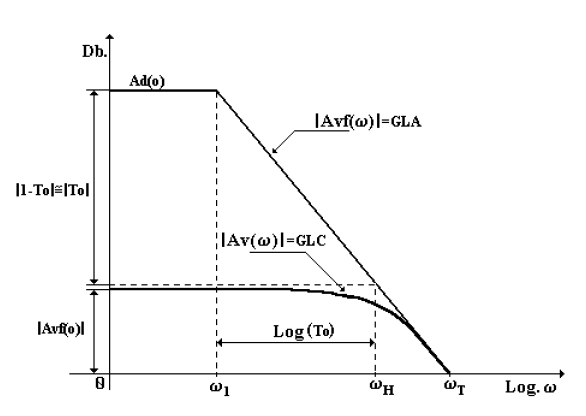
\includegraphics[width=0.5\linewidth,height=0.32\textheight,keepaspectratio]{Imagenes/ganancia_db_marco_teorico.png}
    \caption{Respuesta en frecuencia de un VFA a lazo abierto vs a lazo cerrado}
    \label{fig:ganancia_db_marco_teorico}
\end{figure}

En la \autoref{fig:ganancia_db_marco_teorico} se observa como al introducir una realimentación se aumenta el ancho de banda a costa de una reducción considerable de la ganancia del sistema. Se observa que $\omega_T$ corresponde a la frecuencia para la cual el módulo de la ganancia en decibeles es nula, es decir, ganancia unitaria (en veces).

\subsection{Amplificadores Realimentados por Corriente (CFA)}
El Amplificador Realimentado por Corriente (CFA), o amplificador de transimpedancia, posee una arquitectura interna diferente, requiriendo un menor número de etapas, lo que se traduce en velocidades de operación drásticamente superiores (mayores a $100\text{ MHz}$) y Slew-Rates que pueden superar los $1000\text{ V/}\mu\text{s}$.

\subsubsection{Características Principales}

\begin{figure}[H]
    \centering
    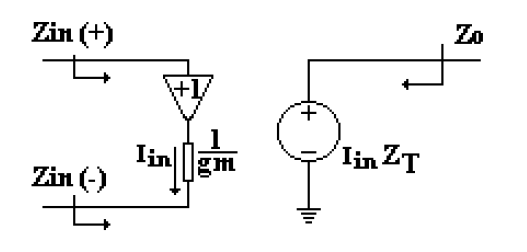
\includegraphics[width=0.5\linewidth,height=0.32\textheight,keepaspectratio]{Imagenes/modelo_CFA.png}
    \caption{Modelo compacto del CFA}
    \label{fig:modelo_CFA}
\end{figure}

A diferencia del VFA, el CFA presenta una arquitectura asimétrica en sus terminales de entrada. El terminal no inversor posee una alta impedancia (entrada a un buffer), mientras que el terminal inversor presenta una impedancia muy baja (típicamente alrededor de $20\,\Omega$, siendo la salida de dicho buffer).

En el CFA, la tensión del terminal de salida es proporcional a la corriente de error que ingresa por el terminal inversor ($I_{in}$). Por ende, el parámetro de transferencia es una transimpedancia ($Z_t$), $V_o = Z_t\,I_{in}$. En la banda de utilización puede modelarse con un único polo, pero para estudiar la estabilidad y las frecuencias altas se requiere el modelo de dos polos del apunte, \autoref{eq:trasimpedancia}:

\begin{equation}
    Z_t(s) = \frac{R_t}{\left(1 + \dfrac{s}{\omega_{t1}}\right)\left(1 + \dfrac{s}{\omega_{t2}}\right)} \qquad \omega_{t1} = \frac{1}{R_t\,C_t}
    \label{eq:trasimpedancia}
\end{equation}

Donde $R_t$ es la transresistencia (del orden del megaohm; \SI{2,37}{M\ohm} para el LM6181), $C_t$ es la transcapacitancia interna (del orden de pocos picofaradios; \SI{4,8}{pF} para el LM6181, \autoref{tab:param_cfa}), $f_{t1}=\SI{14}{kHz}$ es el polo dominante y $f_{t2}=\SI{82,3}{MHz}$ es el segundo polo, de alta frecuencia. La consigna provee $R_t$ y el apunte los polos; por eso se trabaja con $Z_t$ de dos polos y no con el modelo simple de un polo.

\subsubsection{Configuración no inversora}
\begin{figure}[H]
    \centering
    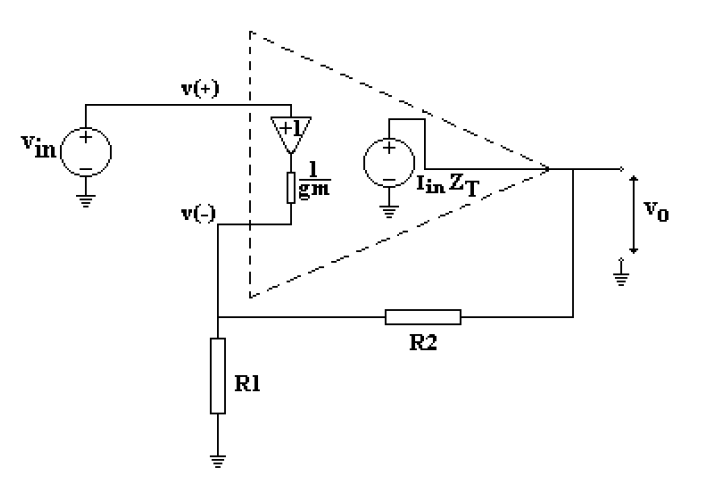
\includegraphics[width=0.5\linewidth,height=0.32\textheight,keepaspectratio]{Imagenes/CFA_NI.png}
    \caption{CFA en configuración no inversora}
    \label{fig:CFA_NI}
\end{figure}

El buffer interno entrega la tensión $V_+$ al terminal inversor a través de su resistencia de salida $r_i$ (baja, del orden de $20$ a $30\,\Omega$; el fabricante no la publica). Sea $I_{in}$ la corriente que entrega el buffer. En el nodo inversor, con $V_n = V_+ - r_i I_{in}$:
\begin{equation}
    I_{in} = \frac{V_n}{R_1} + \frac{V_n - V_o}{R_2} \qquad V_o = Z_t\,I_{in}
\end{equation}
Despejando $I_{in}$ y multiplicando por $R_2$ se obtiene
\begin{equation}
    I_{in}\left[R_2 + r_i\left(1+\tfrac{R_2}{R_1}\right) + Z_t\right] = V_+\left(1+\tfrac{R_2}{R_1}\right)
\end{equation}
Llamando $A_{vfi} = 1 + R_2/R_1$ (ganancia ideal, $Z_t\to\infty$) y $R_{eff} = R_2 + r_i\,A_{vfi}$, la ganancia a lazo cerrado queda
\begin{equation}
    A_{vf}(s) = \frac{A_{vfi}}{1 + \dfrac{R_{eff}}{Z_t(s)}} = \frac{A_{vfi}\,Z_t}{Z_t + R_{eff}}
    \label{eq:Avf_CFA_ri}
\end{equation}
que coincide con la expresión del apunte (Ec.~3.12). La ganancia de lazo es $T(s) = -Z_t(s)/R_{eff}$: depende de $Z_t$ y de $R_{eff}$, \emph{no} de la ganancia $A_{vfi}$ más que a través del término $r_i A_{vfi}$.

\subsubsection{Respuesta en Frecuencia y Estabilidad}
La principal ventaja de la arquitectura CFA reside en su respuesta dinámica. Con $Z_t$ de un polo, $Z_t \cong R_t/(1+sR_tC_t)$, y $R_t \gg R_{eff}$, la \autoref{eq:Avf_CFA_ri} resulta
\begin{equation}
    A_{vf}(s) \cong \frac{A_{vfi}}{1 + s\,C_t\,R_{eff}} \qquad \omega_H \cong \frac{1}{C_t\,R_{eff}} \cong \frac{1}{C_t\,R_2}
    \label{eq:wH_CFA}
\end{equation}
donde la última igualdad vale cuando $r_iA_{vfi} \ll R_2$. El ancho de banda queda fijado casi por completo por $R_2$ y $C_t$, y es prácticamente independiente de la ganancia: para cambiar $A_{vfi}$ se varía solo $R_1$. Esto rompe con la limitación $f_T = A_{vf}\cdot BW$ de los VFA. Cuando $A_{vfi}$ es grande, el término $r_iA_{vfi}$ no es despreciable y el ancho de banda decrece, razón por la cual el diseño usa $R_{eff}$.

Debido a que el ancho de banda es fijado por $R_{eff}$, la resistencia $R_2$ no puede elegirse arbitrariamente: se utiliza como herramienta de diseño para asegurar el margen de fase. Con el segundo polo de $Z_t$, la ganancia de lazo se cruza con 0 dB donde $|Z_t| = R_{eff}$, es decir $f_{cruce} \cong f_{t1}\,R_t/R_{eff}$, y el margen de fase es
\begin{equation}
    M_{\varphi,CFA} = 180^\circ - \left|\angle Z_t(jf_{cruce})\right| \cong 90^\circ - \arctan\frac{f_{cruce}}{f_{t2}}
    \label{eq:Mphi_CFA}
\end{equation}
Un $R_{eff}$ pequeño lleva el cruce hacia $f_{t2}$ y degrada el margen de fase; uno grande lo mejora pero reduce el ancho de banda. El fabricante recomienda $R_2 = \SI{820}{\ohm}$ para el LM6181 (el apunte indica valores cercanos a $1\,\mathrm{k}\Omega$) como compromiso entre velocidad y estabilidad.

\subsection{Estabilidad en Amplificadores}

La estabilidad de un amplificador realimentado es un aspecto relevante en el diseño, ya que determina la capacidad del sistema para operar sin oscilaciones indeseadas. El análisis de estabilidad se puede evaluar a través de la función de transferencia a lazo abierto $|A_v(jw)|$ o de la función de ganancia de lazo $|T(jw)|$, observando su comportamiento en el dominio de la frecuencia y su impacto en la respuesta transitoria.

Para ello se utiliza el método gráfico donde si se usa la función de $|A_v(jw)|$ se busca su intersección con la recta de valor $\frac{1}{K}$ o en el caso de usar la función de $|T(jw)|$ se busca su intersección con $|T(jw)|=0\ dB$. Mediante estos puntos se determinan las condiciones de estabilidad: el margen de fase $M_\phi$ y el margen de ganancia $M_G$.

\subsubsection{Margen de Fase y Margen de Ganancia}

Para cuantificar qué tan alejado se encuentra un sistema del punto crítico de inestabilidad, se definen dos métricas fundamentales sobre el diagrama de Bode de la ganancia de lazo abierto $T(j\omega)$:

\begin{itemize}
    \item \textbf{Margen de Fase ($M\phi$):} Se define como el desfasaje adicional que puede introducirse en el lazo, evaluado en la frecuencia de cruce de ganancia $\omega_{gc}$ (donde el módulo $|T(j\omega_{gc})| = 1$ o $0\text{ dB}$), antes de que el sistema alcance el límite teórico de inestabilidad ($-180^\circ$). Matemáticamente se expresa como:
    \begin{equation}
        MF = 180^\circ + \angle T(j\omega_{gc})
    \end{equation}

    \item \textbf{Margen de Ganancia (MG):} Representa el incremento adicional de ganancia que el sistema puede tolerar antes de volverse inestable. Se evalúa en la frecuencia de cruce de fase $\omega_{pc}$, donde el desfasaje de la función de lazo alcanza exactamente los $-180^\circ$. Se calcula en decibelios a través de la expresión:
    \begin{equation}
        MG = -20 \log_{10} |T(j\omega_{pc})|
    \end{equation}
\end{itemize}

\subsubsection{Medición del Margen de Fase a través de la Respuesta al Escalón}
\label{sec:escalon_mf}

Aunque el margen de fase es un concepto puramente del dominio de la frecuencia, existe una correlación analítica directa con el dominio del tiempo para sistemas dominados por una dinámica de segundo orden. Esta relación permite estimar la estabilidad observando la respuesta transitoria frente a una excitación escalón.

Cuando un sistema de segundo orden subamortiguado es excitado, la tensión de salida presenta un sobrepico antes de alcanzar su valor de estado estacionario. El sobrepico porcentual ($\mathrm{\char37}OS$) se calcula midiendo la diferencia entre la tensión pico $V_{pico}$ y la tensión final $V_{estacionario}$:
\begin{equation}
    \mathrm{\char37}OS = \frac{V_{pico} - V_{estacionario}}{V_{estacionario}} \cdot 100
    \label{eq:OS}
\end{equation}

La magnitud de este sobrepico está directamente vinculada al factor de amortiguamiento $\zeta$ del sistema equivalente mediante la siguiente relación analítica:
\begin{equation}
    \zeta = \frac{-\ln\left(\frac{\mathrm{\char37}OS}{100}\right)}{\sqrt{\pi^2 + \ln^2\left(\frac{\mathrm{\char37}OS}{100}\right)}}
    \label{eq:zeta}
\end{equation}

A su vez, el factor de amortiguamiento $\zeta$ define de manera unívoca el margen de fase del circuito cerrado. Para el análisis teórico riguroso, la relación trigonométrica exacta entre ambas variables está dada por:
\begin{equation}
    MF = \arctan\left( \frac{2\zeta}{\sqrt{\sqrt{1+4\zeta^4}-2\zeta^2}} \right)
    \label{eq:MF_exacta}
\end{equation}

De manera práctica, para valores moderados del amortiguamiento ($0{,}5 \lesssim \zeta \lesssim 0{,}6$) se admite una aproximación lineal, con un error menor a $2^\circ$:
\begin{equation}
    MF \approx 100 \cdot \zeta \quad \text{(en grados)}
    \label{eq:MF_aprox}
\end{equation}
Para máxima planicidad de módulo ($\zeta = 0{,}707$) esta aproximación sobreestima el margen de fase en unos $5^\circ$ (resulta $70{,}7^\circ$ frente a $65{,}5^\circ$ exactos), por lo que en este trabajo se utiliza la relación exacta (\autoref{eq:MF_exacta}).

En consecuencia, el registro y medición de la respuesta al escalón (ya sea mediante simulación o instrumentación física) constituye un método robusto para deducir el amortiguamiento $\zeta$ y, consecuentemente, certificar el margen de fase y la estabilidad del amplificador compuesto.

\subsubsection{Respuesta de máxima planicidad de módulo (MPM)}
\label{sec:mpm}

Un sistema realimentado cuya ganancia de lazo $T(s)$ tiene dos polos presenta también una ganancia a lazo cerrado con dos polos, cuyo carácter (reales o complejos conjugados) depende de la cantidad de realimentación introducida. Si el numerador no tiene ceros, la respuesta normalizada respecto de su valor en continua y de la frecuencia de los polos $\omega_p$ (módulo de los polos, o frecuencia natural), con $S = s/\omega_p$ y $\Omega = \omega/\omega_p$, es:
\begin{equation}
    a_f(S) = \frac{A_{vf}(s)}{A_{vf}(0)} = \frac{1}{1 + \dfrac{S}{Q_p} + S^2}
    \label{eq:2orden}
\end{equation}
donde $Q_p$ es el factor de calidad de los polos ($\zeta = 1/2Q_p$). Su módulo al cuadrado resulta:
\begin{equation}
    |a_f(j\Omega)|^2 = \frac{1}{(1-\Omega^2)^2 + \dfrac{\Omega^2}{Q_p^2}} = \frac{1}{1 + \left(\dfrac{1}{Q_p^2}-2\right)\Omega^2 + \Omega^4}
    \label{eq:mod2orden}
\end{equation}

\paragraph{Condición de máxima planicidad.} Para que el módulo sea constante con la frecuencia, los coeficientes de las potencias homólogas del numerador y del denominador de $|a_f|^2$ deben ser iguales. Como el numerador es la unidad (sus coeficientes son nulos), la única condición que puede satisfacerse es anular el coeficiente de $\Omega^2$:
\begin{equation}
    \frac{1}{Q_p^2} - 2 = 0 \quad \Rightarrow \quad Q_p = \frac{1}{\sqrt{2}} = 0{,}707
    \label{eq:Q_MPM}
\end{equation}
En ese caso el módulo queda $|a_f(j\Omega)|^2 = 1/(1+\Omega^4)$ (respuesta de Butterworth), sin sobrepico. La frecuencia de corte a $-3\text{ dB}$ se obtiene de $1/(1+\Omega_H^4) = 1/2$, es decir $\Omega_H = 1$:
\begin{equation}
    \omega_H = \omega_p
    \label{eq:wH_wp}
\end{equation}
Esto es, en MPM el ancho de banda real coincide con la frecuencia natural de los polos. Para un $Q_p$ cualquiera, la frecuencia de corte surge de igualar a $2$ el denominador de \autoref{eq:mod2orden}:
\begin{equation}
    \Omega_H^2 = a + \sqrt{a^2+1}, \quad a = 1 - \frac{1}{2Q_p^2} \qquad\Rightarrow\qquad f_H = f_p\sqrt{a + \sqrt{a^2+1}}
    \label{eq:polos_BW}
\end{equation}
(para $Q_p = 1/\sqrt{3}$, máxima planicidad de retardo, resulta $f_H = 0{,}786\,f_p$). Los polos de lazo cerrado son $s_{1,2} = -\dfrac{\omega_p}{2Q_p} \pm j\,\omega_p\sqrt{1 - \dfrac{1}{4Q_p^2}}$, que para MPM forman un ángulo de $45^\circ$ con el eje real: $s_{1,2} = -\dfrac{\omega_p}{\sqrt{2}}(1 \mp j)$.

\paragraph{Ganancia de lazo asociada.} Con la fórmula de Black modificada $A_{vf}(s) = A_{vfi}/(1 - 1/T(s))$ y la \autoref{eq:2orden}, resulta $1 - 1/T = 1 + S/Q_p + S^2$, y por lo tanto la ganancia de lazo normalizada es:
\begin{equation}
    T(S) = -\frac{1}{\dfrac{S}{Q_p} + S^2} = -\frac{1}{S\left(S + \dfrac{1}{Q_p}\right)}
    \label{eq:T_norm}
\end{equation}
Es decir, un polo en el origen (el polo dominante $\omega_{p1}$, despreciable frente a $\omega_p$) y otro en $\omega_p/Q_p = \sqrt{2}\,\omega_p$.

\paragraph{Punto crítico y margen de fase.} La frecuencia crítica $\Omega_G$ se obtiene imponiendo $|T(j\Omega_G)| = 1$ en la \autoref{eq:T_norm}:
\begin{equation}
    \Omega_G^4 + \frac{1}{Q_p^2}\,\Omega_G^2 - 1 = 0 \;\;\xrightarrow{\;Q_p = 1/\sqrt{2}\;}\;\; \Omega_G = 0{,}644 \quad\Rightarrow\quad \omega_{Gc} = 0{,}644\,\omega_p
    \label{eq:omegaG}
\end{equation}
donde $\omega_{Gc}$ es la frecuencia de cruce de la ganancia de lazo \emph{compensada} (en el apunte de la cátedra se la denomina $\omega_G$; aquí se la distingue del ancho de banda potencial, \autoref{sec:bw}). El margen de fase resulta:
\begin{equation}
    M_\varphi = 180^\circ + \angle T(\Omega_G) = 180^\circ - 90^\circ - \arctan\left(\Omega_G\,Q_p\right) = 65{,}5^\circ
    \label{eq:Mphi_MPM}
\end{equation}
que es el valor especificado en la consigna ($M_\varphi \approx \ang{65}$ o, equivalentemente, $Q_p = 0{,}707$) y coincide con el obtenido de la \autoref{eq:MF_exacta} para $\zeta = 1/(2Q_p) = 0{,}707$.

\paragraph{Relaciones de diseño.} En un amplificador compuesto la ganancia de lazo puede aproximarse con dos polos, $\omega_{p1} \ll \omega_{p2}$:
\begin{equation}
    T(s) = - \frac{T_0}{\left(1 + \dfrac{s}{\omega_{p1}}\right)\left(1 + \dfrac{s}{\omega_{p2}}\right)} \qquad T_0 = |T(0)|
    \label{eq:lazo2polos}
\end{equation}
Introduciendo esta expresión en la fórmula de Black modificada:
\begin{equation}
    A_{vf}(s) = \frac{A_{vfi}}{1 + \dfrac{1}{T_0}\left(1+\dfrac{s}{\omega_{p1}}\right)\left(1+\dfrac{s}{\omega_{p2}}\right)} \cong \frac{A_{vfi}}{1 + \dfrac{s}{T_0\,\omega_{p1}} + \dfrac{s^2}{T_0\,\omega_{p1}\,\omega_{p2}}}
    \label{eq:Avf_dospolos}
\end{equation}
donde se utilizaron $T_0 \gg 1$ y $D_p = \omega_{p2}/\omega_{p1} \gg 1$ (separación de polos). Comparando con la \autoref{eq:2orden}, y definiendo $A = T_0/D_p$:
\begin{equation}
    \omega_p^2 = T_0\,\omega_{p1}\,\omega_{p2} \;\Rightarrow\; \omega_p = \omega_{p2}\sqrt{A} \qquad\qquad \frac{1}{Q_p} = \frac{\omega_p}{T_0\,\omega_{p1}} = \frac{1}{\sqrt{A}} \;\Rightarrow\; Q_p^2 = A = \frac{T_0}{D_p}
    \label{eq:wp_A}
\end{equation}
Para MPM ($Q_p^2 = 1/2$) la separación de polos debe ser, entonces:
\begin{equation}
    D_p = 2\,T_0 \qquad\Rightarrow\qquad \omega_p = \frac{\omega_{p2}}{\sqrt{2}}
    \label{eq:Dp_MPM}
\end{equation}
Por último, el margen de fase de un lazo de dos polos cualquiera se calcula en su frecuencia crítica $f_{Gc}$, solución de $|T(j2\pi f_{Gc})| = 1$:
\begin{equation}
    M_\varphi = 180^\circ - \arctan\frac{f_{Gc}}{f_{p1}} - \arctan\frac{f_{Gc}}{f_{p2}}
    \label{eq:Mphi_2polos}
\end{equation}
Con $\omega_{p1}\to 0$ y $\omega_{p2} = \sqrt{2}\,\omega_p$ esta expresión coincide con la \autoref{eq:Mphi_MPM}.

\subsection{Amplificadores compuestos}

Se entiende por estructuras compuestas a aquellas configuraciones que incorporan más de un amplificador participando dentro del lazo de realimentación principal. El objetivo de esta topología es lograr un comportamiento global que conserve y potencie las características relevantes de cada dispositivo individual, minimizando al mismo tiempo sus debilidades intrínsecas. Una de las conexiones más utilizadas consiste en disponer dos amplificadores operacionales en cascada dentro del lazo, como se observa en la \autoref{fig:MT_AO_compuesto}.

\begin{figure}[H]
    \centering
    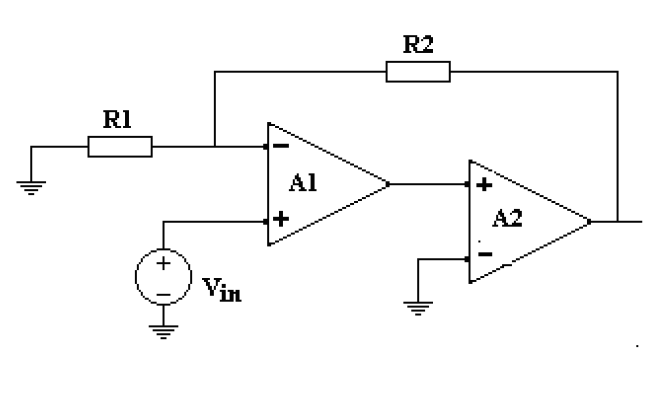
\includegraphics[width=0.5\linewidth,height=0.32\textheight,keepaspectratio]{Imagenes/MT_AO_compuesto.png}
    \caption{Amplificador compuesto}
    \label{fig:MT_AO_compuesto}
\end{figure}

Si bien la topología compuesta mejora considerablemente las características del circuito al usarse con amplificadores con características distintas se plantea el caso teórico de utilizar dos amplificadores idénticos, con el mismo modelo y topología.

\begin{figure}[H]
    \centering
    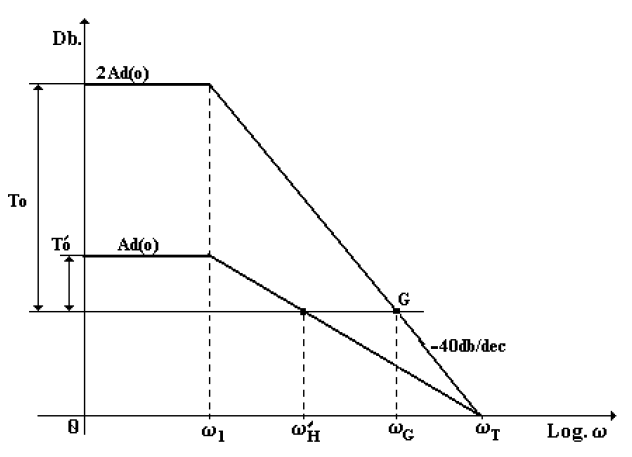
\includegraphics[width=0.5\linewidth,height=0.32\textheight,keepaspectratio]{Imagenes/MT_AO_compuesto_rta_frec.png}
    \caption{Respuesta en frecuencia del amplificador compuesto}
    \label{fig:MT_AO_compuesto_rta_frec}
\end{figure}

Como se observa en la \autoref{fig:MT_AO_compuesto_rta_frec}, la ganancia de lazo abierto del sistema compuesto se incrementa significativamente ($2 \cdot A_{d0}$) y también se introduce un polo doble $\omega_1$. Al compararse con la respuesta en frecuencia de una configuración de un solo amplificador se observa que para una misma ganancia $\frac{1}{K_c}$ el circuito con los amplificadores compuestos obtienen un ancho de banda mucho mayor ($\omega_G > \omega_H$).

Este polo doble puede inducir un desfase excesivo, reduciendo el margen de fase y comprometiendo la estabilidad del sistema. Por lo tanto, es crucial implementar técnicas de compensación para garantizar un comportamiento estable y predecible del amplificador compuesto.


\subsubsection{Ancho de banda potencial y ancho de banda real}
\label{sec:bw}

En el análisis de los amplificadores compuestos se emplean varias frecuencias que conviene distinguir, porque se obtienen de curvas distintas y con criterios distintos:

\begin{itemize}
    \item \textbf{Ancho de banda potencial ($f_G$):} es la frecuencia del punto crítico $G$ de la estructura, donde la ganancia de lazo cruza $0\text{ dB}$ (o, equivalentemente, donde la ganancia de lazo abierto $|A_v|$ se iguala a $1/K$). Representa el máximo ancho de banda que admite la estructura para la ganancia $A_{vf}$ pedida. Se calcula a partir de la ganancia de lazo y no se mide directamente sobre $A_{vf}(s)$.
    \item \textbf{Ancho de banda real ($f_H$):} es la frecuencia a la que el módulo de la ganancia a lazo cerrado cae $3\text{ dB}$ respecto de su valor en continua, $|A_{vf}(j\omega_H)| = A_{vf}(0)/\sqrt{2}$. Se puede calcular a partir de la función de transferencia a lazo cerrado (\autoref{eq:polos_BW}) y se puede medir sobre el circuito simulado o armado.
    \item \textbf{Frecuencia de los polos de lazo cerrado ($f_p$):} es el módulo de los polos de la función de transferencia a lazo cerrado (frecuencia natural, \autoref{eq:wp_A}). Para $Q_p = 1/\sqrt{2}$ coincide con el ancho de banda real (\autoref{eq:wH_wp}).
\end{itemize}

Cuando la respuesta es de máxima planicidad de módulo ($Q_p = 1/\sqrt{2}$) las tres magnitudes anteriores se relacionan de forma simple: el ancho de banda real coincide con la frecuencia de los polos y, para el compuesto compensado por desplazamiento (\autoref{eq:wH_MPM}), también con el ancho de banda potencial:
\begin{equation}
    f_H = f_p = f_G \qquad (Q_p = 1/\sqrt{2})
    \label{eq:fH_fp_MPM}
\end{equation}
Para cualquier otro $Q_p$ la igualdad no se cumple: con $Q_p<1/\sqrt{2}$ la respuesta es más amortiguada y $f_H$ difiere de $f_p$ (\autoref{eq:wH_wp}).

\paragraph{Amplificador simple.} De la \autoref{eq:frecuencia_high}, el ancho de banda del amplificador con una sola etapa es
\begin{equation}
    f_H' \cong K\, f_T = \frac{f_T}{A_{vf}}
    \label{eq:bw_simple}
\end{equation}

\paragraph{Amplificador compuesto sin compensar.} Este resultado es el del apunte (Cap.~VII, Fig.~7.18). Para $\omega \gg \omega_1$ cada amplificador se comporta como $A_d(j\omega) \cong \omega_T/(j\omega)$, de modo que con dos amplificadores idénticos $|A_v(j\omega)| \cong (\omega_T/\omega)^2$. El punto crítico se obtiene de la condición $|A_v(j\omega_G)| = 1/K = A_{vf}$:
\begin{equation}
    \omega_G = \frac{\omega_T}{\sqrt{A_{vf}}} \qquad\Rightarrow\qquad \frac{f_G}{f_H'} = \sqrt{A_{vf}}
    \label{eq:wG}
\end{equation}
Es decir, el ancho de banda potencial del compuesto es función inversa de la raíz cuadrada de la ganancia a lazo cerrado, y mejora en un factor $\sqrt{A_{vf}}$ al del amplificador simple. Sin embargo, el cruce ocurre con una pendiente de $-40\text{ dB/dec}$ (polo doble), por lo que el margen de fase es prácticamente nulo y es necesario compensar.

\paragraph{Amplificador compuesto compensado por desplazamiento.} Al compensar, la ganancia de lazo cruza $0\text{ dB}$ con pendiente de $-20\text{ dB/dec}$. En la zona $\omega_1 \ll \omega \ll \omega_{px}$ resulta $|T| \cong T_0\,\omega_1/\omega = K\,A_{vf2}\,\omega_T/\omega$, de donde
\begin{equation}
    \omega_{Gc} \cong K\, A_{vf2}\,\omega_T
    \label{eq:wGc}
\end{equation}
Esta frecuencia de cruce de la ganancia de lazo \textbf{compensada} ($f_{Gc}$) es la que se mide en el simulador sobre el circuito de ganancia de lazo y con la que se calcula el margen de fase. Es menor que el potencial, porque la compensación reduce la ganancia de lazo. En cambio, el ancho de banda real de la respuesta a lazo cerrado con máxima planicidad vale (\autoref{sec:mpm}) $f_H = f_p = f_{px}/\sqrt{2}$, que con $A_{vf2} = Q_p\sqrt{A_{vf}}$ (\autoref{eq:Avf2_MPM}) resulta
\begin{equation}
    f_H = \frac{f_{px}}{\sqrt{2}} = \frac{f_T}{\sqrt{2}\,A_{vf2}} = \frac{f_T}{\sqrt{A_{vf}}} = f_G
    \label{eq:wH_MPM}
\end{equation}
En consecuencia, la compensación por desplazamiento \textbf{recupera como ancho de banda real el ancho de banda potencial} del compuesto sin compensar, a costa de perder ganancia de lazo (precisión estática). Además, para MPM se verifica $f_H = \sqrt{2}\,f_{Gc}$.

\begin{table}[H]
\centering
\caption{Resumen de las frecuencias características del amplificador compuesto.}
\label{tab:resumen_bw}
\small
\begin{tabularx}{\textwidth}{>{\raggedright\arraybackslash}p{3.6cm} >{\raggedright\arraybackslash}X >{\raggedright\arraybackslash}X}
\toprule
\textbf{Magnitud} & \textbf{Definición} & \textbf{Cómo se obtiene} \\
\midrule
Ancho de banda potencial $f_G$ & Punto crítico $G$ de la estructura sin compensar ($|T| = 1$ con $-40\text{ dB/dec}$) & Cálculo: $f_T/\sqrt{A_{vf}}$ \\
Cruce de la ganancia de lazo compensada $f_{Gc}$ & $|T(jf_{Gc})| = 1$ con la compensación implementada & Cálculo: $K\,A_{vf2}\,f_T$. Simulación del circuito de ganancia de lazo \\
Polos de lazo cerrado $f_p$ & Módulo de las raíces de $1 - T(s) = 0$ & Cálculo con \autoref{eq:wp_A} \\
Ancho de banda real $f_H$ & $|A_{vf}(jf_H)| = A_{vf}(0)/\sqrt{2}$ ($-3\text{ dB}$) & Cálculo: \autoref{eq:wH_wp} y \autoref{eq:polos_BW}. Simulación AC o medición \\
\bottomrule
\end{tabularx}
\end{table}

\subsubsection{Compensación por desplazamiento (Separación de polos)}

\begin{figure}[H]
    \centering
    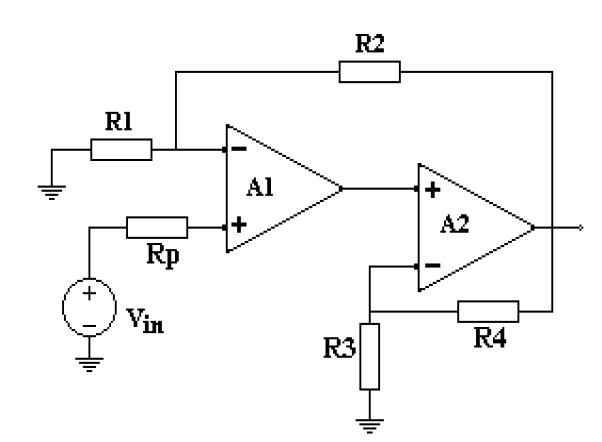
\includegraphics[width=0.5\linewidth,height=0.32\textheight,keepaspectratio]{Imagenes/MT_AO_desplazamiento.png}
    \caption{Esquemático de compensación por desplazamiento de polos}
    \label{fig:MT_AO_desplazamiento}
\end{figure}

Una solución para mitigar la inestabilidad causada por la presencia de un polo doble en la configuración compuesta consiste en separar dichos polos en el dominio de la frecuencia. Esto se logra incrementando la frecuencia de corte (y por ende, el ancho de banda) del segundo amplificador de la cascada.

\begin{figure}[H]
    \centering
    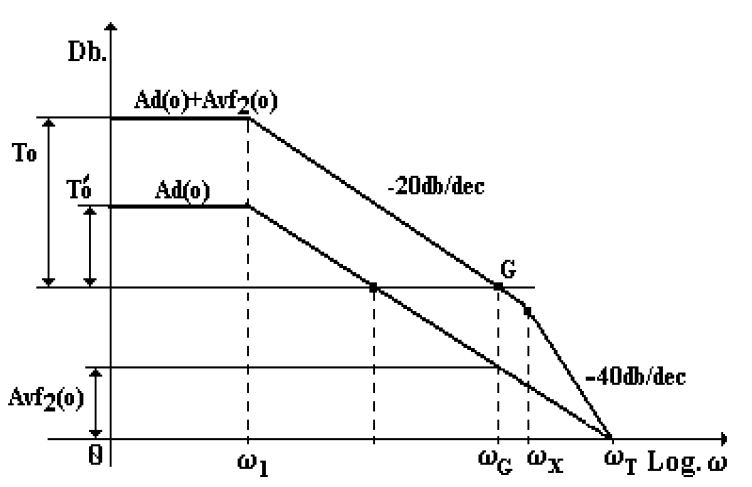
\includegraphics[width=0.5\linewidth,height=0.32\textheight,keepaspectratio]{Imagenes/MT_rta_frec_desplazamiento.png}
    \caption{Respuesta en frecuencia de la compensación por desplazamiento}
    \label{fig:MT_AO_desplazamiento_rta_frec}
\end{figure}

Para lograr este desplazamiento, se reduce la ganancia del segundo amplificador mediante un lazo de realimentación negativa interno o local, como se muestra en la \autoref{fig:MT_AO_desplazamiento}. Al disminuir su ganancia local a un valor $A_{vf2}$, su frecuencia de polo se desplaza hacia altas frecuencias ($\omega_{px}$), permitiendo que la ganancia de lazo global del sistema compuesto ($T$) cruce el eje de 0 dB con una pendiente estable de $-20$ dB/dec antes de que el segundo polo actúe, tal y como se observa en la \autoref{fig:MT_AO_desplazamiento_rta_frec}.


La separación requerida entre el primer polo dominante ($\omega_1$) y el polo desplazado ($\omega_{px}$) dependerá del tipo de respuesta deseada (por ejemplo, Máxima Planicidad de Módulo o MPM). La frecuencia del nuevo polo de compensación del segundo amplificador se determina como:
\begin{equation}
\omega_{px} = \frac{\omega_T}{A_{vf2}(0)}
\label{eq:wpx}
\end{equation}
Donde $\omega_T$ es la frecuencia de transición del amplificador. Si bien esta técnica recupera el ancho de banda potencial estableciendo un margen de fase seguro, se realiza a expensas de sacrificar una fracción de la ganancia de lazo total (precisión estática), ya que se reduce la ganancia de la segunda etapa.

\paragraph{Origen de $\omega_{px}$.} Con el lazo local de factor $K_2 = 1/A_{vf2}$ y un amplificador de un polo dominante, $A_2(s) = A_{d0}/(1+s/\omega_1)$, la ganancia de la segunda etapa realimentada es
\begin{equation}
    A_{2f}(s) = \frac{A_2}{1+K_2 A_2} = \frac{A_{d0}}{1 + \dfrac{A_{d0}}{A_{vf2}} + \dfrac{s}{\omega_1}} \cong \frac{A_{vf2}}{1 + \dfrac{s}{\omega_{px}}} \qquad \omega_{px} = \omega_1\left(1 + \frac{A_{d0}}{A_{vf2}}\right) \cong \frac{\omega_T}{A_{vf2}}
    \label{eq:A2f}
\end{equation}
es decir que el producto ganancia-ancho de banda se mantiene constante y el polo se desplaza hacia altas frecuencias al reducir la ganancia.

\paragraph{Condición de diseño para MPM.} La ganancia de lazo del compuesto queda con dos polos, $\omega_1$ y $\omega_{px}$ (\autoref{eq:lazo2polos} con $\omega_{p1} = \omega_1$ y $\omega_{p2} = \omega_{px}$), con
\begin{equation}
    T_0 = K\,A_{d0}\,A_{vf2} \qquad D_p = \frac{\omega_{px}}{\omega_1} = \frac{A_{d0}}{A_{vf2}}
\end{equation}
Reemplazando en la \autoref{eq:wp_A} se tiene $Q_p^2 = T_0/D_p = K\,A_{vf2}^2$, y al imponer $Q_p = 1/\sqrt{2}$ (equivalentemente $D_p = 2T_0$, \autoref{eq:Dp_MPM}) resulta la ganancia que debe tener la segunda etapa:
\begin{equation}
    A_{vf2} = \frac{Q_p}{\sqrt{K}} = Q_p\sqrt{A_{vf}}
    \label{eq:Avf2_MPM}
\end{equation}
\paragraph{Verificación sin aproximar.} Sin suponer $T_0 \gg 1$ ni $D_p \gg 1$, los polos de $1 - T(s) = 0$ cumplen $s^2 + (\omega_1 + \omega_{px})\,s + \omega_1\omega_{px}(1+T_0) = 0$, de donde $\omega_p^2 = \omega_1\omega_{px}(1+T_0)$ y $Q_p = \omega_p/(\omega_1+\omega_{px})$. Para el LM324, $Q_p^2$ exacto difiere de $1/2$ en un orden de $10^{-5}$, por lo que las aproximaciones de la \autoref{eq:wp_A} son válidas. Este cálculo exacto es el que realiza el cuaderno.


\subsubsection{Amplificadores compuestos de distinta topología (VFA + CFA)}
\label{sec:compuesto_distinto}

El apunte desarrolla el amplificador compuesto con dos amplificadores idénticos; no trata el caso de un VFA seguido de un CFA. Este caso es el que utiliza la técnica de ``composite amplifier'' de la literatura de aplicación (Loquinario, \emph{Analog Dialogue} 53-03, 2019): un VFA de precisión y baja tensión de offset, pero lento, se combina con un amplificador rápido dentro del mismo lazo, de modo que la exactitud en continua la fija el primero y el ancho de banda el segundo. El tratamiento que sigue es una extensión directa de las relaciones del apunte.

Sea el VFA (A01) con ganancia $A_1(s)$ y el CFA (A02) con su realimentación local. Se llama $A_{vfi2}$ a la ganancia ideal del CFA realimentado (la $A_{vfi}$ de la \autoref{eq:Avf_CFA_ri}, renombrada para distinguirla de la ganancia global) y $A_{2f}(s)$ a su respuesta en frecuencia. Con $K = 1/A_{vf}$ el factor de realimentación global, resulta
\begin{equation}
    A_1(s) = \frac{A_{d0}}{\left(1+\dfrac{s}{\omega_1}\right)\left(1+\dfrac{s}{\omega_2}\right)}
\end{equation}
y la ganancia de lazo global
\begin{equation}
    T(s) = -K\,A_1(s)\,A_{2f}(s)
\end{equation}
Como el polo de $A_{2f}$ es mucho más alto que la frecuencia crítica, en la zona de interés $A_{2f}\cong A_{vfi2}$ y $T$ queda con los dos polos del VFA:
\begin{equation}
    T(s) \cong \frac{T_0}{\left(1+\dfrac{s}{\omega_1}\right)\left(1+\dfrac{s}{\omega_2}\right)} \qquad T_0 = K\,A_{d0}\,A_{vfi2}
\end{equation}
Para $\omega \gg \omega_1$ el VFA se comporta como $\omega_T/s$, y la ganancia de lazo se reduce a $T \cong K\,A_{vfi2}\,\omega_T/s$. Su cruce asintótico ($|T|=1$) define el ancho de banda potencial
\begin{equation}
    \omega_g = K\,A_{vfi2}\,\omega_T \qquad\Rightarrow\qquad A_{vfi2} = \frac{\omega_g}{K\,\omega_T}
    \label{eq:wg_VFACFA}
\end{equation}
A diferencia del compuesto de amplificadores idénticos (donde $f_G = f_T/\sqrt{A_{vf}}$), aquí el ancho de banda lo fija la ganancia del CFA, $A_{vfi2}$. Aplicando la \autoref{eq:wp_A} con $D_p = \omega_2/\omega_1$ resulta
\begin{equation}
    Q_p^2 \cong \frac{T_0}{D_p} = \frac{K\,A_{d0}\,A_{vfi2}\,\omega_1}{\omega_2} = \frac{\omega_g}{\omega_2}
    \label{eq:Qp_VFACFA}
\end{equation}
Para MPM se exige $Q_p^2 = 1/2$, lo que limita el cruce a $\omega_g \le \omega_2/2$ y, por lo tanto, la ganancia del CFA queda acotada:
\begin{equation}
    A_{vfi2} \le A_{vfi2,max} = \frac{\omega_2}{2\,K\,\omega_T}
    \label{eq:Avfi2_max}
\end{equation}
Elegir $A_{vfi2} = A_{vfi2,max}$ da MPM en el modelo de dos polos, pero deja poco margen para los polos del CFA, que agregan atraso de fase. Por eso conviene tomar un $A_{vfi2}$ algo menor, que da $Q_p<1/\sqrt2$ (respuesta más amortiguada, sin pico) y un margen de fase mayor.

Para que la aproximación $A_{2f}\cong A_{vfi2}$ sea válida, el polo del CFA realimentado debe quedar una década por encima de $f_g$. Con $R_{eff}$ definida en la \autoref{eq:Avf_CFA_ri}:
\begin{equation}
    R_{eff} = R_2 + r_i\,A_{vfi2} \qquad f_{cfa} \cong \frac{1}{2\pi\,C_t\,R_{eff}} \ge 10\,f_g
\end{equation}
El modelo completo (cuatro polos) incluye $A_{2f}(s)$ de la \autoref{eq:Avf_CFA_ri}.

\subsubsection{Compensación cero-polo (Adelanto)}
\label{sec:adelanto}
Para aplicaciones de alta ganancia donde se requiere mantener la máxima precisión posible en continua y a su vez estabilizar el sistema frente a polos parásitos o múltiples (como en los amplificadores compuestos), la compensación por adelanto de fase, también conocida como compensación cero-polo, resulta sumamente efectiva.

Esta técnica introduce un cero ($f_{zx}$) cercano al segundo polo problemático del sistema original, de modo que corrige el atraso de fase que éste provoca antes de llegar a la frecuencia del punto crítico. Se implementa con una red resistiva-capacitiva, cuya forma básica es un divisor resistivo $R_x$--$R_y$ con un capacitor $C_x$ en paralelo con $R_x$ (\autoref{fig:red_RC_adelanto}):
\begin{equation}
    \begin{gathered}
    A_c(s) = \frac{R_y}{R_x+R_y}\cdot\frac{1+sC_xR_x}{1+sC_x\,(R_x\parallel R_y)} \\
    \omega_{zx} = \frac{1}{C_xR_x} \qquad \omega_{px} = \frac{1}{C_x\,(R_x\parallel R_y)} \qquad \frac{\omega_{px}}{\omega_{zx}} = 1+\frac{R_x}{R_y}
    \end{gathered}
    \label{eq:red_RC}
\end{equation}
La red atenúa en continua ($A_c(0) = R_y/(R_x+R_y)<1$) y a alta frecuencia recupera la ganancia unitaria; por eso el cero se ubica antes que el polo.

\begin{figure}[H]
    \centering
    \begin{tikzpicture}[x=1cm,y=1cm,line cap=round]
        \draw (0,1.2) node[left]{$v_i$} -- (0.5,1.2);
        \draw (0.5,1.2) -- (0.5,1.8) -- (1.0,1.8); \draw (2.2,1.8) -- (2.7,1.8) -- (2.7,1.2);
        \draw (1.0,1.65) rectangle (2.2,1.95); \node at (1.6,2.25){$R_x$};
        \draw (0.5,1.2) -- (0.5,0.6) -- (1.0,0.6); \draw (1.0,0.45) -- (1.0,0.75); \draw (1.25,0.45) -- (1.25,0.75); \draw (1.25,0.6) -- (2.7,0.6) -- (2.7,1.2);
        \node at (1.1,0.15){$C_x$};
        \draw (2.7,1.2) -- (3.4,1.2) node[right]{$v_o$};
        \draw (3.0,1.2) -- (3.0,0.9); \draw (2.85,0.9) rectangle (3.15,0.3); \node at (3.5,0.6){$R_y$};
        \draw (3.0,0.3) -- (3.0,0.0); \draw (2.8,0.0) -- (3.2,0.0);
    \end{tikzpicture}
    \caption{Red cero-polo: $C_x$ en paralelo con $R_x$ y $R_y$ a tierra}
    \label{fig:red_RC_adelanto}
\end{figure}

Según el lugar del lazo donde se coloca la red, el efecto es diferente (apunte, Cap. VI):
\begin{itemize}
    \item \textbf{Red en la entrada del amplificador compuesto o dentro de la red de realimentación} (por ejemplo, $C_x$ en paralelo con la resistencia de realimentación global): el cero aparece en el numerador de la ganancia de lazo,
    \begin{equation}
        T(s) \cong - \frac{T_0 \left(1 + \frac{s}{\omega_{zx}}\right)}{\left(1 + \frac{s}{\omega_{p1}}\right) \left(1 + \frac{s}{\omega_{p2}}\right)}
    \end{equation}
    y, definiendo $D_z = \omega_{zx}/\omega_{p2}$, la relación $1/Q_p = 1/\sqrt{A} + \sqrt{A}/D_z$ con $A = T_0/D_p$ (apunte, Ec.~6.40a) permite ubicar el cero para MPM. Para $D_p \gg 1$ resulta
    \begin{equation}
        f_{zx} \cong f_{p2}\,Q_p\sqrt{\frac{T_0}{D_p}}
    \end{equation}
    \item \textbf{Red a la salida del amplificador básico} (entre la salida del VFA y la entrada del siguiente amplificador): el cero queda en el numerador de la ganancia a lazo cerrado y se elige $D_x = \omega_{zx}/\omega_{p2} \cong 1$ (apunte, Ec.~6.50 y 6.51), de modo que el cero \emph{cancela} el segundo polo del amplificador. La ganancia de lazo queda con dos polos, $\omega_{p1}$ y el polo de la red $\omega_{px}$, y es éste (más alto que $\omega_{p2}$) el que define el nuevo segundo polo.
\end{itemize}

La ventaja fundamental de la compensación por adelanto es que recupera o extiende el ancho de banda potencial sin degradar la ganancia de lazo en continua $T_0$, siempre que la atenuación $A_c(0)$ de la red se compense con ganancia adicional en alguna etapa (en el compuesto VFA + CFA, retocando $A_{vfi2}$). En la práctica la cancelación es aproximada, pues depende de las tolerancias de $R_x$ y $C_x$ y de la impedancia de salida del amplificador que alimenta a la red. En las expresiones, $Q_p$ y $D_p$ son el factor de calidad y la separación de polos definidos en la \autoref{sec:mpm}.

\newpage
\section{Desarrollo: Caso 1, configuración VFA-VFA}
\label{sec:desarrollo_c1}

\subsection{Diseño}
\label{sec:diseno_c1}

Partiendo de las características del amplificador LM324 (\autoref{tab:param_vfa}) se dimensionaron las resistencias $R_i$, $R_f$, $R_1$ y $R_2$. El segundo amplificador ($A_{02}$) está dentro del lazo global, por lo que la ganancia a lazo cerrado queda fijada por la red $R_i$--$R_f$ (\autoref{eq:ganancia_LC_NI_2}). La máxima planicidad de módulo ($Q_p = 0{,}707$) se logra compensando por desplazamiento de polos con la red local $R_1$--$R_2$ de $A_{02}$, para lo cual la ganancia de la segunda etapa debe ser $A_{vf2} = Q_p\sqrt{A_{vf}}$ (\autoref{eq:Avf2_MPM}).

Los cálculos se automatizaron en un cuaderno de Jupyter (Caso 1). En la \autoref{tab:parametros_vfa_vfa} se reúnen las expresiones utilizadas, su evaluación numérica y el valor resultante de cada parámetro de diseño, junto con la verificación de la condición de MPM ($D_p = 2T_0$, \autoref{eq:Dp_MPM}).

\begin{table}[H]
\centering
\caption{Diseño VFA-VFA con $Q_p = 0{,}707$: expresiones, cálculo y valores.}
\label{tab:parametros_vfa_vfa}
\footnotesize
\setlength{\tabcolsep}{4pt}
\begin{tabular}{>{\raggedright\arraybackslash}p{0.31\textwidth} >{\centering\arraybackslash}p{0.2\textwidth} >{\centering\arraybackslash}p{0.27\textwidth} >{\centering\arraybackslash}p{0.13\textwidth}}
\toprule
\textbf{Parámetro} & \textbf{Expresión} & \textbf{Cálculo} & \textbf{Valor} \\
\midrule
Ganancia a lazo cerrado global $A_{vf}$ & dato & \SI{20}{dB} $\rightarrow 10^{20/20}$ & \SI{10}{V/V} \\
Factor de realimentación $K$ & $1/A_{vf}$ & $1/10$ & \num{0,1} \\
Resistencia de entrada global $R_i$ & elegida & --- & \SI{10}{k\ohm} \\
Resistencia de realimentación global $R_f$ & $R_i\,(A_{vf}-1)$ & $10\text{ k}\Omega \cdot 9$ & \SI{90}{k\ohm} \\
Ganancia del segundo amplificador $A_{vf2}$ & $Q_p\sqrt{A_{vf}}$ & $0{,}707\cdot\sqrt{10}$ & \SI{2,236}{V/V} \\
Resistencia de entrada local $R_1$ & elegida & --- & \SI{10}{k\ohm} \\
Resistencia de realimentación local $R_2$ & $R_1\,(A_{vf2}-1)$ & $10\text{ k}\Omega\cdot 1{,}236$ & \SI{12,361}{k\ohm} \\
Frecuencia del polo desplazado $f_{px}$ & $f_T/A_{vf2}$ & $1\text{ MHz}/2{,}236$ & \SI{447,2}{kHz} \\
Ganancia de lazo en continua $T_0$ & $K\,A_{d0}\,A_{vf2}$ & $0{,}1\cdot 10^5 \cdot 2{,}236$ & \num{22361} (\SI{87,0}{dB}) \\
Separación de polos $D_p$ & $A_{d0}/A_{vf2}$ & $10^5/2{,}236$ & \num{44721} ($=2T_0$) \\
\bottomrule
\end{tabular}
\end{table}

\subsection{Resultados analíticos}
\label{sec:analitico_c1}

Con los valores de diseño de la \autoref{tab:parametros_vfa_vfa} ($T_0 = 22\,361$, $D_p = 2T_0$), y a partir de las \autoref{eq:wp_A}, \autoref{eq:omegaG}, \autoref{eq:wH_wp} y \autoref{eq:wGc} se obtienen los valores de la \autoref{tab:analitica_c1}.

\begin{table}[H]
\centering
\caption{Resultados analíticos (modelo de dos polos).}
\label{tab:analitica_c1}
\small
\setlength{\tabcolsep}{4pt}
\begin{tabular}{>{\raggedright\arraybackslash}p{0.37\textwidth} >{\centering\arraybackslash}p{0.31\textwidth} >{\centering\arraybackslash}p{0.2\textwidth}}
\toprule
\textbf{Magnitud} & \textbf{Expresión} & \textbf{Valor} \\
\midrule
Ancho de banda potencial $f_G$ & $f_T/\sqrt{A_{vf}}$ & \SI{316,2}{kHz} \\
Cruce de $T$ compensada (asintótico) $f_{Gc}$ & $K\,A_{vf2}\,f_T$ & \SI{223,6}{kHz} \\
Cruce de $T$ compensada (exacto) & $|T(jf)|=1$ & \SI{203,5}{kHz} \\
Cruce de $T$ compensada respecto de $f_p$, $\Omega_G = f_{Gc}/f_p$ & \autoref{eq:omegaG} & \num{0,644} \\
Margen de fase $M_\varphi$ & \autoref{eq:Mphi_2polos} y \autoref{eq:Mphi_MPM} & \ang{65,53} \\
Frecuencia de los polos $f_p$ & \autoref{eq:wp_A} & \SI{316,2}{kHz} \\
Factor de calidad $Q_p = 1/(2\zeta)$ & \autoref{eq:wp_A} & \num{0,707} \\
Polo de lazo cerrado & $s_{1,2}$ & $(-223{,}6 \pm j\,223{,}6)$ kHz \\
Ancho de banda real $f_H$ ($-3$ dB) & \autoref{eq:wH_wp} & \SI{316,2}{kHz} \\
\bottomrule
\end{tabular}
\end{table}

Como se explicó en la \autoref{sec:bw}, el ancho de banda real coincide con el potencial ($f_H = f_G$), mientras que la frecuencia $f_{Gc}$ en la que cruza la ganancia de lazo compensada es menor y es la que se observa en la simulación del lazo.

Dado que el LM324 real tiene un segundo polo en $f_2 = 5{,}06\text{ MHz}$, se evaluó también un modelo de cuatro polos (dos polos $f_1$ y dos $f_2$ en el lazo abierto del compuesto, con la etapa compensada incluida), cuyos resultados se muestran en la \autoref{tab:modelos_c1}.

\begin{table}[H]
\centering
\caption{Resultados numéricos: modelo de 2 polos y de 4 polos.}
\label{tab:modelos_c1}
\begin{tabular}{lcc}
\toprule
\textbf{Magnitud} & \textbf{2 polos} & \textbf{4 polos} \\
\midrule
Frecuencia crítica $f_{Gc}$ [kHz] & 203,5 & 206,1 \\
Margen de fase [$^\circ$] & 65,53 & 62,51 \\
Margen de ganancia [dB] & $\infty$ & 21,4 \\
Ancho de banda real ($-3$ dB) [kHz] & 316,2 & 345,8 \\
Frecuencia de los polos $f_p$ [kHz] & 316,2 & 330,3 \\
Factor de calidad $Q_p$ & 0,707 & 0,746 \\
Polos dominantes [kHz] & $-223{,}6 \pm j\,223{,}6$ & $-221{,}4 \pm j\,245{,}1$ \\
\bottomrule
\end{tabular}
\end{table}

\emph{Nota:} el margen de ganancia del modelo de dos polos es infinito porque la fase de $T(s)$ tiende asintóticamente a $-180^\circ$ sin alcanzarlo a ninguna frecuencia finita; con cuatro polos la fase sí cruza $-180^\circ$ y el margen de ganancia es finito.

\begin{figure}[H]
    \centering
    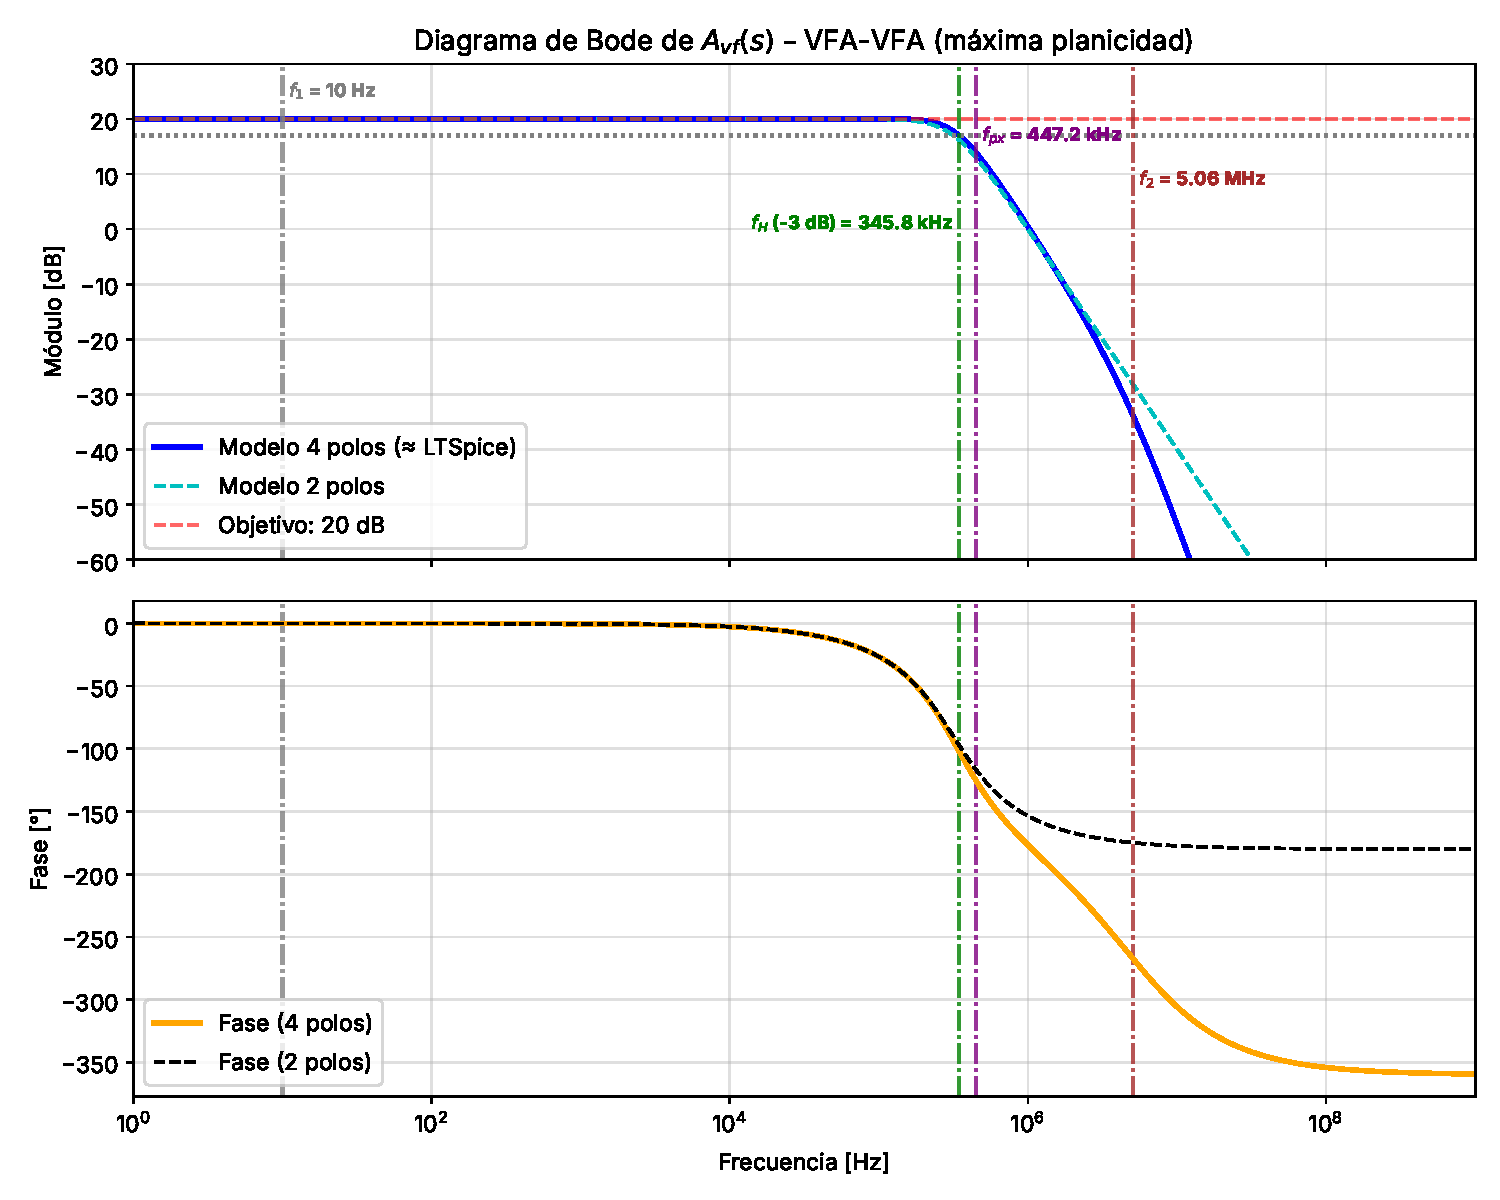
\includegraphics[width=0.95\linewidth,height=0.42\textheight,keepaspectratio]{Imagenes/c1_bode_lazo_cerrado.pdf}
    \caption{Diagrama de Bode a lazo cerrado (modelos de 2 y 4 polos). Se observa la ausencia de sobrepico, propia de MPM.}
    \label{fig:bode_lc_c1}
\end{figure}

\begin{figure}[H]
    \centering
    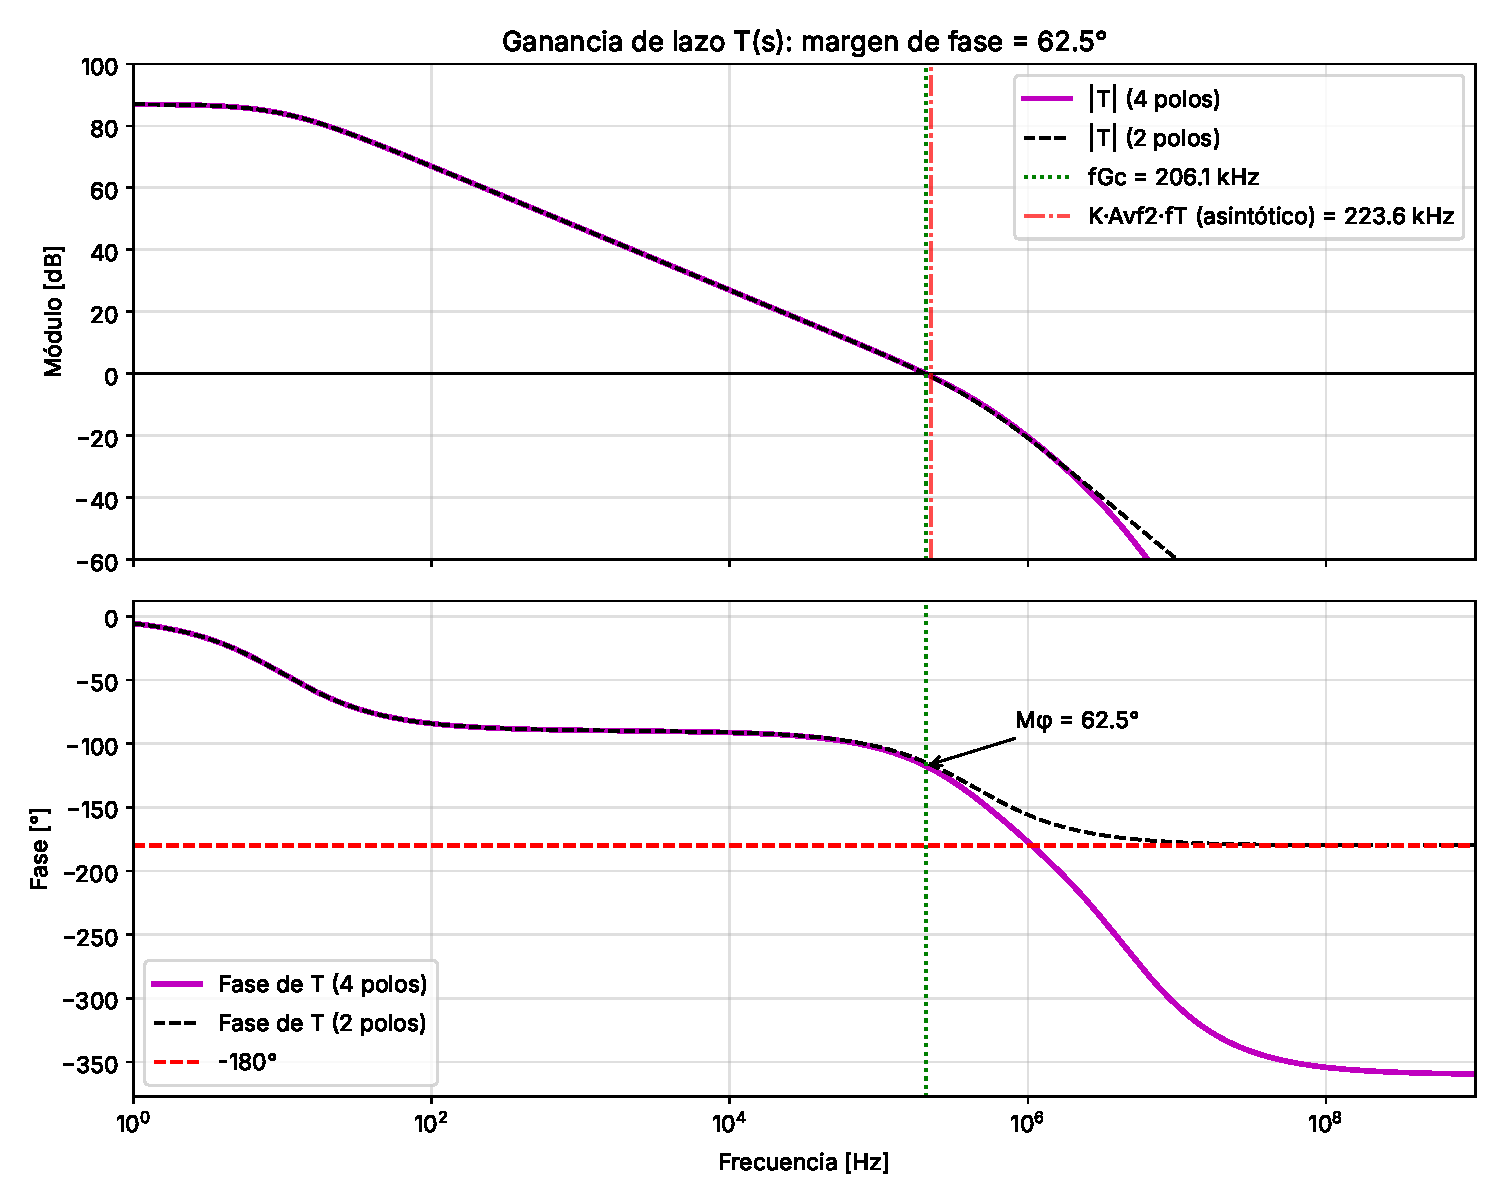
\includegraphics[width=0.95\linewidth,height=0.42\textheight,keepaspectratio]{Imagenes/c1_bode_ganancia_lazo.pdf}
    \caption{Diagrama de Bode de la ganancia de lazo: frecuencia crítica y margen de fase.}
    \label{fig:bode_lazo_c1}
\end{figure}

\paragraph{Respuesta al escalón teórica.} La \autoref{fig:escalon_teorico_c1} muestra la respuesta a un escalón de $0{,}1\text{ V}$ (salida de $1\text{ V}$) de los modelos de dos y de cuatro polos; los sobrepicos y el margen de fase estimado se comparan con la simulación en la \autoref{tab:escalon_c1}.

\begin{figure}[H]
    \centering
    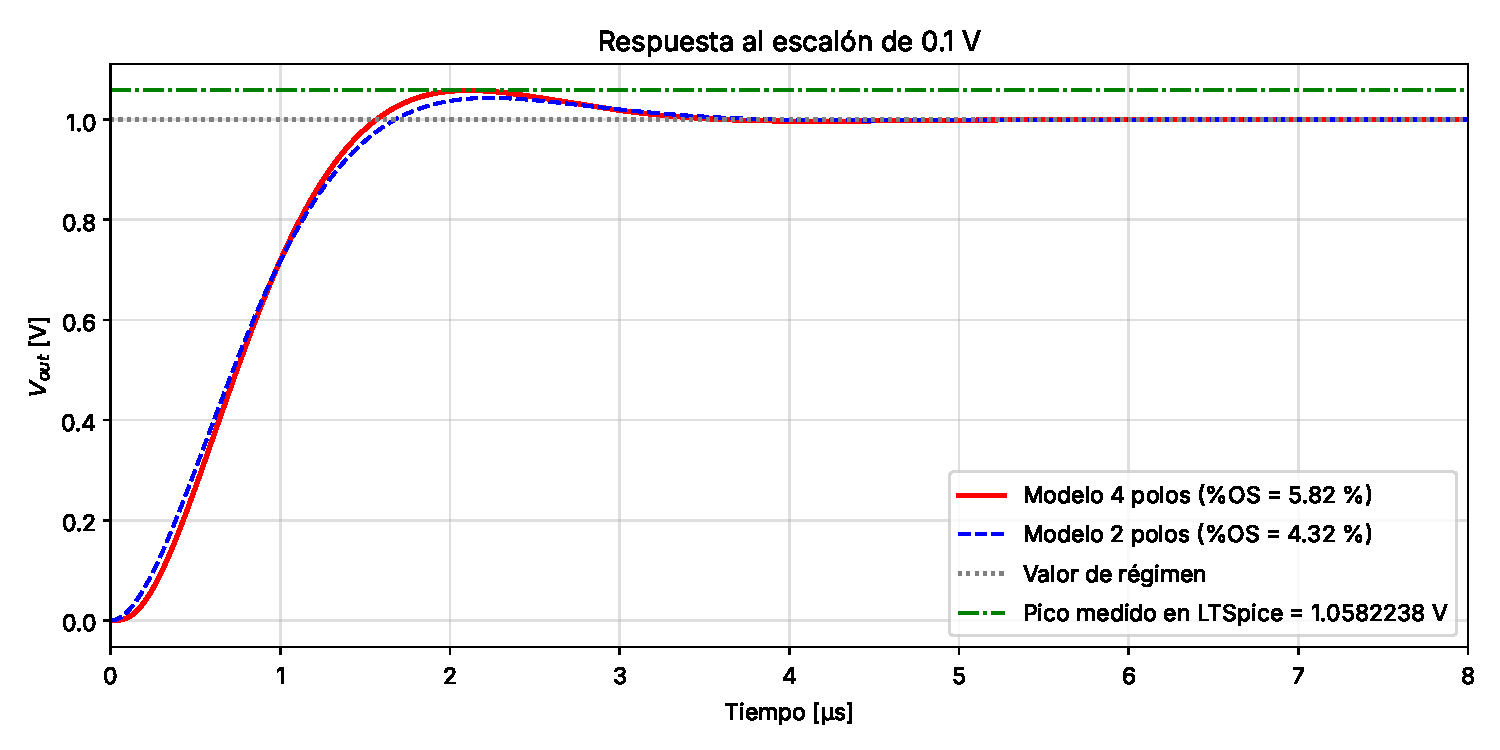
\includegraphics[width=0.95\linewidth,height=0.42\textheight,keepaspectratio]{Imagenes/c1_escalon_teorico.pdf}
    \caption{Respuesta al escalón teórica (2 y 4 polos).}
    \label{fig:escalon_teorico_c1}
\end{figure}

\subsection{Simulación}
\label{sec:simulacion_c1}

Se simularon en LTSpice los circuitos de la \autoref{fig:circuito_VFA_VFA}: lazo abierto, ganancia de lazo y lazo cerrado, con el modelo del LM324 de la bibliografía. En el esquemático la red global se implementó con $R_i = 1\text{ k}\Omega$ y $R_f = 9\text{ k}\Omega$ (misma relación que en el diseño), y la local con $R_1 = 10\text{ k}\Omega$ y $R_2 = 12{,}361\text{ k}\Omega$.

\begin{figure}[H]
    \centering
    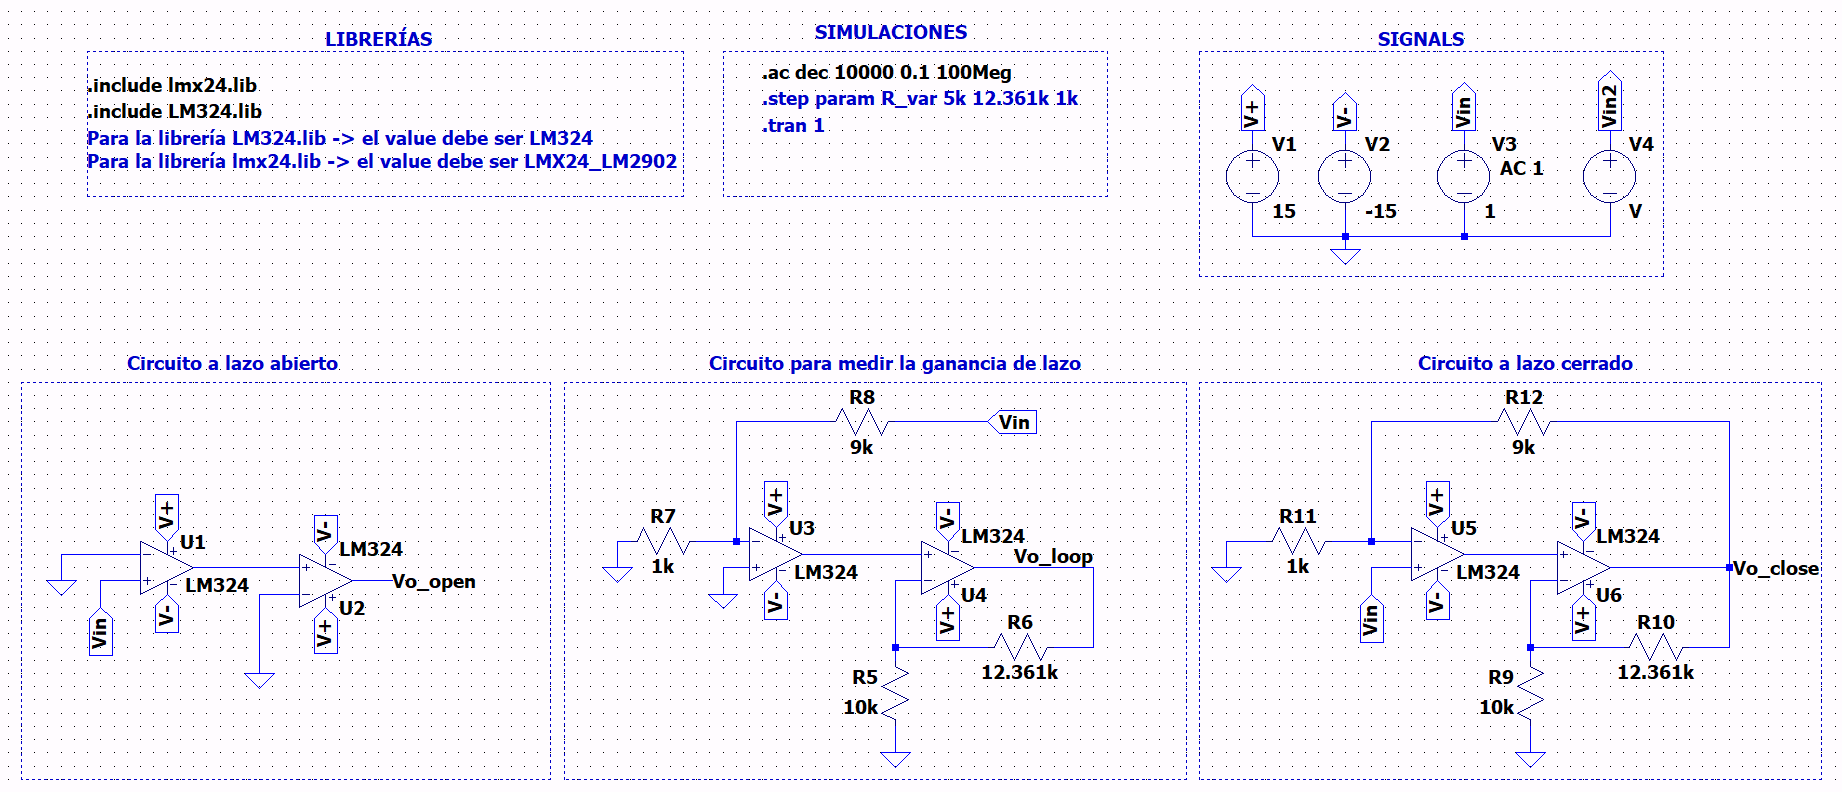
\includegraphics[width=\linewidth,height=0.32\textheight,keepaspectratio]{Imagenes/simulation_circuits_comp.png}
    \caption{Esquemático VFA-VFA, LTSpice.}
    \label{fig:circuito_VFA_VFA}
\end{figure}

\subsubsection{Respuesta en frecuencia a lazo abierto}
La \autoref{fig:rta_frec_open_loop_comp} muestra la respuesta a lazo abierto. Al tratarse de dos amplificadores idénticos en cascada, la ganancia en banda media es $A_{d0}^2$ ($200\text{ dB}$) y los polos son dobles, en $f_1 = 10\text{ Hz}$ y $f_2 = 5{,}06\text{ MHz}$.

\begin{figure}[H]
    \centering
    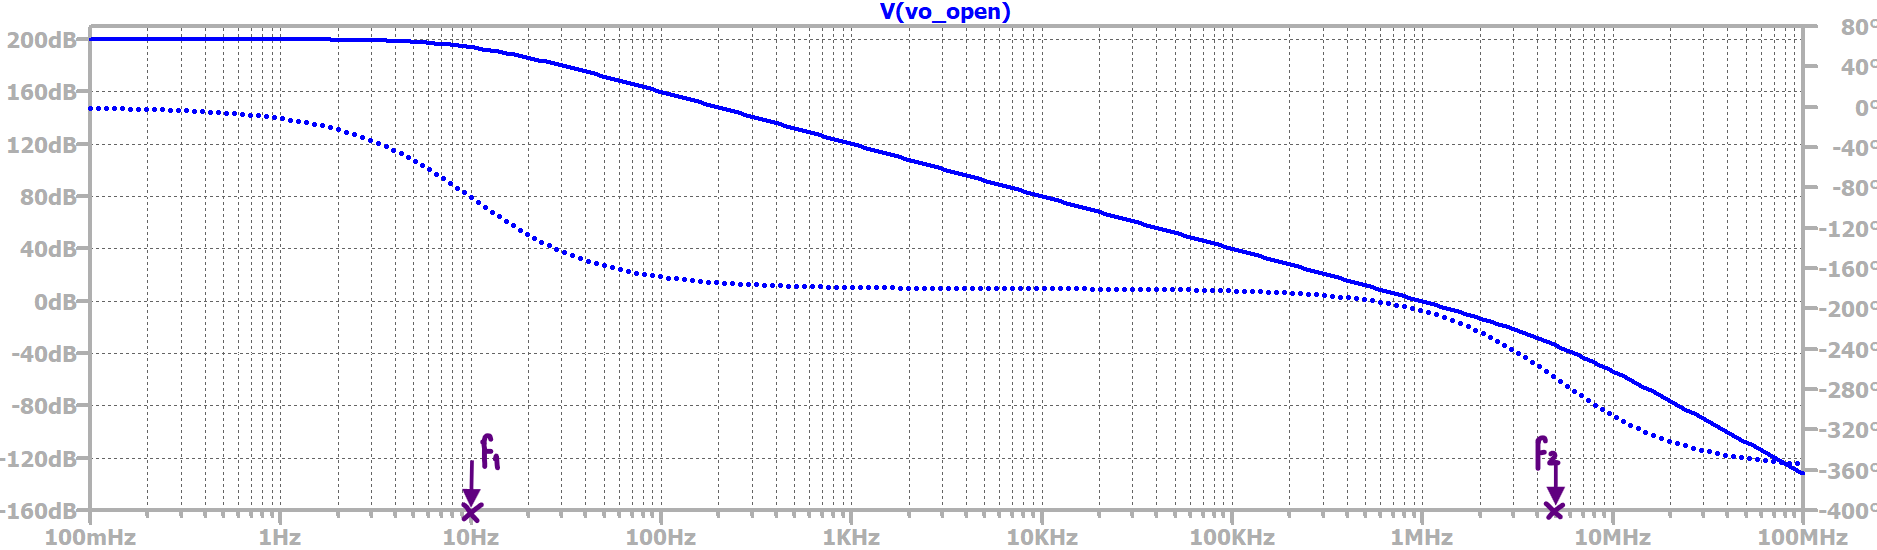
\includegraphics[width=\linewidth,height=0.32\textheight,keepaspectratio]{Imagenes/rta_frec_open_loop_comp.png}
    \caption{Respuesta en frecuencia a \textbf{lazo abierto}.}
    \label{fig:rta_frec_open_loop_comp}
\end{figure}

\subsubsection{Respuesta en frecuencia de la ganancia de lazo}
En la \autoref{fig:rta_frec_loop_comp.png} se midió con los cursores el punto de cruce de la ganancia de lazo, obteniéndose una frecuencia crítica $f_g \approx 206\text{ kHz}$ y un margen de fase $M_\varphi \approx 62{,}52^\circ$.

\begin{figure}[H]
    \centering
    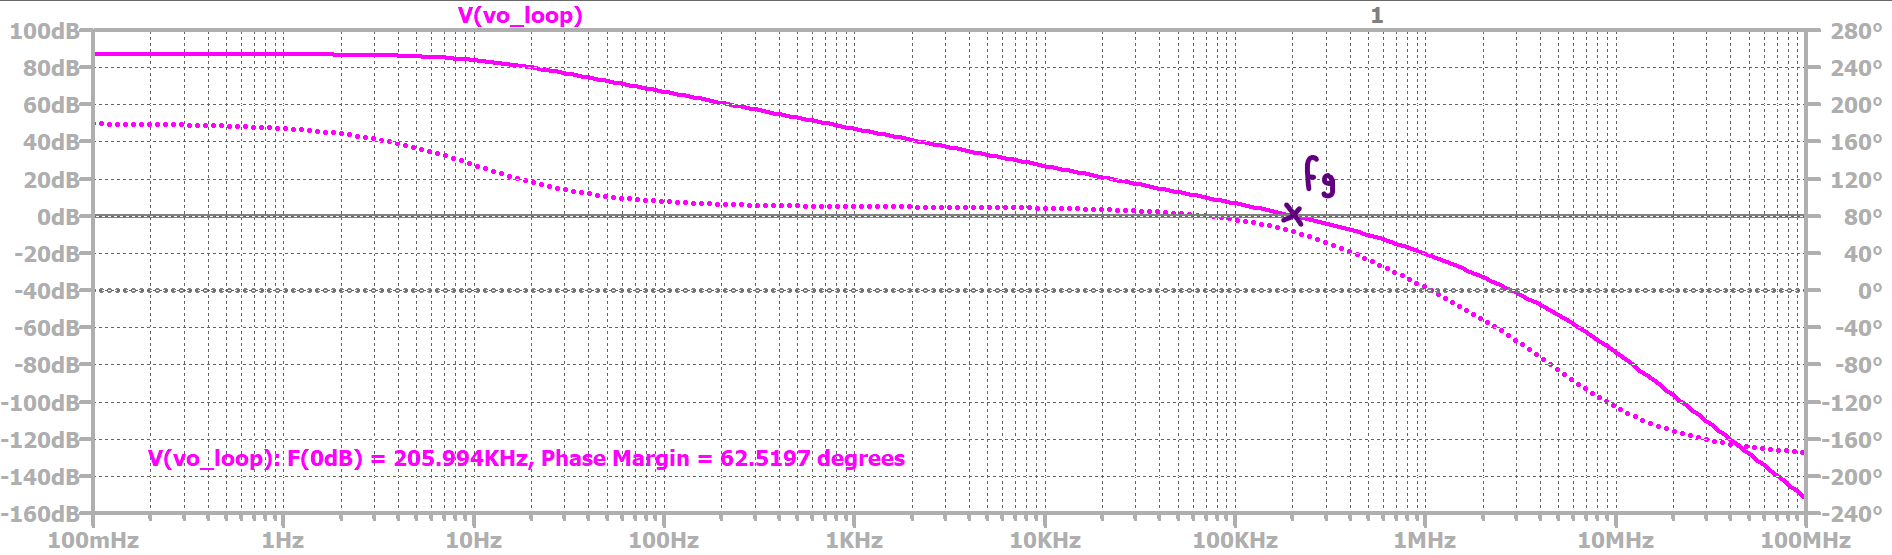
\includegraphics[width=\linewidth,height=0.32\textheight,keepaspectratio]{Imagenes/rta_frec_loop_comp.png}
    \caption{Respuesta en frecuencia de la \textbf{ganancia de lazo}.}
    \label{fig:rta_frec_loop_comp.png}
\end{figure}

\subsubsection{Respuesta en frecuencia a lazo cerrado}
La \autoref{fig:rta_frec_close_loop_BW_comp} confirma la ganancia en banda media de $20\text{ dB}$. El ancho de banda real medido, donde la ganancia cae $3\text{ dB}$ (a $17\text{ dB}$), es $f_H = 345\text{ kHz}$. La caída suave, sin sobrepico, valida la compensación por desplazamiento de polos.

\begin{figure}[H]
    \centering
    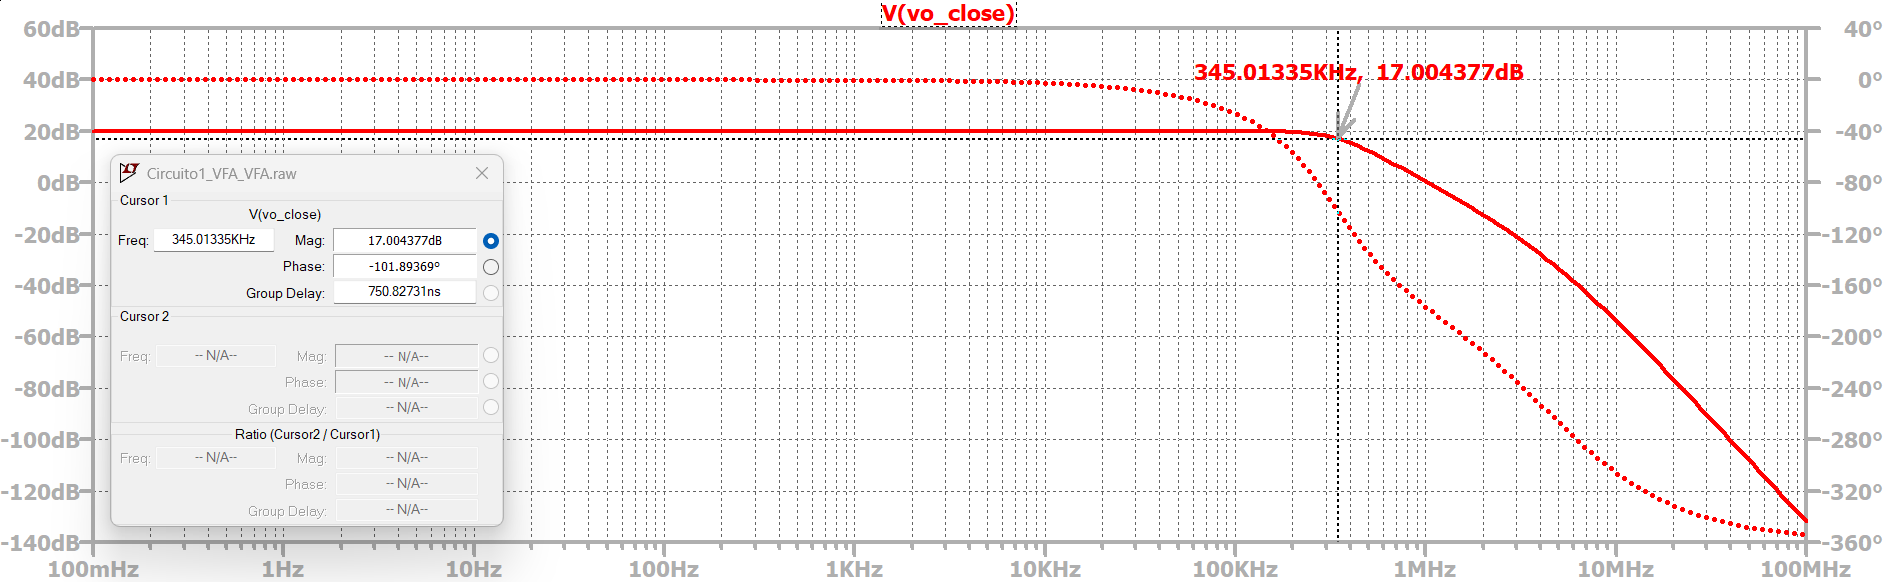
\includegraphics[width=\linewidth,height=0.32\textheight,keepaspectratio]{Imagenes/rta_frec_close_loop_BW_comp.png}
    \caption{Respuesta en frecuencia a \textbf{lazo cerrado}.}
    \label{fig:rta_frec_close_loop_BW_comp}
\end{figure}

\subsubsection{Respuesta al escalón}
Se aplicó un escalón de $0{,}1\text{ V}$ (salida de $1\text{ V}$), con tiempos de subida y de bajada de $10\text{ ns}$ y un paso máximo de simulación de $5\text{ ns}$. El flanco es mucho más rápido que el tiempo de subida del circuito ($\approx 1\,\mu\text{s}$), de modo que el sobrepico depende solo del circuito, y la amplitud pequeña evita que el \emph{slew rate} limite la respuesta. Se midieron $V_{pico} = 1{,}0582\text{ V}$ y $V_{estacionario} = 0{,}99995\text{ V}$. Aplicando las \autoref{eq:OS}, \autoref{eq:zeta} y \autoref{eq:MF_exacta} (\autoref{sec:escalon_mf}):
\begin{equation}
    \mathrm{\char37}OS = \frac{1{,}0582 - 0{,}99995}{0{,}99995}\cdot 100 = 5{,}83\,\mathrm{\char37}
\end{equation}
\begin{equation}
    \zeta = \frac{-\ln(0{,}0583)}{\sqrt{\pi^2 + \ln^2(0{,}0583)}} \approx 0{,}671
\end{equation}
\begin{equation}
    MF = \arctan\left( \frac{2\cdot 0{,}671}{\sqrt{\sqrt{1+4(0{,}671)^4}-2(0{,}671)^2}} \right) \approx 63{,}6^\circ
\end{equation}

\begin{figure}[H]
    \centering
    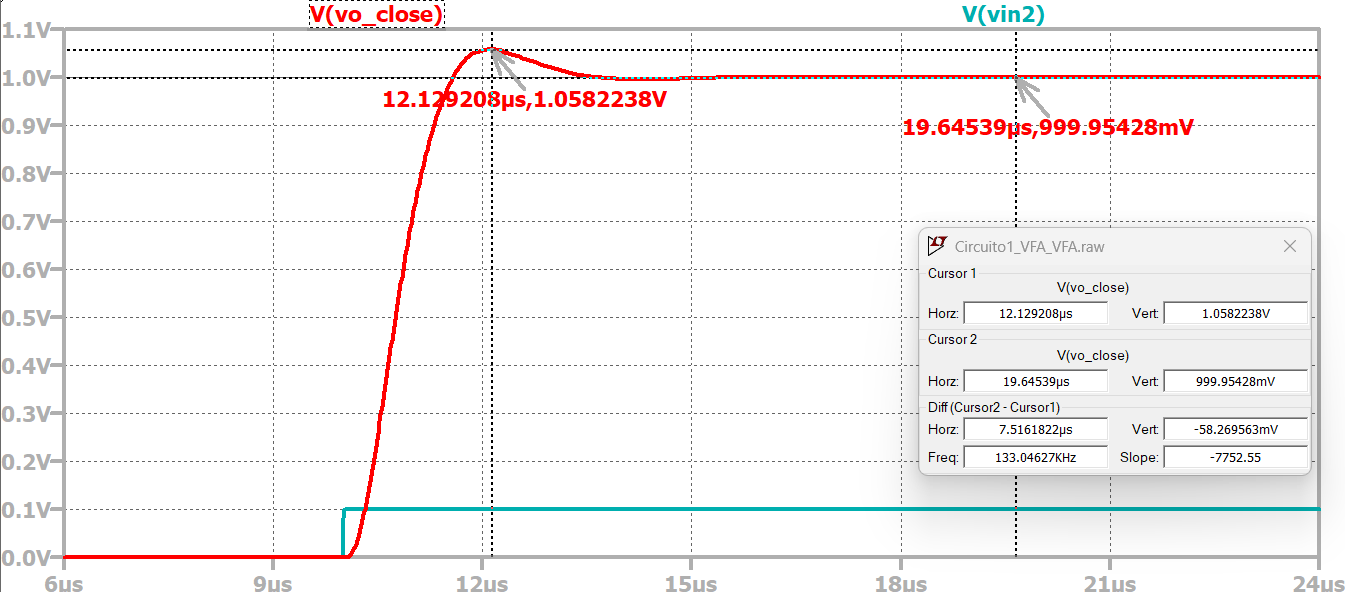
\includegraphics[width=\linewidth,height=0.32\textheight,keepaspectratio]{Imagenes/c1_rta_step.png}
    \caption{Respuesta al escalón de $\SI{0,1}{V}$ (LTSpice): $V_{pico} = \SI{1,0582}{V}$ y $V_{est} = \SI{0,99995}{V}$.}
    \label{fig:rta_step}
\end{figure}

\subsection{Comparación de resultados}
\label{sec:comparacion_c1}

La \autoref{tab:final_c1} compara los valores analíticos (dos polos), el modelo de cuatro polos y las mediciones de LTSpice.

\begin{table}[H]
\centering
\caption{Comparación entre teoría y simulación (VFA-VFA). Error $= (\text{teórico}-\text{LTSpice})/\text{LTSpice}$.}
\label{tab:final_c1}
\small
\setlength{\tabcolsep}{4pt}
\begin{tabularx}{\textwidth}{>{\raggedright\arraybackslash}X c c c c c}
\toprule
\textbf{Magnitud} & \textbf{Analítico} & \textbf{4 polos} & \textbf{LTSpice} & \textbf{Err. anal. [\%]} & \textbf{Err. 4p [\%]} \\
\midrule
Ancho de banda potencial $f_G$ [kHz] & 316,2 & --- & --- & --- & --- \\
Cruce de $T$ asintótico $f_{Gc}$ [kHz] & 223,6 & 206,1 & 206,0 & $+8{,}6$ & $0{,}0$ \\
Cruce de $T$ exacto (2 polos) [kHz] & 203,5 & 206,1 & 206,0 & $-1{,}2$ & $0{,}0$ \\
Margen de fase del lazo [$^\circ$] & 65,53 & 62,51 & 62,52 & $+4{,}8$ & $0{,}0$ \\
Frecuencia de polos $f_p$ [kHz] & 316,2 & 330,3 & --- & --- & --- \\
Ancho de banda real $f_H$ [kHz] & 316,2 & 345,8 & 345,0 & $-8{,}3$ & $+0{,}2$ \\
Sobrepico \%OS [\%] & 4,32 & 5,82 & 5,83 & $-25{,}8$ & $-0{,}1$ \\
$M_\varphi$ desde el escalón [$^\circ$] & 65,53 & 63,57 & 63,56 & $+3{,}1$ & $0{,}0$ \\
\bottomrule
\end{tabularx}
\end{table}

\begin{table}[H]
\centering
\caption{Respuesta al escalón de $0{,}1\text{ V}$ y margen de fase estimado.}
\label{tab:escalon_c1}
\begin{tabular}{lccc}
\toprule
\textbf{Magnitud} & \textbf{2 polos} & \textbf{4 polos} & \textbf{LTSpice} \\
\midrule
$V_{pico}$ [V] & 1,043 & 1,058 & 1,058 \\
$V_{est}$ [V] & 1,000 & 1,000 & 1,000 \\
$\mathrm{\char37}OS$ & 4,32 & 5,82 & 5,83 \\
$\zeta$ & 0,7071 & 0,6711 & 0,6709 \\
$M_\varphi$ estimado [$^\circ$] & 65,53 & 63,57 & 63,56 \\
\bottomrule
\end{tabular}
\end{table}


\subsection{Análisis y conclusión parcial}
\label{sec:concl_c1}

\begin{itemize}
    \item El modelo de dos polos predice un $f_H = f_G = 316{,}2\text{ kHz}$; el modelo de cuatro polos y la simulación dan $\approx 345\text{ kHz}$. La diferencia ($\approx 9\,\mathrm{\char37}$) se debe al segundo polo del LM324 ($f_2$), no incluido en el modelo simple, que eleva ligeramente $Q$ ($0{,}746$) y el ancho de banda.
    \item La frecuencia crítica y el margen de fase medidos en LTSpice ($206{,}0\text{ kHz}$, $62{,}52^\circ$) coinciden con el modelo de cuatro polos (error menor a $0{,}1\,\mathrm{\char37}$), lo que valida el modelo. Respecto del modelo de dos polos el margen de fase es $\approx 3^\circ$ menor, consecuencia del segundo polo.
    \item El margen de fase estimado a partir del escalón ($63{,}6^\circ$) es consistente con el medido en el lazo ($62{,}5^\circ$), con una diferencia de $\approx 1^\circ$; la relación entre sobrepico y margen de fase es aproximada, pues el sistema no es exactamente de segundo orden.
    \item El sobrepico simulado ($5{,}83\,\mathrm{\char37}$) coincide con el del modelo de cuatro polos ($5{,}82\,\mathrm{\char37}$), y es mayor que el del modelo de dos polos ($4{,}32\,\mathrm{\char37}$): el segundo polo del LM324 aumenta el sobrepico. La medición se hizo con un escalón de $0{,}1\text{ V}$ y flancos de $10\text{ ns}$; con un escalón de $1\text{ V}$ (salida de $10\text{ V}$) el sobrepico medido fue menor ($4{,}8\,\mathrm{\char37}$), posiblemente por la limitación de velocidad de respuesta (\emph{slew rate}) del modelo y por el flanco de esa simulación, por lo que no era representativa de pequeña señal.
    \item Se verifica el diseño: ganancia de $20\text{ dB}$, respuesta sin sobrepico en frecuencia y margen de fase cercano a $65^\circ$ (MPM), con un ancho de banda real $\approx 3{,}4$ veces el del amplificador simple ($f_T/A_{vf} = 100\text{ kHz}$).
\end{itemize}

\section{Desarrollo: Caso 2, configuración VFA-CFA}
\label{sec:desarrollo_c2}

\subsection{Diseño}
\label{sec:diseno_c2}

El compuesto combina el LM324 como $A_{01}$ (VFA), que aporta la precisión en continua, con el LM6181 como $A_{02}$ (CFA), que aporta la velocidad. Ambos operan en configuración no inversora y el CFA queda dentro del lazo global: la ganancia total la fija la red $R_i$--$R_f$ y la ganancia local del CFA, $A_{vfi2}$, la red $R_1$--$R_2$. Se busca un ancho de banda potencial $f_g \approx \SI{2}{MHz}$ con una respuesta cercana a MPM, teniendo en cuenta el segundo polo del VFA.

\paragraph{Ganancia del CFA.} Según la \autoref{sec:compuesto_distinto}, el ancho de banda potencial fija la ganancia local del CFA (\autoref{eq:wg_VFACFA}), y la condición de MPM impone una cota superior (\autoref{eq:Avfi2_max}):
\begin{gather}
    A_{vfi2} = \frac{f_g}{K\,f_T} = \frac{\SI{2}{MHz}}{0{,}1\cdot\SI{1}{MHz}} = 20 \\
    A_{vfi2,max} = \frac{f_2}{2\,K\,f_T} = \frac{\SI{5,06}{MHz}}{2\cdot 0{,}1\cdot\SI{1}{MHz}} = 25{,}3
\end{gather}
Se adopta $A_{vfi2} = 20 < A_{vfi2,max}$. Con este valor $Q_p^2 = f_g/f_2 = 0{,}395$ (\autoref{eq:Qp_VFACFA}), es decir, una respuesta algo más amortiguada que MPM ($Q_p^2 = 1/2$), lo que deja margen para el atraso de fase que agregan los polos del CFA.

\paragraph{Red local del CFA.} Se toma $R_2 = \SI{820}{\ohm}$ (valor recomendado por el fabricante) y $r_i = \SI{20}{\ohm}$ (supuesto, pues el fabricante no lo publica). Resulta
\begin{gather}
    R_1 = \frac{R_2}{A_{vfi2}-1} = \frac{820}{19} = \SI{43,16}{\ohm} \\
    R_{eff} = R_2 + r_i\,A_{vfi2} = 820 + 20\cdot 20 = \SI{1220}{\ohm} \\
    f_{cfa} = \frac{1}{2\pi\,C_t\,R_{eff}} = \SI{27,2}{MHz}
\end{gather}
El polo del CFA queda $14$ veces por encima de $f_g$ y el margen de fase del CFA aislado es $\ang{72,5}$ (\autoref{eq:Mphi_CFA}), por lo que el valor elegido de $R_2$ es estable. La \autoref{tab:parametros_vfa_cfa} reúne el diseño completo.

\begin{table}[H]
\centering
\caption{Diseño VFA-CFA: expresiones, cálculo y valores.}
\label{tab:parametros_vfa_cfa}
\footnotesize
\setlength{\tabcolsep}{4pt}
\begin{tabular}{>{\raggedright\arraybackslash}p{0.31\textwidth} >{\centering\arraybackslash}p{0.2\textwidth} >{\centering\arraybackslash}p{0.27\textwidth} >{\centering\arraybackslash}p{0.13\textwidth}}
\toprule
\textbf{Parámetro} & \textbf{Expresión} & \textbf{Cálculo} & \textbf{Valor} \\
\midrule
Ganancia global $A_{vf}$ & dato & \SI{20}{dB} & \SI{10}{V/V} \\
Factor de realimentación $K$ & $1/A_{vf}$ & $1/10$ & \num{0,1} \\
Resistencia de entrada global $R_i$ & elegida & --- & \SI{1}{k\ohm} \\
Resistencia de realimentación global $R_f$ & $R_i(A_{vf}-1)$ & $1\text{ k}\Omega\cdot 9$ & \SI{9}{k\ohm} \\
Ganancia del CFA $A_{vfi2}$ & $f_g/(K f_T)$ & $2\text{ MHz}/(0{,}1\cdot 1\text{ MHz})$ & \SI{20}{V/V} \\
Cota de MPM $A_{vfi2,max}$ & $f_2/(2Kf_T)$ & $5{,}06\text{ MHz}/0{,}2\text{ MHz}$ & \SI{25,3}{V/V} \\
Realimentación local $R_2$ & elegida (fabricante) & --- & \SI{820}{\ohm} \\
Resistencia local a tierra $R_1$ & $R_2/(A_{vfi2}-1)$ & $820/19$ & \SI{43,16}{\ohm} \\
Resistencia efectiva $R_{eff}$ & $R_2 + r_iA_{vfi2}$ & $820 + 20\cdot 20$ & \SI{1220}{\ohm} \\
Polo del CFA $f_{cfa}$ & $1/(2\pi C_tR_{eff})$ & --- & \SI{27,2}{MHz} \\
Ganancia de lazo en continua $T_0$ & $K\,A_{d0}\,A_{vfi2}$ & $0{,}1\cdot 10^5\cdot 20$ & \num{200000} (\SI{106}{dB}) \\
Separación de polos $D_p$ & $f_2/f_1$ & $5{,}06\text{ MHz}/10\text{ Hz}$ & \num{506000} \\
\bottomrule
\end{tabular}
\end{table}

\subsection{Resultados analíticos}
\label{sec:analitico_c2}

Con $T(s)\cong T_0/[(1+s/\omega_1)(1+s/\omega_2)]$ y las relaciones de la \autoref{sec:mpm} se obtienen los valores de la \autoref{tab:analitica_c2}. Los polos de lazo cerrado son $s^2 + (\omega_1+\omega_2)s + \omega_1\omega_2(1+T_0) = 0$, y el margen de fase se calcula sobre el cruce exacto de $|T|=1$; el resultado coincide con la fórmula del apunte $M_\varphi = 90^\circ - \arctan(\Omega_GQ_p)$, que vale para cualquier $Q_p$ (\autoref{eq:omegaG}).

\begin{table}[H]
\centering
\caption{Resultados analíticos (modelo de dos polos), Caso 2.}
\label{tab:analitica_c2}
\small
\setlength{\tabcolsep}{4pt}
\begin{tabular}{>{\raggedright\arraybackslash}p{0.37\textwidth} >{\centering\arraybackslash}p{0.31\textwidth} >{\centering\arraybackslash}p{0.2\textwidth}}
\toprule
\textbf{Magnitud} & \textbf{Expresión} & \textbf{Valor} \\
\midrule
Ancho de banda potencial $f_g$ & $K\,A_{vfi2}\,f_T$ & \SI{2,000}{MHz} \\
Cruce exacto de $T$, $f_{Gc}$ & $|T(jf)|=1$ & \SI{1,875}{MHz} \\
$\Omega_G = f_{Gc}/f_p$ & --- & \num{0,5895} \\
Margen de fase $M_\varphi$ & \autoref{eq:Mphi_2polos} & \ang{69,66} \\
Frecuencia de los polos $f_p$ & $\sqrt{\omega_1\omega_2(1+T_0)}/2\pi$ & \SI{3,181}{MHz} \\
Factor de calidad $Q_p$ & $\omega_p/(\omega_1+\omega_2)$ & \num{0,629} \\
Amortiguamiento $\zeta$ & $1/(2Q_p)$ & \num{0,795} \\
Polos de lazo cerrado & $s_{1,2}$ & $(-2{,}530 \pm j\,1{,}929)$ MHz \\
Ancho de banda real $f_H$ ($-3$ dB) & $f_p\sqrt{a+\sqrt{a^2+1}}$ & \SI{2,791}{MHz} \\
\bottomrule
\end{tabular}
\end{table}

Como $Q_p<1/\sqrt2$, la respuesta es más amortiguada que MPM; el ancho de banda real ($\SI{2,79}{MHz}$) resulta mayor que el potencial ($f_g=\SI{2}{MHz}$), igual que en el Caso 1.

Para incluir el efecto del CFA se armó el modelo de cuatro polos, con el CFA realimentado de la \autoref{eq:Avf_CFA_ri} y $Z_t$ de dos polos. Sus resultados se comparan en la \autoref{tab:modelos_c2}. El CFA agrega atraso de fase, por lo que el margen de fase baja respecto del modelo simple, y eleva el $Q_p$ y el ancho de banda.

\begin{table}[H]
\centering
\caption{Resultados numéricos: modelo de 2 polos y de 4 polos, Caso 2.}
\label{tab:modelos_c2}
\begin{tabular}{lcc}
\toprule
\textbf{Magnitud} & \textbf{2 polos} & \textbf{4 polos} \\
\midrule
Frecuencia crítica $f_{Gc}$ [MHz] & 1,875 & 1,873 \\
Margen de fase [$^\circ$] & 69,66 & 65,74 \\
Margen de ganancia [dB] & $\infty$ & 23,2 \\
Ancho de banda real ($-3$ dB) [MHz] & 2,791 & 3,039 \\
Frecuencia de los polos $f_p$ [MHz] & 3,181 & 3,165 \\
Factor de calidad $Q_p$ & 0,629 & 0,681 \\
Polos dominantes [MHz] & $-2{,}530 \pm j\,1{,}929$ & $-2{,}322 \pm j\,2{,}150$ \\
\bottomrule
\end{tabular}
\end{table}

\emph{Nota:} el margen de ganancia del modelo de dos polos es infinito porque la fase de $T(s)$ tiende asintóticamente a $-180^\circ$ sin alcanzarlo a ninguna frecuencia finita; con cuatro polos la fase sí cruza $-180^\circ$ y el margen de ganancia es finito.

\begin{figure}[H]
    \centering
    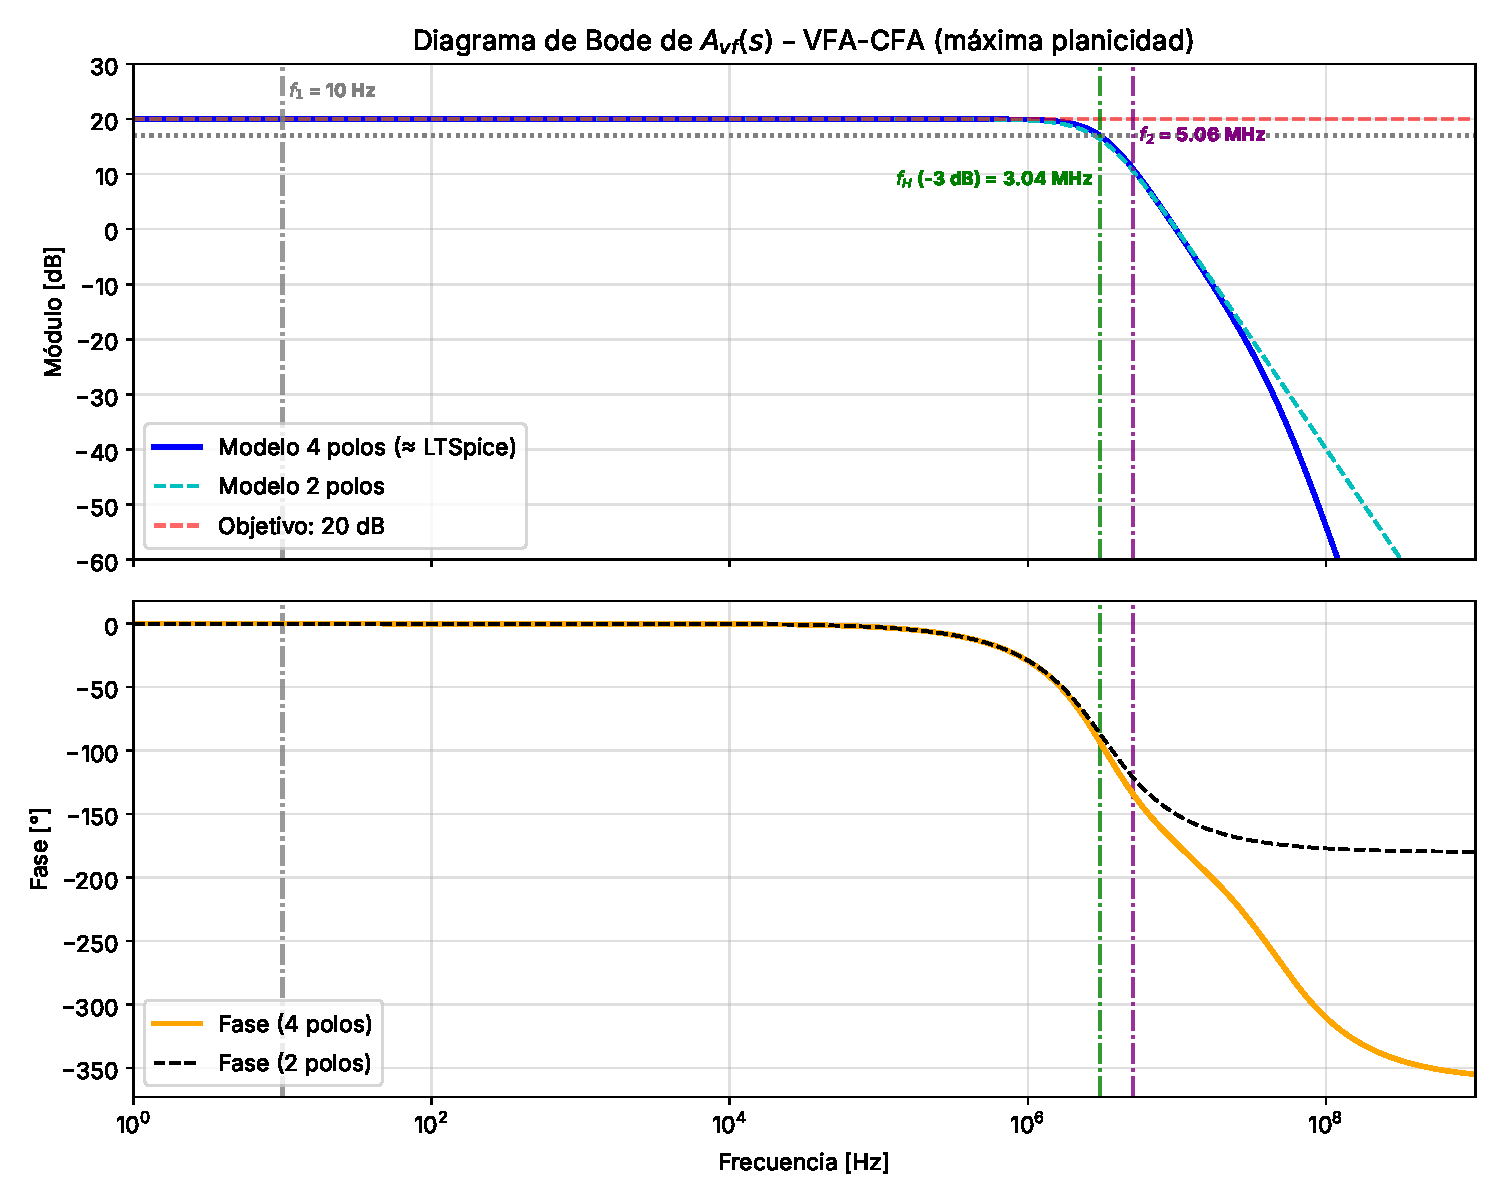
\includegraphics[width=0.95\linewidth,height=0.42\textheight,keepaspectratio]{Imagenes/c2_bode_lazo_cerrado.pdf}
    \caption{Diagrama de Bode a lazo cerrado (modelos de 2 y 4 polos), Caso 2.}
    \label{fig:bode_lc_c2}
\end{figure}

\begin{figure}[H]
    \centering
    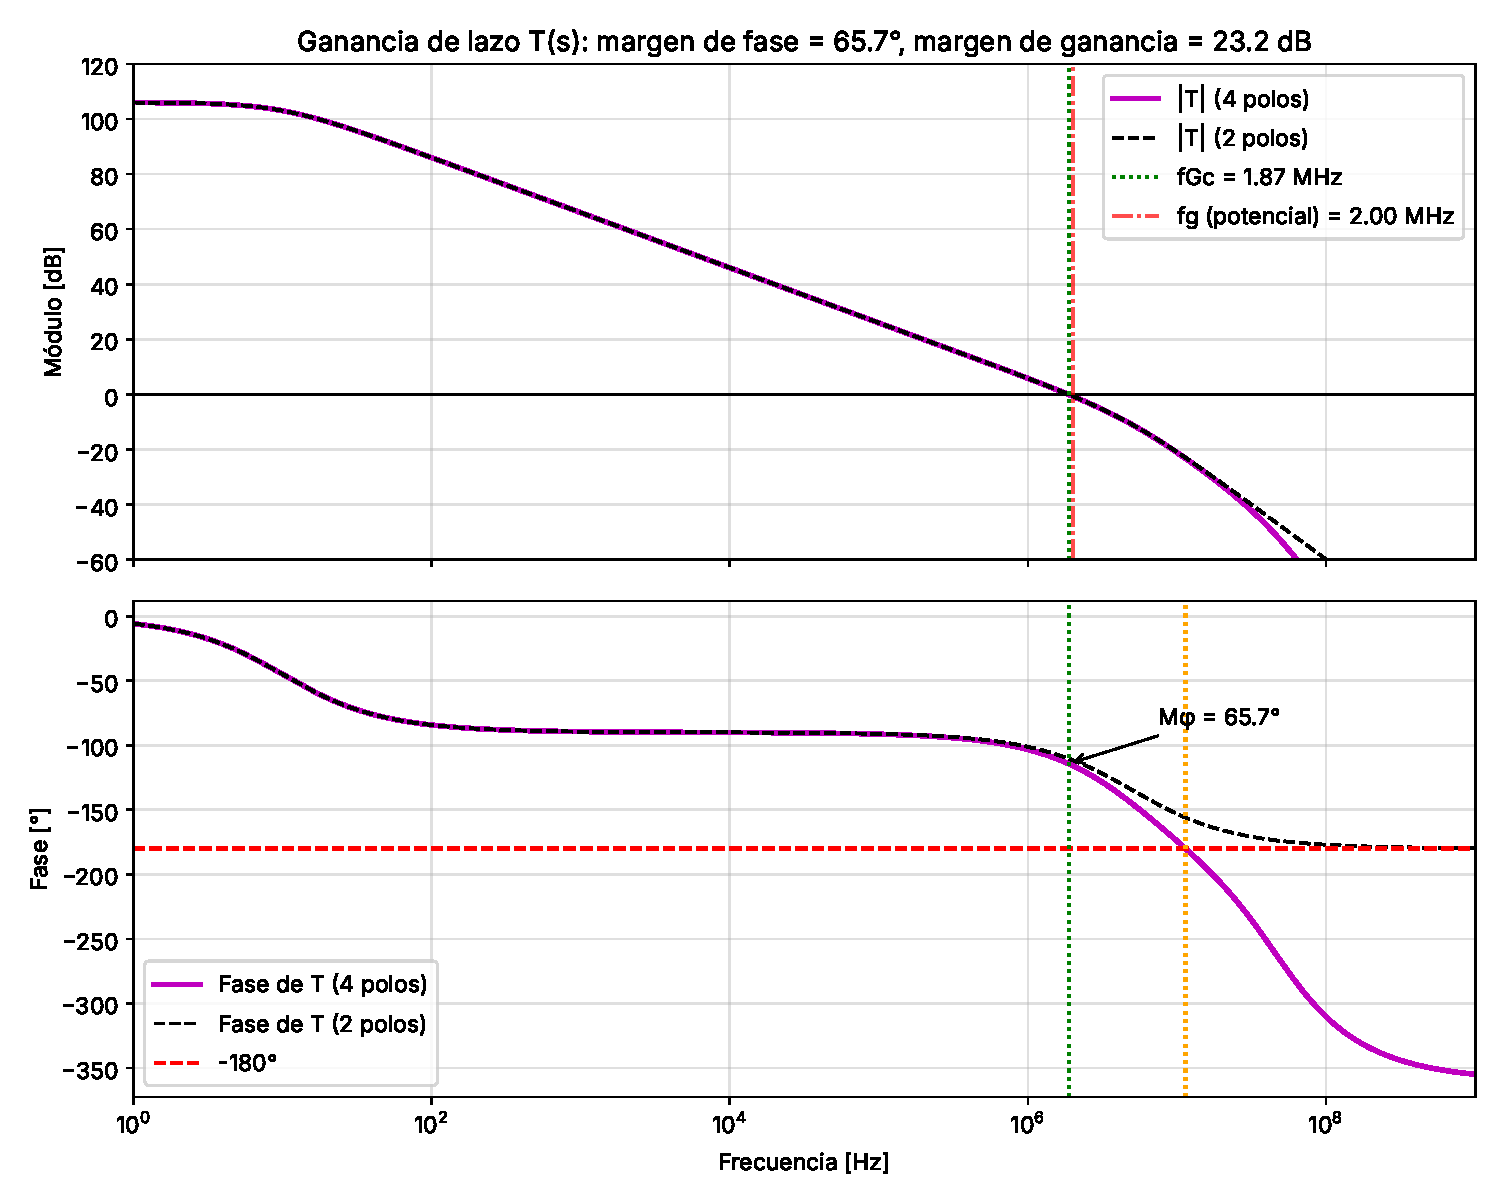
\includegraphics[width=0.95\linewidth,height=0.42\textheight,keepaspectratio]{Imagenes/c2_bode_ganancia_lazo.pdf}
    \caption{Diagrama de Bode de la ganancia de lazo, Caso 2: frecuencia crítica y margen de fase.}
    \label{fig:bode_lazo_c2}
\end{figure}

\paragraph{Sensibilidad al valor de $r_i$.} Como $r_i$ no está publicado, se repitió el modelo de cuatro polos para distintos valores (\autoref{tab:ri_c2}). El margen de fase varía menos de $3^\circ$ entre $r_i\approx0$ y $\SI{50}{\ohm}$, por lo que el supuesto no es crítico.

\begin{table}[H]
\centering
\caption{Sensibilidad al valor de $r_i$ (modelo de 4 polos), Caso 2.}
\label{tab:ri_c2}
\begin{tabular}{cccccc}
\toprule
$r_i$ [$\Omega$] & $R_{eff}$ [$\Omega$] & $f_{Gc}$ [MHz] & $M_\varphi$ [$^\circ$] & $M_G$ [dB] & BW [MHz] \\
\midrule
0 & 820 & 1,875 & 67,0 & 26,2 & 2,962 \\
10 & 1020 & 1,874 & 66,4 & 24,5 & 3,001 \\
20 & 1220 & 1,873 & 65,7 & 23,2 & 3,039 \\
30 & 1420 & 1,872 & 65,1 & 22,1 & 3,075 \\
50 & 1820 & 1,869 & 63,9 & 20,4 & 3,142 \\
\bottomrule
\end{tabular}
\end{table}

\paragraph{Respuesta al escalón teórica.} La \autoref{fig:escalon_teorico_c2} muestra la respuesta a un escalón de $\SI{0,1}{V}$ (salida de $\SI{1}{V}$) de los modelos de dos y de cuatro polos; los valores de sobrepico y margen de fase estimado se comparan con la simulación en la \autoref{tab:escalon_c2}.

\begin{figure}[H]
    \centering
    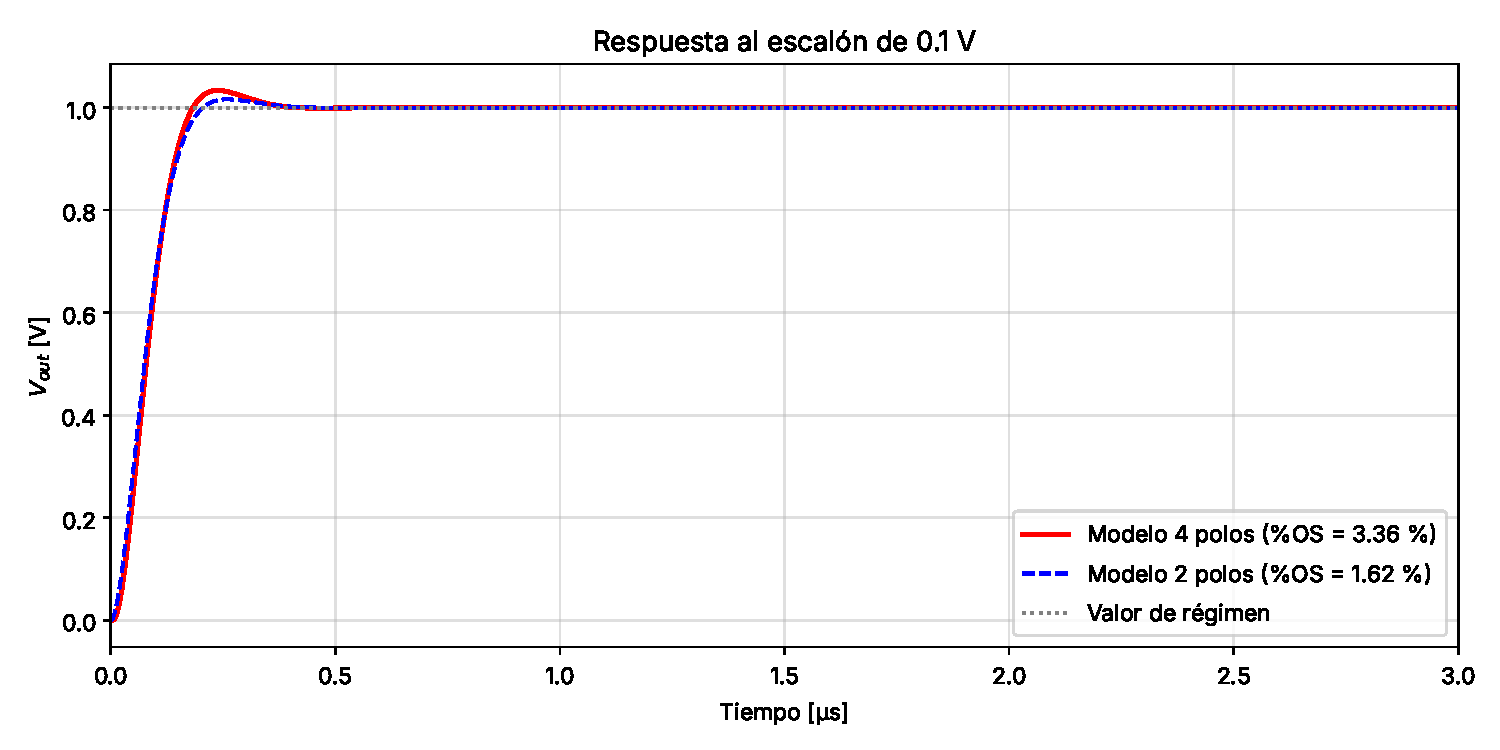
\includegraphics[width=0.95\linewidth,height=0.42\textheight,keepaspectratio]{Imagenes/c2_escalon_teorico.pdf}
    \caption{Respuesta al escalón teórica (2 y 4 polos), Caso 2.}
    \label{fig:escalon_teorico_c2}
\end{figure}

\subsection{Simulación}
\label{sec:simulacion_c2}

Se simularon en LTSpice los circuitos de lazo abierto, ganancia de lazo y lazo cerrado del compuesto VFA-CFA, con los modelos del LM324 (con la etapa de salida de adaptación de impedancia) y del LM6181. El esquemático usa $R_i = \SI{1}{k\ohm}$, $R_f = \SI{9}{k\ohm}$, $R_2 = \SI{820}{\ohm}$ y $R_1 = \SI{43,2}{\ohm}$.

\begin{figure}[H]
    \centering
    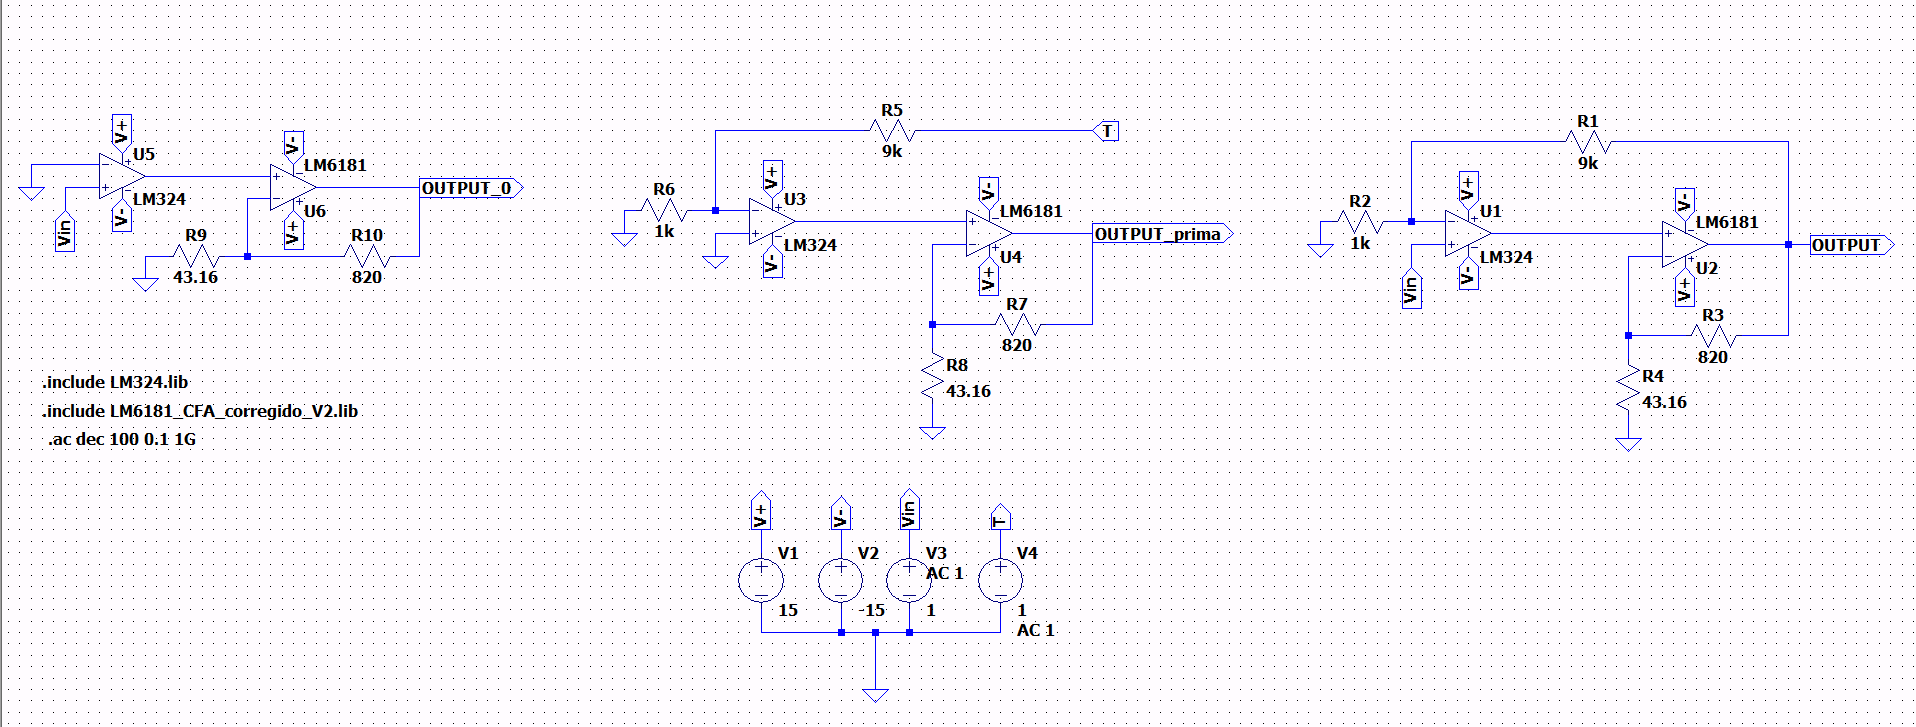
\includegraphics[width=1.0\linewidth,height=0.32\textheight,keepaspectratio]{Imagenes/c2_sim_circuitos.png}
    \caption{Esquemático VFA-CFA en LTSpice: lazo abierto (izquierda), ganancia de lazo (centro) y lazo cerrado (derecha).}
    \label{fig:circuito_VFA_CFA}
\end{figure}

\subsubsection{Respuesta en frecuencia a lazo abierto}
La \autoref{fig:rta_frec_open_loop_c2} muestra una ganancia en banda media de $A_{d0}A_{vfi2} = 100\text{ dB} + 26\text{ dB} = 126\text{ dB}$, con el primer polo en $f_1=\SI{10}{Hz}$ y pendiente $-20$ dB/dec hasta que actúan el segundo polo del VFA ($f_2$) y los del CFA.

\begin{figure}[H]
    \centering
    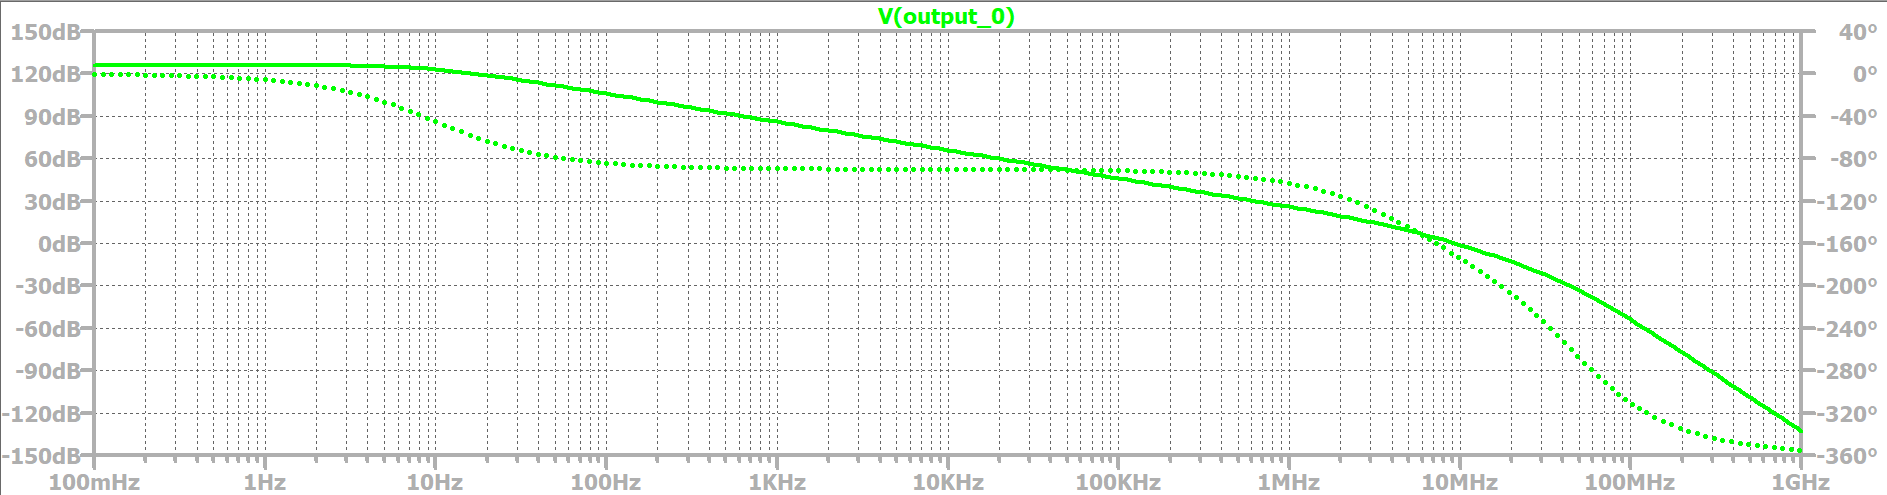
\includegraphics[width=0.95\linewidth,height=0.32\textheight,keepaspectratio]{Imagenes/c2_sim_lazo_abierto.png}
    \caption{Respuesta en frecuencia a \textbf{lazo abierto} del compuesto (módulo y fase).}
    \label{fig:rta_frec_open_loop_c2}
\end{figure}

\subsubsection{Respuesta en frecuencia de la ganancia de lazo}
Con los cursores sobre la curva de $-T$ (\texttt{V(output\_prima)}) se midió el cruce por \SI{0}{dB} en $f_{Gc} = \SI{1,873}{MHz}$, donde la fase es $M_\varphi = \ang{65,78}$ (el modelo de 4 polos predice \SI{1,873}{MHz} y \ang{65,74}). La ganancia de lazo en continua es de \SI{106}{dB}, con el polo dominante en \SI{10}{Hz}, y la curva a lazo abierto del compuesto (\texttt{V(output\_0)}) da \SI{126}{dB}, es decir $T_0 + 20\,\mathrm{dB}$, como corresponde a $T = K\,A$.

\begin{figure}[H]
    \centering
    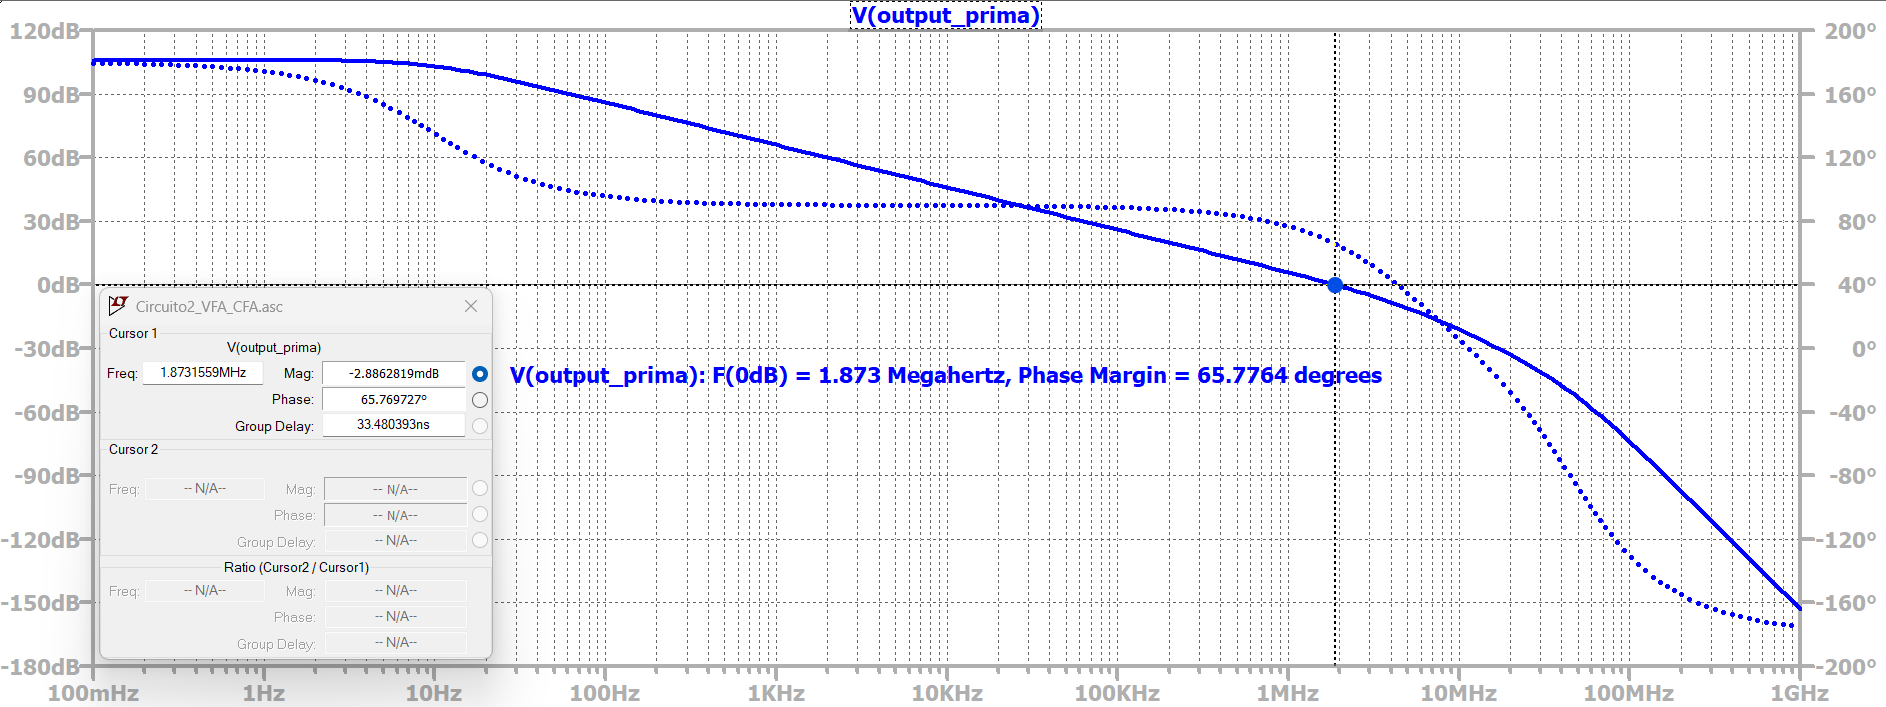
\includegraphics[width=0.95\linewidth,height=0.32\textheight,keepaspectratio]{Imagenes/c2_sim_lazo_T.png}
    \caption{Respuesta en frecuencia de la \textbf{ganancia de lazo} ($-T$): $f_{Gc} = \SI{1,873}{MHz}$ y $M_\varphi = \ang{65,78}$.}
    \label{fig:rta_frec_loop_c2}
\end{figure}

\subsubsection{Respuesta en frecuencia a lazo cerrado}
La \autoref{fig:rta_frec_close_loop_c2} confirma la ganancia en banda media de $\SI{20}{dB}$ ($\SI{19,9999}{dB}$ a $\SI{38,8}{kHz}$), sin sobrepico. Con el cursor a $\SI{17}{dB}$ se obtuvo $\SI{16,949}{dB}$ a $\SI{3,052}{MHz}$ ($-3{,}05$ dB respecto de banda media); interpolando al punto de $-3{,}01$ dB resulta un ancho de banda real $f_H \approx \SI{3,04}{MHz}$ (el modelo de cuatro polos predice $\SI{3,039}{MHz}$).

\begin{figure}[H]
    \centering
    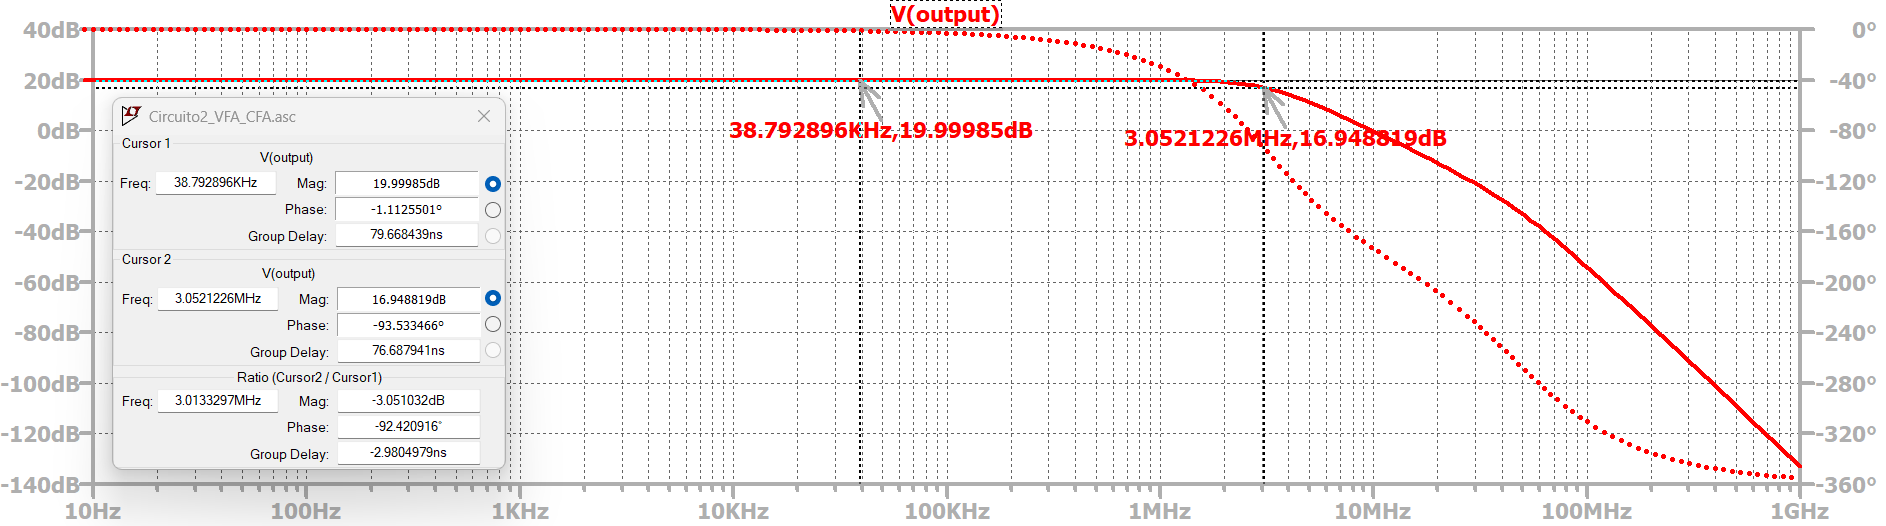
\includegraphics[width=0.95\linewidth,height=0.32\textheight,keepaspectratio]{Imagenes/c2_sim_lazo_cerrado.png}
    \caption{Respuesta en frecuencia a \textbf{lazo cerrado}.}
    \label{fig:rta_frec_close_loop_c2}
\end{figure}

\subsubsection{Respuesta al escalón}
Se aplica un escalón de $\SI{0,1}{V}$ (salida de $\SI{1}{V}$) para trabajar en pequeña señal y evitar que el \emph{slew rate} distorsione el sobrepico. El modelo de cuatro polos predice $\mathrm{\char37}OS = 3{,}36\,\mathrm{\char37}$. En la simulación se midió $V_{pico} = \SI{1,0333}{V}$ (a \SI{251}{ns}, \SI{241}{ns} después del escalón) y $V_{est} = \SI{0,9998}{V}$, de donde
\begin{gather}
    \mathrm{\char37}OS = \frac{1{,}0333 - 0{,}9998}{0{,}9998}\cdot 100 = 3{,}35\,\mathrm{\char37} \\
    \zeta = \frac{-\ln(0{,}0335)}{\sqrt{\pi^2+\ln^2(0{,}0335)}} = 0{,}734 \qquad MF \approx \ang{66,9}
\end{gather}
(\autoref{tab:escalon_c2}).



\begin{figure}[H]
    \centering
    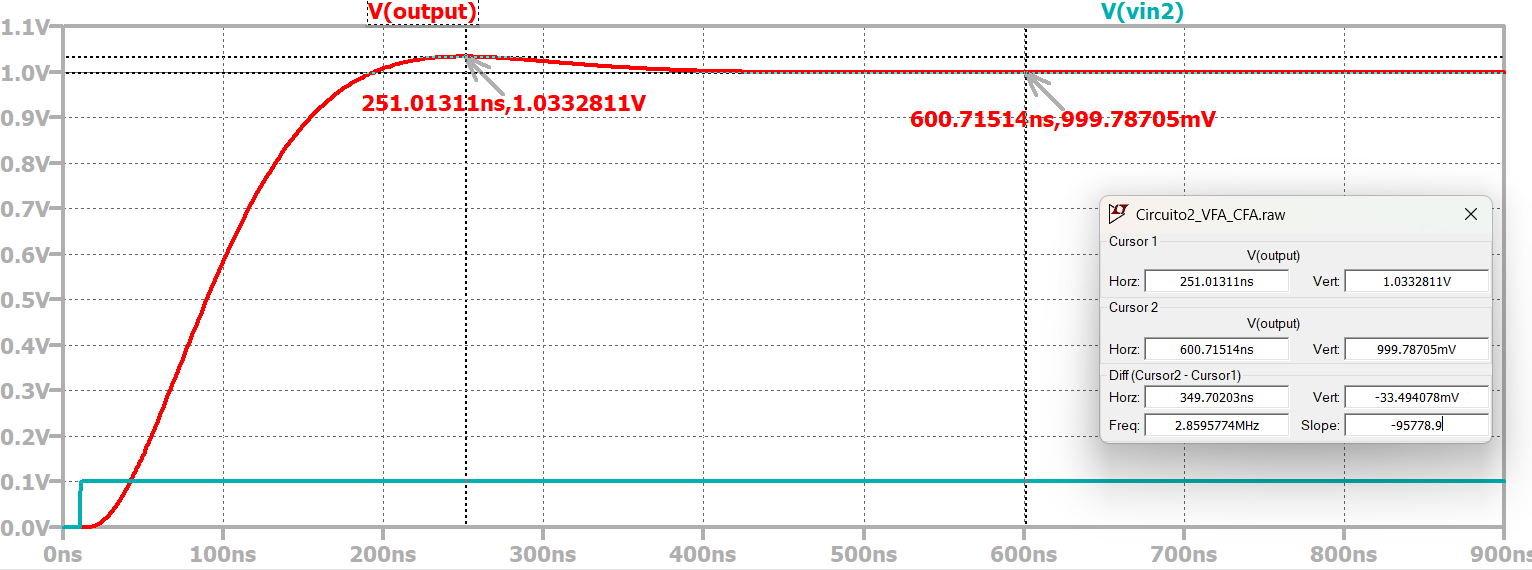
\includegraphics[width=0.95\linewidth,height=0.32\textheight,keepaspectratio]{Imagenes/c2_sim_escalon.png}
    \caption{Respuesta al escalón de $\SI{0,1}{V}$ (LTSpice): $V_{pico} = \SI{1,0333}{V}$ y $V_{est} = \SI{0,9998}{V}$.}
    \label{fig:rta_step_c2}
\end{figure}

\subsection{Comparación de resultados}
\label{sec:comparacion_c2}

\begin{table}[H]
\centering
\caption{Comparación entre teoría y simulación (VFA-CFA). Error $= (\text{teórico}-\text{LTSpice})/\text{LTSpice}$.}
\label{tab:final_c2}
\small
\setlength{\tabcolsep}{4pt}
\begin{tabularx}{\textwidth}{>{\raggedright\arraybackslash}X c c c c c}
\toprule
\textbf{Magnitud} & \textbf{Analítico} & \textbf{4 polos} & \textbf{LTSpice} & \textbf{Err. anal. [\%]} & \textbf{Err. 4p [\%]} \\
\midrule
Ancho de banda potencial $f_g$ [MHz] & 2,000 & --- & --- & --- & --- \\
Cruce de $T$ exacto $f_{Gc}$ [MHz] & 1,875 & 1,873 & 1,873 & $+0{,}1$ & $0{,}0$ \\
Margen de fase del lazo [$^\circ$] & 69,66 & 65,74 & 65,78 & $+5{,}9$ & $-0{,}1$ \\
Frecuencia de polos $f_p$ [MHz] & 3,181 & 3,165 & --- & --- & --- \\
Ancho de banda real $f_H$ [MHz] & 2,791 & 3,039 & 3,04 & $-8{,}1$ & $+0{,}1$ \\
Sobrepico \%OS [\%] & 1,62 & 3,36 & 3,35 & $-51{,}6$ & $+0{,}2$ \\
$M_\varphi$ desde el escalón [$^\circ$] & 69,66 & 66,88 & 66,89 & $+4{,}1$ & $0{,}0$ \\
\bottomrule
\end{tabularx}
\end{table}

\begin{table}[H]
\centering
\caption{Respuesta al escalón y margen de fase estimado, Caso 2.}
\label{tab:escalon_c2}
\begin{tabular}{lccc}
\toprule
\textbf{Magnitud} & \textbf{2 polos} & \textbf{4 polos} & \textbf{LTSpice} \\
\midrule
$V_{pico}$ [V] & 1,0162 & 1,0336 & 1,0333 \\
$V_{est}$ [V] & 1,0000 & 1,0000 & 0,9998 \\
$\mathrm{\char37}OS$ & 1,62 & 3,36 & 3,35 \\
$\zeta$ & 0,7953 & 0,7339 & 0,7341 \\
$M_\varphi$ estimado [$^\circ$] & 69,66 & 66,88 & 66,89 \\
\bottomrule
\end{tabular}
\end{table}

\subsection{Análisis y conclusión parcial}
\label{sec:concl_c2}

\begin{itemize}
    \item El diseño logra un ancho de banda potencial $f_g = K\,A_{vfi2}\,f_T = \SI{2}{MHz}$, unas $6{,}3$ veces el del compuesto VFA-VFA del Caso 1 ($\SI{316}{kHz}$), porque el CFA aporta ganancia local $A_{vfi2}=20$ sin perder ancho de banda. El cruce real de la ganancia de lazo ($f_{Gc} = \SI{1,87}{MHz}$ medido) queda por debajo de $f_g$ porque $f_g$ es el cruce asintótico; aun así es $\approx9$ veces el del Caso 1 ($\SI{206}{kHz}$).
    \item El ancho de banda real previsto ($\approx\SI{3}{MHz}$) supera a $f_g$, como en el Caso 1, porque con $Q_p\approx0{,}63$ a $0{,}68$ la respuesta es plana y la frecuencia de los polos ($f_p\approx\SI{3,2}{MHz}$) está por encima del cruce de $T$.
    \item El modelo de dos polos sobreestima el margen de fase en $\approx4^\circ$ ($69{,}7^\circ$ contra $65{,}7^\circ$) porque desprecia el atraso de fase de los polos del CFA. La tabla de sensibilidad muestra que el supuesto de $r_i$ modifica el margen de fase en menos de $3^\circ$.
    \item El valor de $A_{vfi2}$ se eligió por debajo de la cota de MPM ($25{,}3$), con la que el margen de fase del modelo de cuatro polos sería del orden de $60^\circ$ y habría pico en el módulo.
    \item La simulación coincide con el modelo de cuatro polos con errores menores al $0{,}2\,\mathrm{\char37}$ en $f_{Gc}$, margen de fase y sobrepico, lo que valida el modelo del CFA realimentado (\autoref{eq:Avf_CFA_ri}). El modelo de dos polos queda $\approx 4^\circ$ por encima en el margen de fase y predice la mitad del sobrepico.
    \item El margen de fase estimado a partir del escalón ($\ang{66,9}$) difiere en $\approx1^\circ$ del medido en el lazo ($\ang{65,8}$), diferencia esperable porque la relación entre sobrepico y margen de fase es exacta solo para segundo orden y aquí el sistema tiene cuatro polos.
    \item El ancho de banda real medido ($\approx\SI{3,04}{MHz}$) coincide con el modelo de cuatro polos y es $\approx8\,\mathrm{\char37}$ mayor que el del modelo de dos polos ($\SI{2,79}{MHz}$); ambos superan al potencial $f_g = \SI{2}{MHz}$ porque con $Q_p\approx0{,}68$ la respuesta es plana y $f_p>f_g$. No se observa pico en el módulo, como se esperaba para $Q_p<1/\sqrt2$ (apenas por debajo de MPM en el modelo simple).
    \item En conjunto, el compuesto VFA-CFA cumple los requerimientos: ganancia de $\SI{20}{dB}$, ancho de banda real de $\SI{3,04}{MHz}$ (frente a $\SI{345}{kHz}$ del compuesto VFA-VFA del Caso 1, casi $9$ veces mayor) y margen de fase de $\ang{65,8}$, equivalente al de MPM.
\end{itemize}

\section{Desarrollo: Caso 3, configuración VFA-CFA con red cero-polo}
\label{sec:desarrollo_c3}

\subsection{Diseño}
\label{sec:diseno_c3}

Al compuesto del Caso 2 se le agrega una red cero-polo a la salida del VFA (\autoref{eq:red_RC}, \autoref{sec:adelanto}): $C_x$ en paralelo con $R_x$ en serie entre la salida del LM324 y la entrada del CFA, y $R_y$ a tierra. Es la compensación con red a la salida del amplificador básico, donde el cero se ubica sobre el segundo polo del VFA ($D_x = z_x/p_2 \cong 1$, apunte Ec.~6.50 y 6.51) para cancelarlo, y el polo de la red queda una octava por encima, $f_{px} = 2f_{zx}$.

Con $\omega_{px}/\omega_{zx} = 1 + R_x/R_y = 2$ resulta $R_x = R_y$; adoptando $R_y = \SI{1}{k\ohm}$ queda $R_x = \SI{1}{k\ohm}$ y, para $f_{zx} = f_2$, $C_x = 1/(2\pi R_xf_2) = \SI{31,45}{pF}$. La atenuación de la red es $A_c(0) = R_y/(R_x+R_y) = 0{,}5$, por lo que se duplica la ganancia del CFA, $G_0' = G_0/A_c(0) = 40$, para conservar $T_0$ y $f_g$; entonces $R_1' = R_2/(G_0'-1) = \SI{21,03}{\ohm}$. El aumento de ganancia eleva $R_{eff}' = R_2 + r_iG_0' = \SI{1620}{\ohm}$ y baja el polo del CFA a $\SI{20,5}{MHz}$ (10 veces $f_g$); el CFA aislado conserva un margen de fase de $\ang{76,4}$.

\begin{table}[H]
\centering
\caption{Diseño VFA-CFA con red cero-polo: expresiones, cálculo y valores.}
\label{tab:parametros_vfa_cfa_red}
\footnotesize
\setlength{\tabcolsep}{4pt}
\begin{tabular}{>{\raggedright\arraybackslash}p{0.31\textwidth} >{\centering\arraybackslash}p{0.2\textwidth} >{\centering\arraybackslash}p{0.27\textwidth} >{\centering\arraybackslash}p{0.13\textwidth}}
\toprule
\textbf{Parámetro} & \textbf{Expresión} & \textbf{Cálculo} & \textbf{Valor} \\
\midrule
Ganancia global, $K$, $R_i$, $R_f$ & -- & igual que Caso 2 & \autoref{tab:parametros_vfa_cfa} \\
Resistencia a tierra de la red $R_y$ & elegida & -- & \SI{1}{k\ohm} \\
Resistencia serie de la red $R_x$ & $R_y(\omega_{px}/\omega_{zx}-1)$ & $1\text{ k}\Omega\cdot(2-1)$ & \SI{1}{k\ohm} \\
Capacitor de la red $C_x$ & $1/(2\pi R_xf_{zx})$ & $1/(2\pi\cdot 1\text{ k}\Omega\cdot 5{,}06\text{ MHz})$ & \SI{31,45}{pF} \\
Cero de la red $f_{zx}$ & $f_2$ & -- & \SI{5,06}{MHz} \\
Polo de la red $f_{px}$ & $1/(2\pi C_x(R_x\parallel R_y))$ & $2f_{zx}$ & \SI{10,12}{MHz} \\
Atenuación de la red $A_c(0)$ & $R_y/(R_x+R_y)$ & $1/2$ & \num{0,5} \\
Ganancia del CFA retocada $G_0'$ & $G_0/A_c(0)$ & $20/0{,}5$ & \SI{40}{V/V} \\
Resistencia local a tierra $R_1'$ & $R_2/(G_0'-1)$ & $820/39$ & \SI{21,03}{\ohm} \\
Resistencia efectiva $R_{eff}'$ & $R_2+r_iG_0'$ & $820+20\cdot 40$ & \SI{1620}{\ohm} \\
Ganancia de lazo en continua $T_0$ & $K\,A_{d0}\,A_c(0)\,G_0'$ & $0{,}1\cdot10^5\cdot0{,}5\cdot40$ & \num{200000} (\SI{106}{dB}) \\
Separación de polos $D_p$ & $f_{px}/f_1$ & $10{,}12\text{ MHz}/10\text{ Hz}$ & \num{1012000} \\
\bottomrule
\end{tabular}
\end{table}

\subsection{Resultados analíticos}
\label{sec:analitico_c3}

Con el cero cancelando el segundo polo del VFA, el producto $A_1A_c$ queda con los polos $f_1$ y $f_{px}$, y la ganancia de lazo es $T(s) \cong T_0/[(1+s/\omega_1)(1+s/\omega_{px})]$ con el mismo $T_0$ y $f_g$ que en el Caso 2. Como $D_p$ se duplicó, $Q_p^2 = f_g/f_{px} = 0{,}198$ es la mitad que en el Caso 2 y los polos de lazo cerrado resultan reales y distintos (respuesta sobreamortiguada, $\zeta>1$). La \autoref{tab:analitica_c3} reúne los resultados; el margen de fase del modelo simple se verificó también con la fórmula del apunte.

\begin{table}[H]
\centering
\caption{Resultados analíticos (modelo de dos polos), Caso 3.}
\label{tab:analitica_c3}
\small
\setlength{\tabcolsep}{4pt}
\begin{tabular}{>{\raggedright\arraybackslash}p{0.37\textwidth} >{\centering\arraybackslash}p{0.31\textwidth} >{\centering\arraybackslash}p{0.2\textwidth}}
\toprule
\textbf{Magnitud} & \textbf{Expresión} & \textbf{Valor} \\
\midrule
Ancho de banda potencial $f_g$ & $K\,A_c(0)\,G_0'\,f_T$ & \SI{2,000}{MHz} \\
Cruce exacto de $T$, $f_{Gc}$ & $|T(jf)|=1$ & \SI{1,963}{MHz} \\
$\Omega_G = f_{Gc}/f_p$ & -- & \num{0,4364} \\
Margen de fase $M_\varphi$ & \autoref{eq:Mphi_2polos} & \ang{79,02} \\
Frecuencia de los polos $f_p$ & $\sqrt{\omega_1\omega_{px}(1+T_0)}/2\pi$ & \SI{4,499}{MHz} \\
Factor de calidad $Q_p$ & $\omega_p/(\omega_1+\omega_{px})$ & \num{0,445} \\
Amortiguamiento $\zeta$ & $1/(2Q_p)$ & \num{1,125} \\
Polos de lazo cerrado & $s_{1,2}$ & $\approx -2{,}74$ y $-7{,}36$ MHz (reales) \\
Ancho de banda real $f_H$ ($-3$ dB) & $f_p\sqrt{a+\sqrt{a^2+1}}$ & \SI{2,455}{MHz} \\
\bottomrule
\end{tabular}
\end{table}

El modelo de cuatro polos incluye el CFA realimentado con $G_0'$ y $R_{eff}'$ (\autoref{tab:modelos_c3}). Los polos del CFA agregan atraso de fase, por lo que el margen de fase baja a $\ang{73,6}$ y el par dominante pasa a ser complejo con $Q_p = 0{,}503$, prácticamente sin pico.

\begin{table}[H]
\centering
\caption{Resultados numéricos: modelo de 2 polos y de 4 polos, Caso 3.}
\label{tab:modelos_c3}
\begin{tabular}{lcc}
\toprule
\textbf{Magnitud} & \textbf{2 polos} & \textbf{4 polos} \\
\midrule
Frecuencia crítica $f_{Gc}$ [MHz] & 1,963 & 1,958 \\
Margen de fase [$^\circ$] & 79,02 & 73,58 \\
Margen de ganancia [dB] & $\infty$ & 22,0 \\
Ancho de banda real ($-3$ dB) [MHz] & 2,455 & 2,826 \\
Frecuencia de los polos $f_p$ [MHz] & 4,499 & 4,391 \\
Factor de calidad $Q_p$ & 0,445 & 0,503 \\
Polos dominantes [MHz] & $-2{,}744$ (real) & $-4{,}368 \pm j\,0{,}453$ \\
\bottomrule
\end{tabular}
\end{table}

\begin{figure}[H]
    \centering
    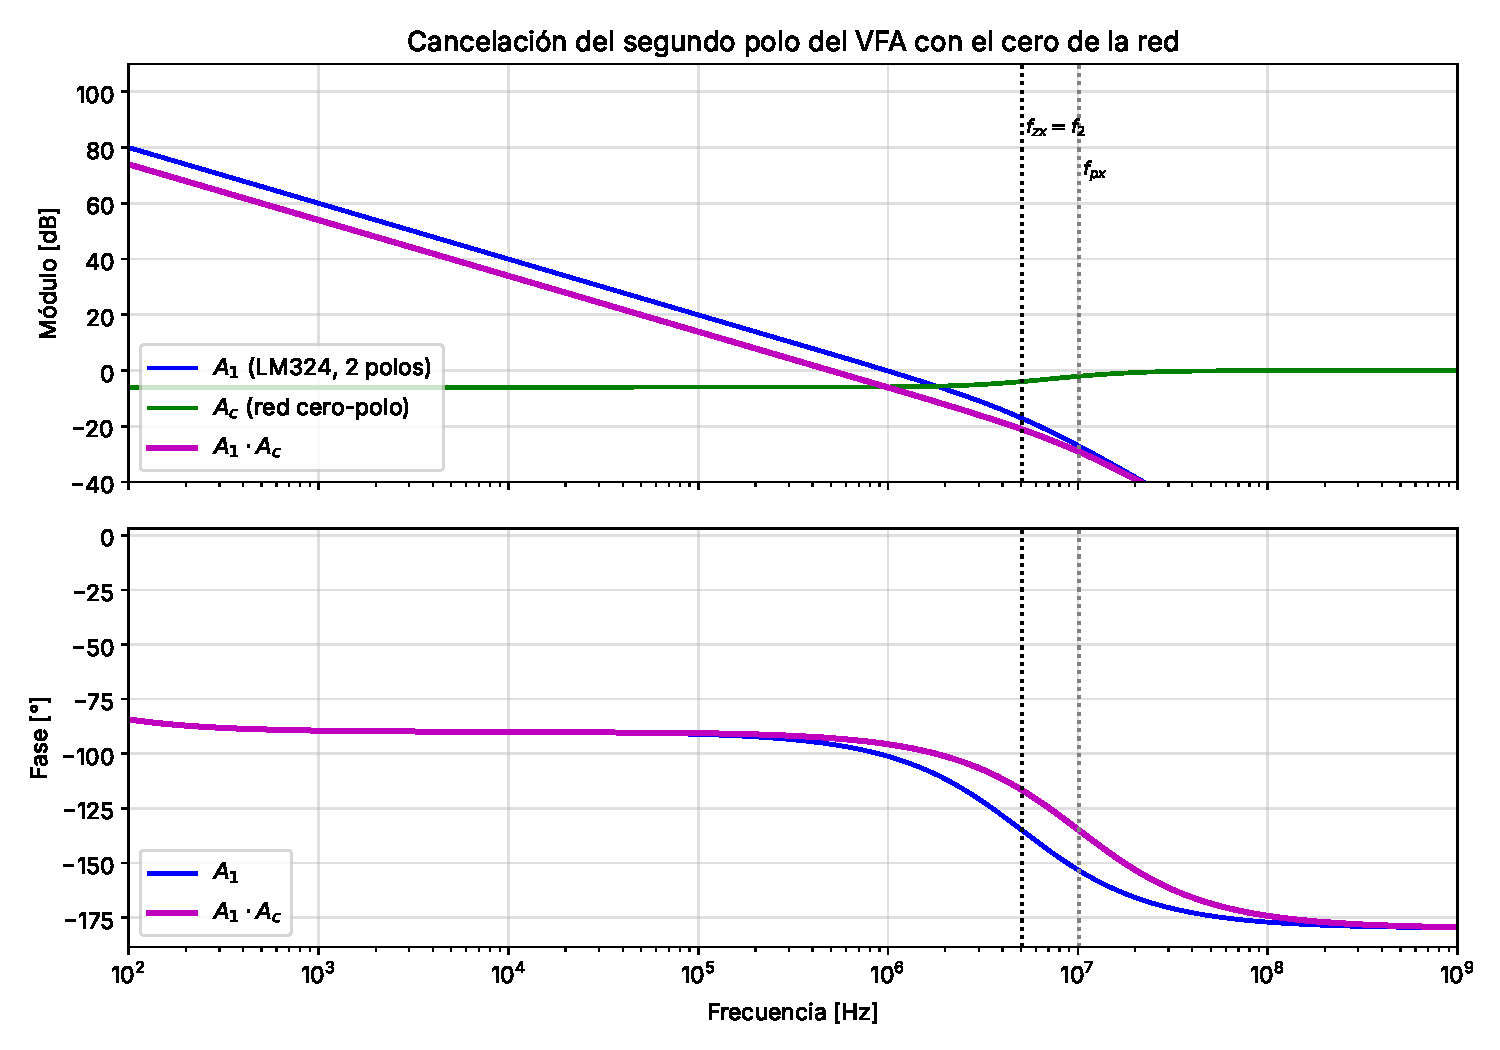
\includegraphics[width=0.85\linewidth,height=0.28\textheight,keepaspectratio]{Imagenes/c3_cancelacion_polo.pdf}
    \caption{Cancelación del segundo polo del VFA con el cero de la red: módulo y fase de $A_1$, $A_c$ y $A_1A_c$.}
    \label{fig:cancelacion_c3}
\end{figure}

\begin{figure}[H]
    \centering
    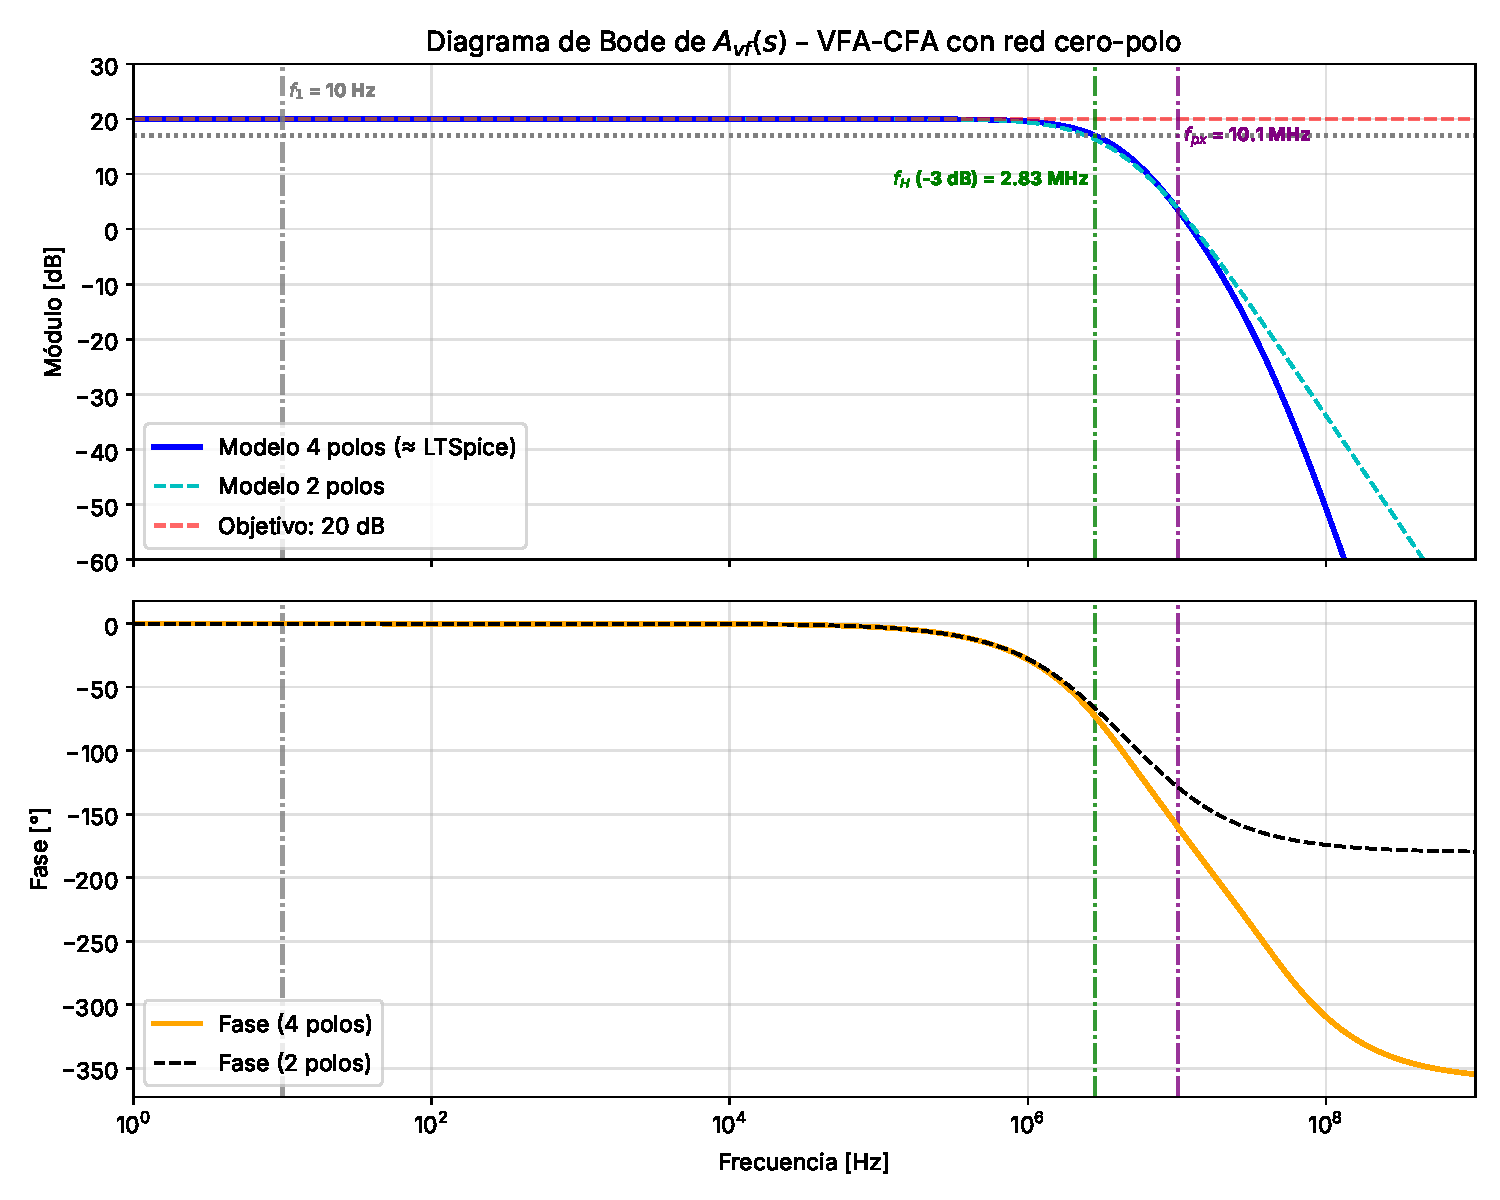
\includegraphics[width=0.85\linewidth,height=0.28\textheight,keepaspectratio]{Imagenes/c3_bode_lazo_cerrado.pdf}
    \caption{Diagrama de Bode a lazo cerrado (modelos de 2 y 4 polos), Caso 3.}
    \label{fig:bode_lc_c3}
\end{figure}

\begin{figure}[H]
    \centering
    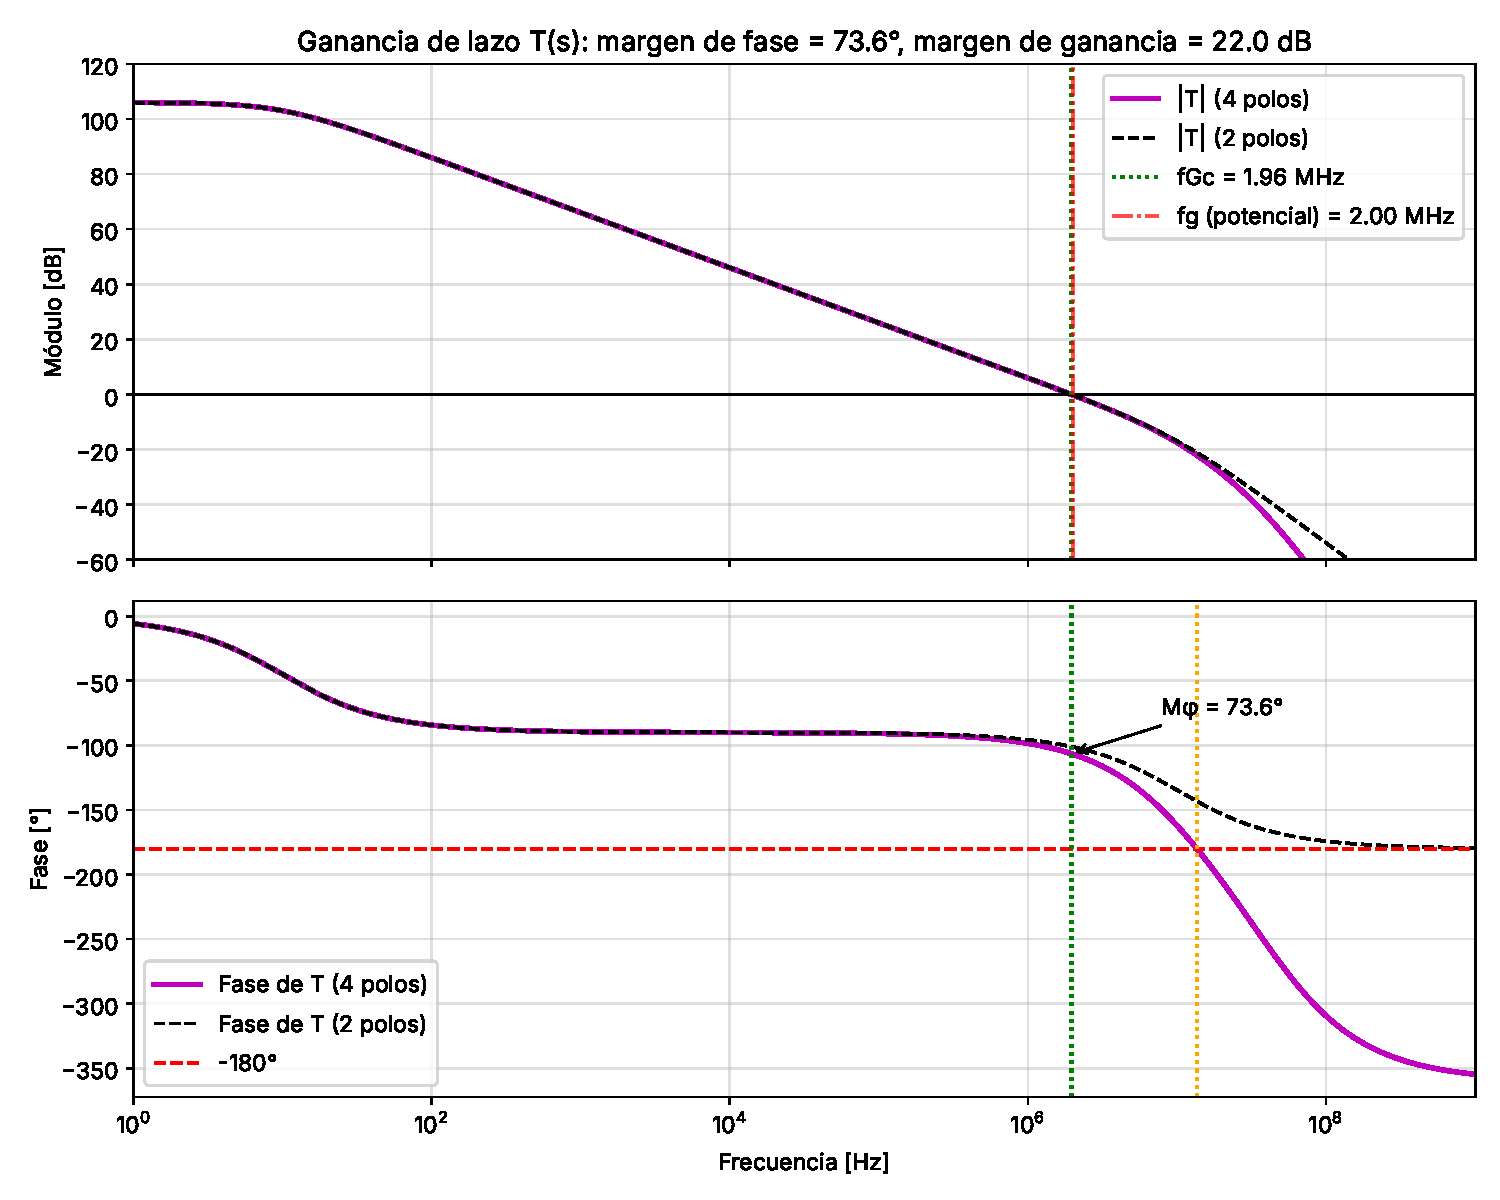
\includegraphics[width=0.85\linewidth,height=0.28\textheight,keepaspectratio]{Imagenes/c3_bode_ganancia_lazo.pdf}
    \caption{Diagrama de Bode de la ganancia de lazo, Caso 3: frecuencia crítica y margen de fase.}
    \label{fig:bode_lazo_c3}
\end{figure}

\paragraph{Comparación con el Caso 2.} La \autoref{tab:comp_teo_c3} y la \autoref{fig:comparacion_c3} muestran la mejora: con el mismo $T_0$ y $f_g$, el margen de fase sube $\ang{7,8}$ y el sobrepico desaparece, a costa de un ancho de banda real $\approx7\,\mathrm{\char37}$ menor (respuesta más amortiguada).

\begin{table}[H]
\centering
\caption{Caso 2 contra Caso 3 (teoría, modelo de 4 polos).}
\label{tab:comp_teo_c3}
\begin{tabular}{lcc}
\toprule
\textbf{Magnitud} & \textbf{Caso 2 (sin red)} & \textbf{Caso 3 (con red)} \\
\midrule
Frecuencia crítica $f_{Gc}$ [MHz] & 1,873 & 1,958 \\
Margen de fase [$^\circ$] & 65,74 & 73,58 \\
Margen de ganancia [dB] & 23,2 & 22,0 \\
Ancho de banda real ($-3$ dB) [MHz] & 3,039 & 2,826 \\
Factor de calidad $Q_p$ & 0,681 & 0,503 \\
Sobrepico \%OS (escalón) [\%] & 3,36 & sin sobrepico \\
\bottomrule
\end{tabular}
\end{table}

\begin{figure}[H]
    \centering
    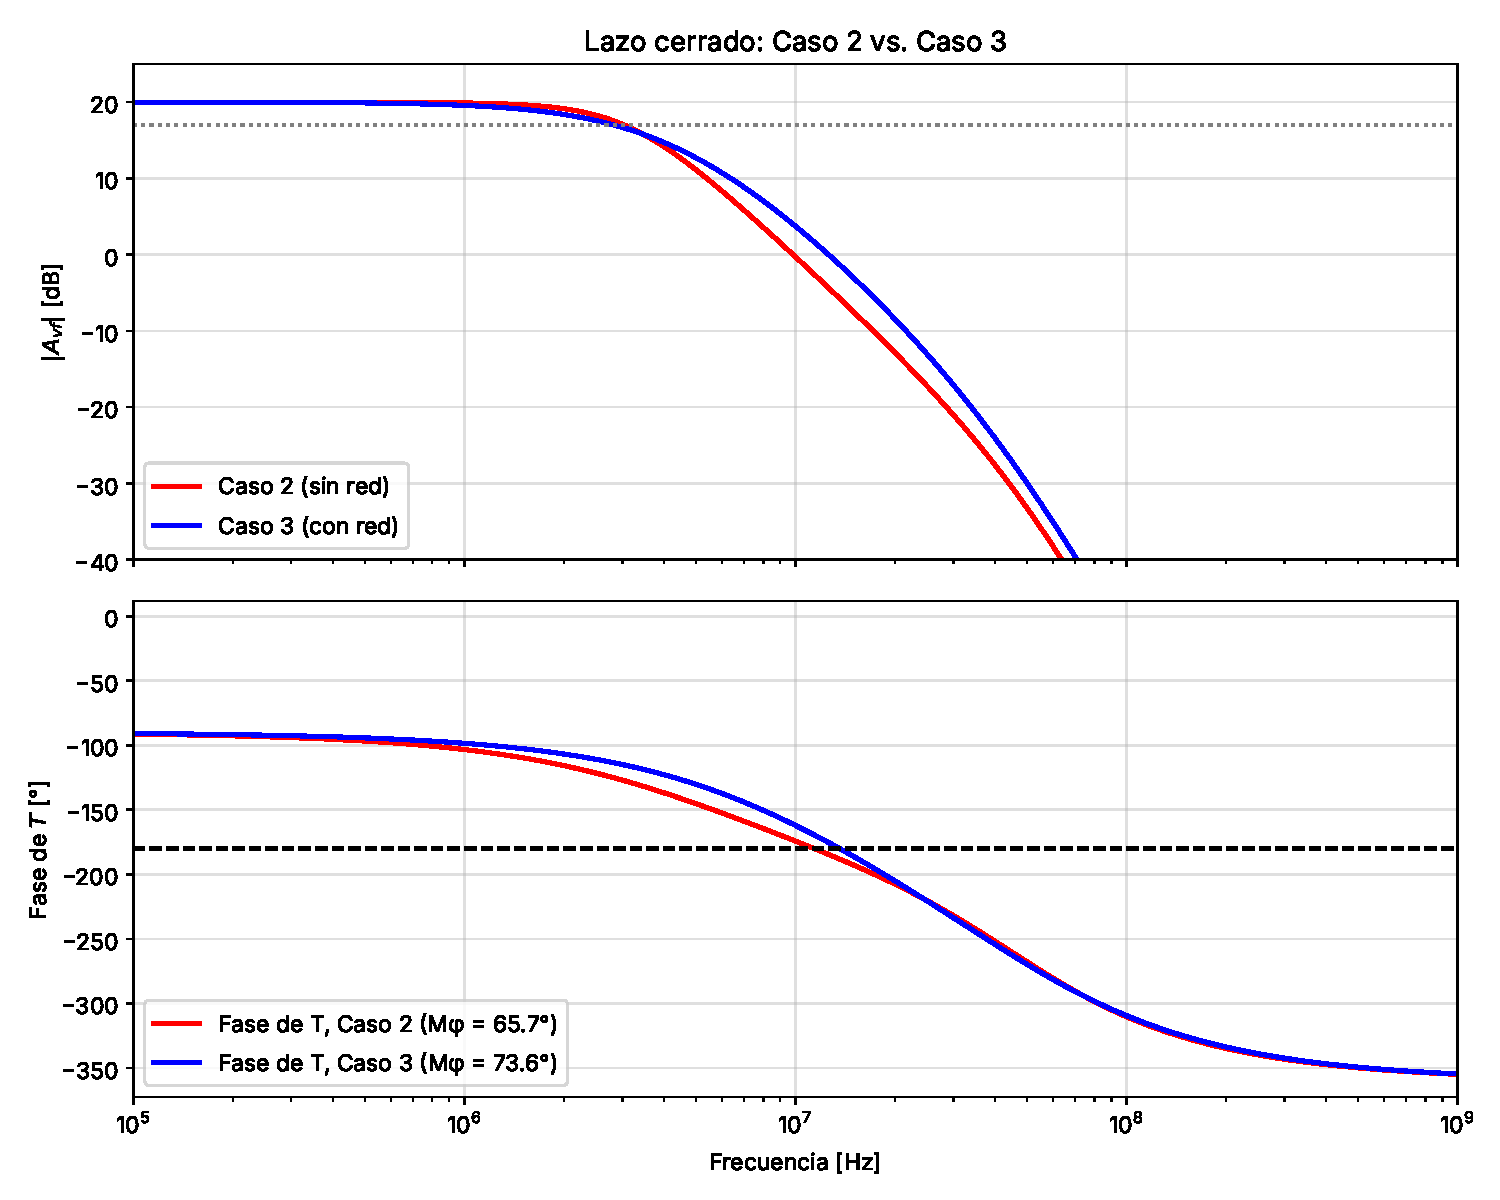
\includegraphics[width=0.85\linewidth,height=0.28\textheight,keepaspectratio]{Imagenes/c3_comparacion_caso2.pdf}
    \caption{Lazo cerrado y fase de $T$: Caso 2 contra Caso 3.}
    \label{fig:comparacion_c3}
\end{figure}

\paragraph{Sensibilidad al valor de $r_i$.} Con $r_i$ entre $0$ y $\SI{50}{\ohm}$ el margen de fase del modelo de cuatro polos varía entre $\ang{76,2}$ y $\ang{69,7}$ (\autoref{tab:ri_c3}); en todos los casos supera al del Caso 2 con el mismo $r_i$.

\begin{table}[H]
\centering
\caption{Sensibilidad al valor de $r_i$ (modelo de 4 polos), Caso 3.}
\label{tab:ri_c3}
\begin{tabular}{cccccc}
\toprule
$r_i$ [$\Omega$] & $R_{eff}'$ [$\Omega$] & $f_{Gc}$ [MHz] & $M_\varphi$ [$^\circ$] & $M_G$ [dB] & BW [MHz] \\
\midrule
0 & 820 & 1,963 & 76,2 & 26,3 & 2,637 \\
10 & 1220 & 1,961 & 74,9 & 23,7 & 2,731 \\
20 & 1620 & 1,958 & 73,6 & 22,0 & 2,826 \\
30 & 2020 & 1,954 & 72,3 & 20,9 & 2,920 \\
50 & 2820 & 1,943 & 69,7 & 19,3 & 3,093 \\
\bottomrule
\end{tabular}
\end{table}

\paragraph{Respuesta al escalón teórica.} La \autoref{fig:escalon_teorico_c3} muestra la respuesta a un escalón de $\SI{0,1}{V}$ (salida de $\SI{1}{V}$) del Caso 3 y la \autoref{fig:escalon_comparacion_c3} la compara con la del Caso 2. En el Caso 3 no hay sobrepico ($\mathrm{\char37}OS<0{,}05\,\mathrm{\char37}$), por lo que la fórmula de la \autoref{eq:zeta} no es aplicable: la ausencia de sobrepico indica $\zeta \gtrsim 0{,}9$, es decir $M_\varphi \gtrsim 73^\circ$ por la \autoref{eq:MF_exacta}, y la mejora se constata comparando con el sobrepico del Caso 2 ($3{,}36\,\mathrm{\char37}$).

\begin{figure}[H]
    \centering
    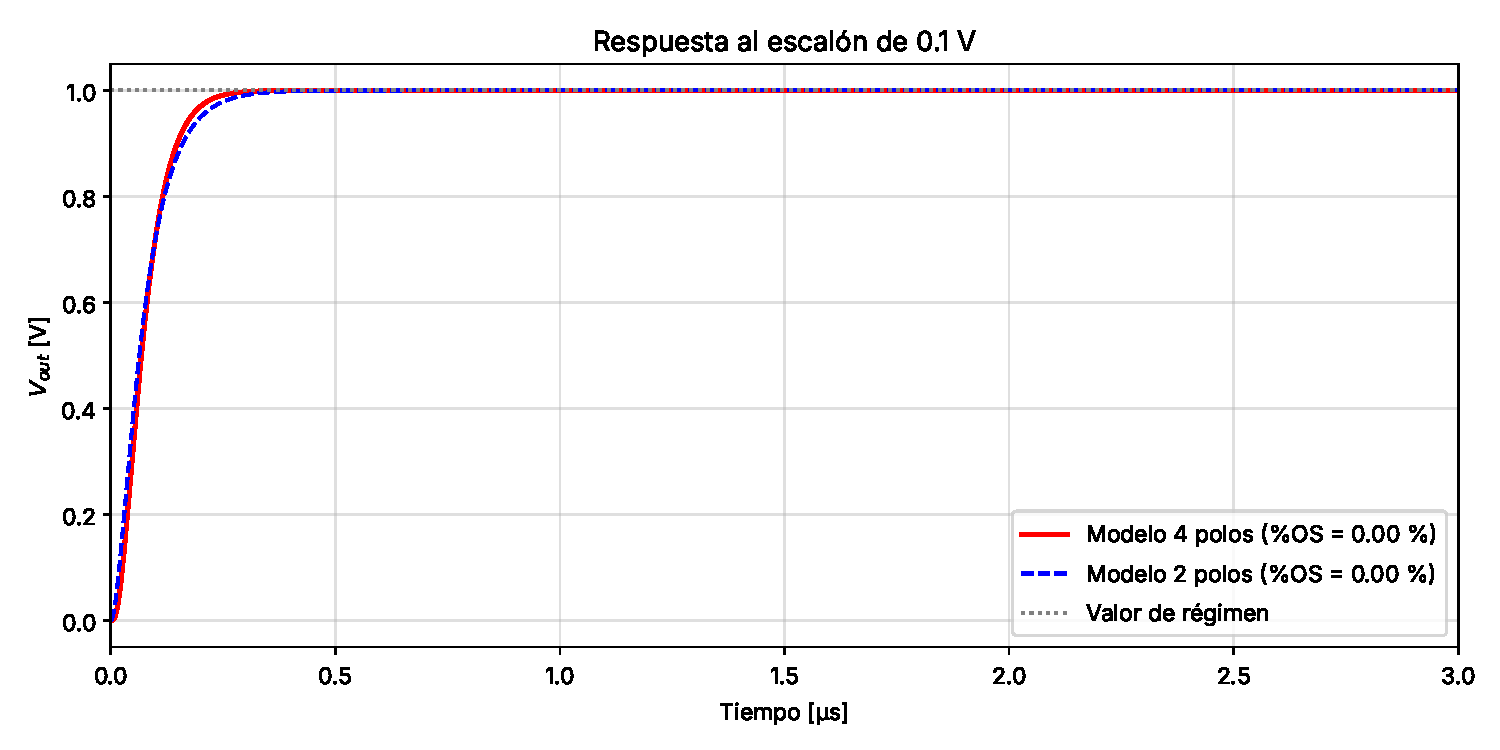
\includegraphics[width=0.85\linewidth,height=0.28\textheight,keepaspectratio]{Imagenes/c3_escalon_teorico.pdf}
    \caption{Respuesta al escalón teórica (2 y 4 polos), Caso 3.}
    \label{fig:escalon_teorico_c3}
\end{figure}

\begin{figure}[H]
    \centering
    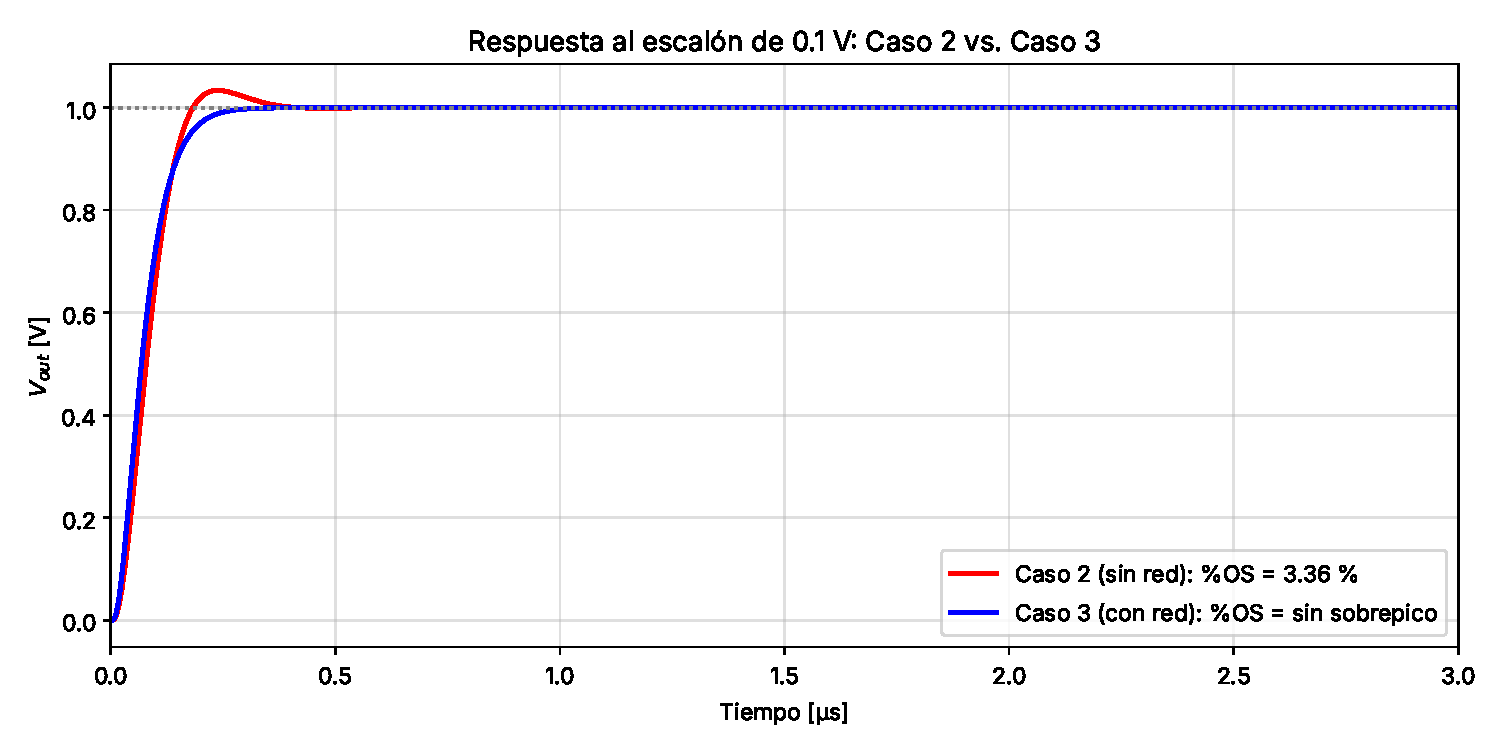
\includegraphics[width=0.85\linewidth,height=0.28\textheight,keepaspectratio]{Imagenes/c3_escalon_comparacion.pdf}
    \caption{Respuesta al escalón teórica: Caso 2 contra Caso 3.}
    \label{fig:escalon_comparacion_c3}
\end{figure}

\subsection{Simulación}
\label{sec:simulacion_c3}

Se simularon en LTSpice los mismos tres circuitos del Caso 2 (\autoref{fig:circuito_VFA_CFA_red}), agregando la red $R_x\parallel C_x$, $R_y$ entre la salida del LM324 y la entrada no inversora del LM6181, con $R_x=R_y=\SI{1}{k\ohm}$, $C_x=\SI{31,45}{pF}$ y $R_1'=\SI{21,03}{\ohm}$ ($R_2=\SI{820}{\ohm}$, $R_i=\SI{1}{k\ohm}$, $R_f=\SI{9}{k\ohm}$).

\begin{figure}[H]
    \centering
    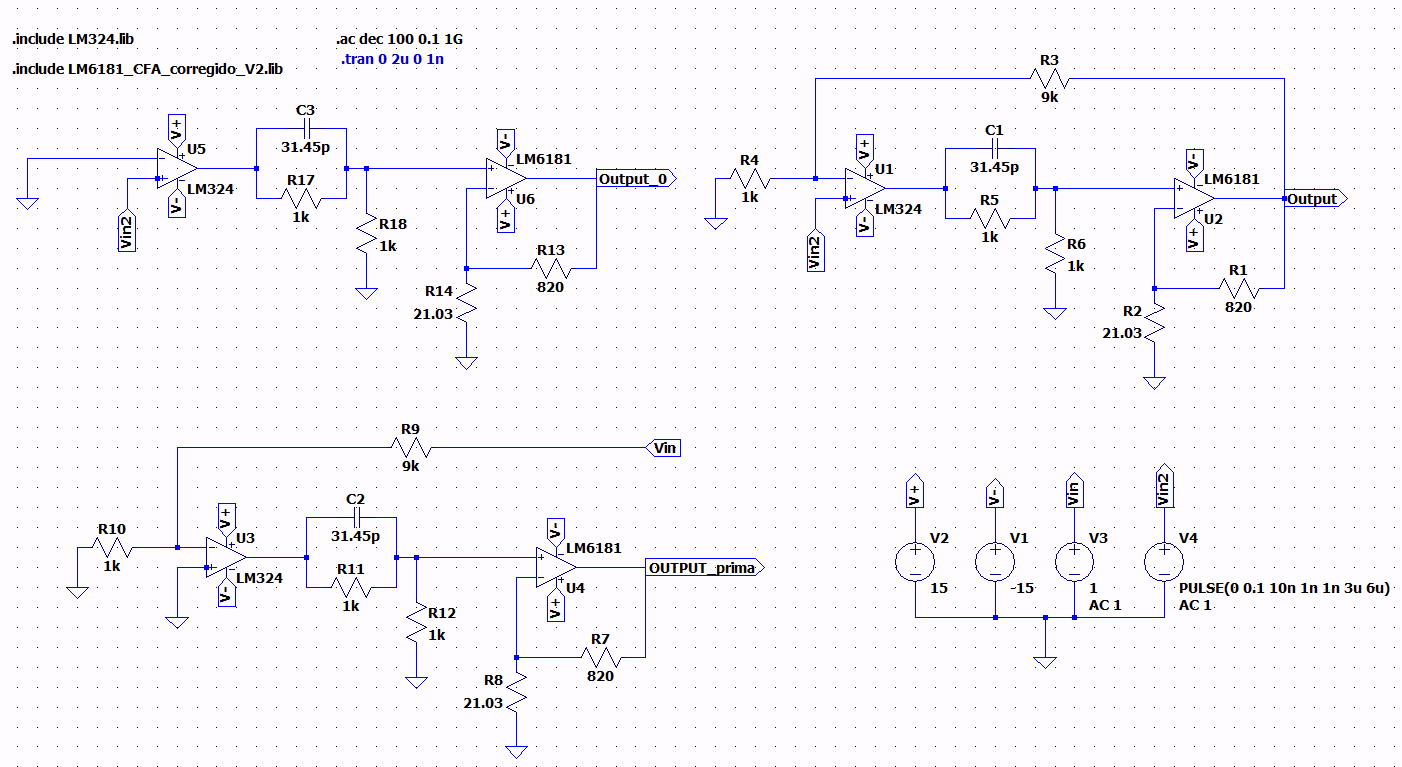
\includegraphics[width=1.0\linewidth,height=0.28\textheight,keepaspectratio]{Imagenes/c3_sim_circuitos.png}
    \caption{Esquemático VFA-CFA con red cero-polo en LTSpice: lazo abierto (arriba a la izquierda), lazo cerrado (arriba a la derecha) y ganancia de lazo (abajo).}
    \label{fig:circuito_VFA_CFA_red}
\end{figure}

\subsubsection{Respuesta en frecuencia a lazo abierto}
La \autoref{fig:rta_frec_open_loop_c3} muestra una ganancia en banda media de $A_{d0}A_c(0)G_0' = 100\text{ dB} + 26\text{ dB} = 126\text{ dB}$ (igual que el Caso 2), con el polo dominante en $f_1=\SI{10}{Hz}$. La fase se mantiene cerca de $-90^\circ$ hasta varios MHz: la red cancela el cambio de pendiente que el segundo polo del VFA produciría en $f_2=\SI{5,06}{MHz}$, y el atraso de fase aparece recién con el polo de la red y los del CFA.

\begin{figure}[H]
    \centering
    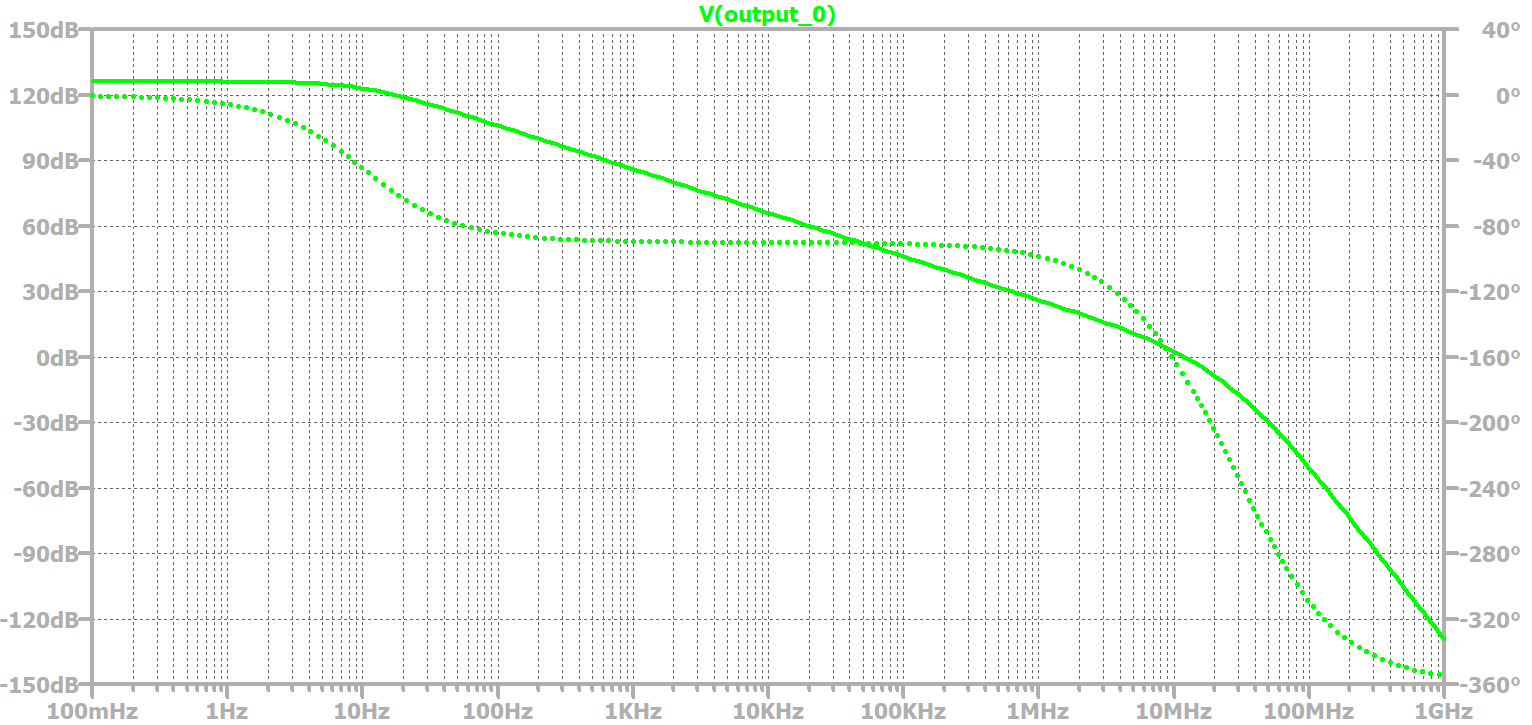
\includegraphics[width=0.85\linewidth,height=0.28\textheight,keepaspectratio]{Imagenes/c3_sim_lazo_abierto.png}
    \caption{Respuesta en frecuencia a \textbf{lazo abierto} del compuesto con red cero-polo (módulo y fase).}
    \label{fig:rta_frec_open_loop_c3}
\end{figure}

\subsubsection{Respuesta en frecuencia de la ganancia de lazo}
En la \autoref{fig:rta_frec_loop_c3} se midió sobre la curva de $-T$ (\texttt{V(output\_prima)}) el cruce por \SI{0}{dB} en $f_{Gc} = \SI{1,957}{MHz}$, donde la fase es $M_\varphi = \ang{73,62}$ (el modelo de cuatro polos predice \SI{1,958}{MHz} y \ang{73,58}). La ganancia de lazo en continua es de \SI{106}{dB}, igual que en el Caso 2.

\begin{figure}[H]
    \centering
    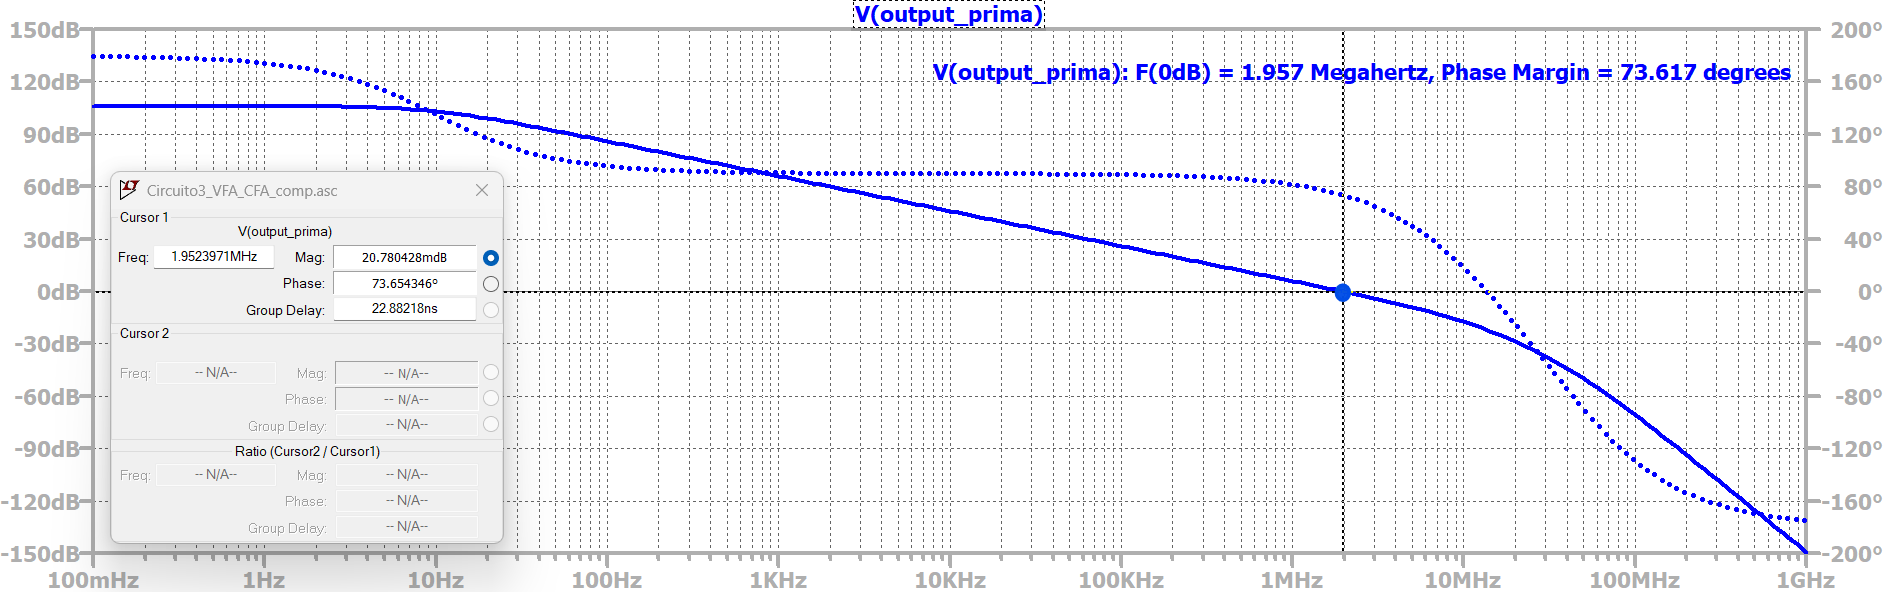
\includegraphics[width=0.85\linewidth,height=0.28\textheight,keepaspectratio]{Imagenes/c3_sim_lazo_T.png}
    \caption{Respuesta en frecuencia de la \textbf{ganancia de lazo} ($-T$): $f_{Gc} = \SI{1,957}{MHz}$ y $M_\varphi = \ang{73,62}$.}
    \label{fig:rta_frec_loop_c3}
\end{figure}

\subsubsection{Respuesta en frecuencia a lazo cerrado}
La \autoref{fig:rta_frec_close_loop_c3} confirma la ganancia en banda media de $\SI{20}{dB}$ ($\SI{19,99996}{dB}$ a $\SI{30}{Hz}$), sin sobrepico. Con el cursor a $\SI{17}{dB}$ se obtuvo $\SI{17,004}{dB}$ a $\SI{2,815}{MHz}$ ($-3{,}00$ dB respecto de banda media); interpolando al punto de $-3{,}01$ dB resulta un ancho de banda real $f_H \approx \SI{2,82}{MHz}$ (el modelo de cuatro polos predice $\SI{2,826}{MHz}$).

\begin{figure}[H]
    \centering
    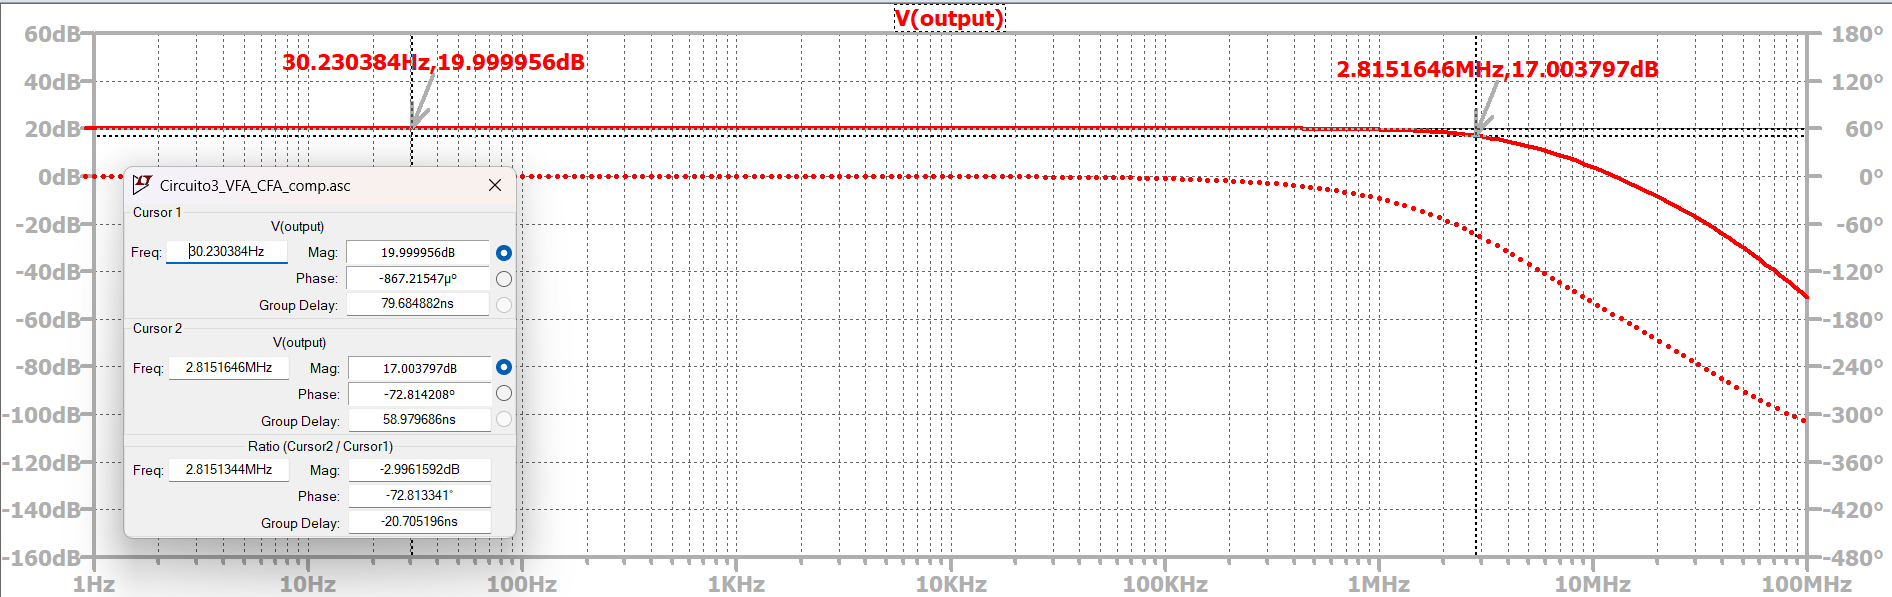
\includegraphics[width=0.85\linewidth,height=0.28\textheight,keepaspectratio]{Imagenes/c3_sim_lazo_cerrado.png}
    \caption{Respuesta en frecuencia a \textbf{lazo cerrado}.}
    \label{fig:rta_frec_close_loop_c3}
\end{figure}

\subsubsection{Respuesta al escalón}
Se aplicó un escalón de $\SI{0,1}{V}$ (salida de $\SI{1}{V}$) con flancos de $\SI{1}{ns}$. La salida (\autoref{fig:rta_step_c3}) crece de forma monótona hasta $\SI{1}{V}$ y se asienta en $\approx\SI{300}{ns}$, \emph{sin sobrepico visible}, como predice el modelo. El Caso 2, con el mismo escalón, tenía un sobrepico de $3{,}35\,\mathrm{\char37}$ (\autoref{fig:rta_step_c2}). Como no hay sobrepico no puede estimarse $\zeta$ ni el margen de fase con las \autoref{eq:zeta} y \autoref{eq:MF_exacta}; solo se concluye que $\zeta \gtrsim 0{,}9$ y $M_\varphi \gtrsim 73^\circ$, consistente con los $\ang{73,6}$ medidos en el lazo.

\begin{figure}[H]
    \centering
    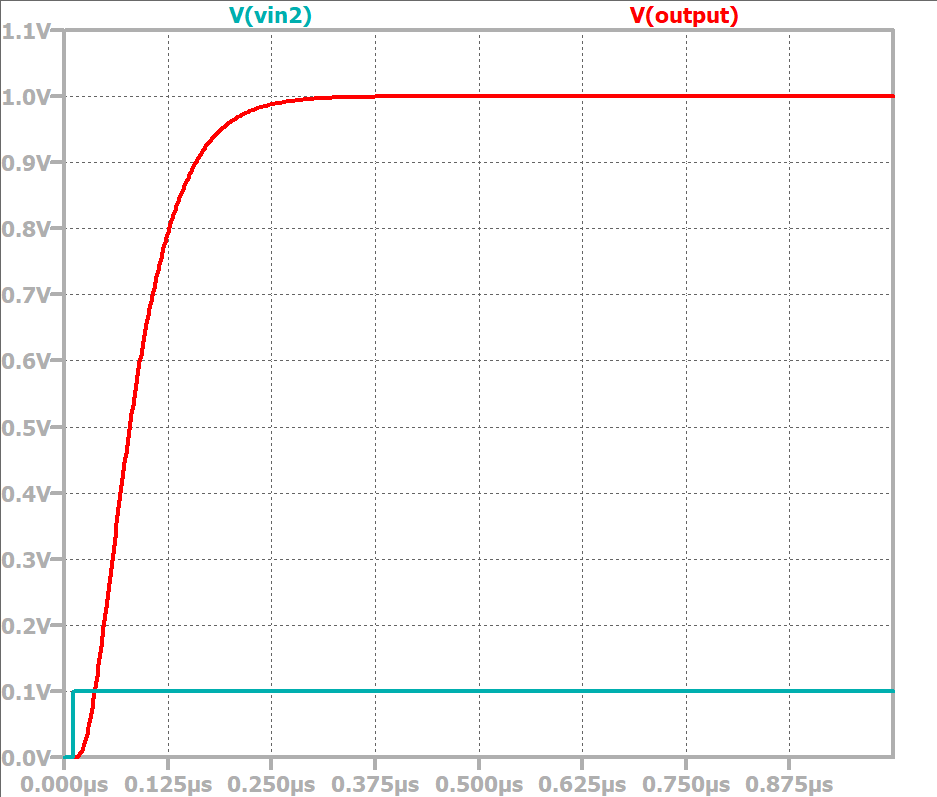
\includegraphics[width=0.85\linewidth,height=0.28\textheight,keepaspectratio]{Imagenes/c3_sim_escalon.png}
    \caption{Respuesta al escalón de $\SI{0,1}{V}$ (LTSpice), Caso 3: sin sobrepico.}
    \label{fig:rta_step_c3}
\end{figure}

\subsection{Comparación de resultados}
\label{sec:comparacion_c3}

La \autoref{tab:final_c3} compara los valores analíticos (dos polos), el modelo de cuatro polos y las mediciones de LTSpice, y la \autoref{tab:comp_sim_c3} contrasta los dos compuestos con medidas de simulación.

\begin{table}[H]
\centering
\caption{Comparación entre teoría y simulación (VFA-CFA con red). Error $= (\text{teórico}-\text{LTSpice})/\text{LTSpice}$.}
\label{tab:final_c3}
\small
\setlength{\tabcolsep}{4pt}
\setlength{\tabcolsep}{4pt}
\begin{tabularx}{\textwidth}{>{\raggedright\arraybackslash}X c c c c c}
\toprule
\textbf{Magnitud} & \textbf{Analítico} & \textbf{4 polos} & \textbf{LTSpice} & \textbf{Err. anal. [\%]} & \textbf{Err. 4p [\%]} \\
\midrule
Ancho de banda potencial $f_g$ [MHz] & 2,000 & -- & -- & -- & -- \\
Cruce de $T$ exacto $f_{Gc}$ [MHz] & 1,963 & 1,958 & 1,957 & $+0{,}3$ & $0{,}0$ \\
Margen de fase del lazo [$^\circ$] & 79,02 & 73,58 & 73,62 & $+7{,}3$ & $0{,}0$ \\
Frecuencia de polos $f_p$ [MHz] & 4,499 & 4,391 & -- & -- & -- \\
Ancho de banda real $f_H$ [MHz] & 2,455 & 2,826 & 2,82 & $-13{,}0$ & $+0{,}1$ \\
Sobrepico \%OS [\%] & 0 & 0 & sin sobrepico & -- & -- \\
\bottomrule
\end{tabularx}
\end{table}

\begin{table}[H]
\centering
\caption{Caso 2 contra Caso 3: modelo de 4 polos y simulación en LTSpice.}
\label{tab:comp_sim_c3}
\small
\setlength{\tabcolsep}{4pt}
\begin{tabular}{lcccc}
\toprule
 & \multicolumn{2}{c}{\textbf{Caso 2 (sin red)}} & \multicolumn{2}{c}{\textbf{Caso 3 (con red)}} \\
\textbf{Magnitud} & 4 polos & LTSpice & 4 polos & LTSpice \\
\midrule
Frecuencia crítica $f_{Gc}$ [MHz] & 1,873 & 1,873 & 1,958 & 1,957 \\
Margen de fase del lazo [$^\circ$] & 65,74 & 65,78 & 73,58 & 73,62 \\
Ancho de banda real [MHz] & 3,039 & 3,04 & 2,826 & 2,82 \\
Sobrepico \%OS [\%] & 3,36 & 3,35 & 0 & sin sobrepico \\
\bottomrule
\end{tabular}
\end{table}

\subsection{Análisis y conclusión parcial}
\label{sec:concl_c3}

\begin{itemize}
    \item La red cero-polo cancela el segundo polo del LM324 y desplaza el nuevo segundo polo de $\SI{5,06}{MHz}$ a $\SI{10,12}{MHz}$. Con $T_0$ y $f_g$ iguales a los del Caso 2, el margen de fase medido mejora de $\ang{65,78}$ a $\ang{73,62}$ (mejora de $\ang{7,8}$, igual a la prevista por el modelo) y el sobrepico del escalón pasa de $3{,}35\,\mathrm{\char37}$ a nulo.
    \item La simulación coincide con el modelo de cuatro polos con errores menores al $0{,}3\,\mathrm{\char37}$ en $f_{Gc}$, margen de fase y ancho de banda, lo que valida el modelo del compuesto con la red. El modelo de dos polos sobreestima el margen de fase en $\approx5^\circ$ ($79{,}0^\circ$ contra $73{,}6^\circ$), porque desprecia el atraso de fase de los polos del CFA, y subestima el ancho de banda ($13\,\mathrm{\char37}$).
    \item La mejora tiene un costo: la respuesta queda más amortiguada y el ancho de banda real baja de $\SI{3,04}{MHz}$ a $\SI{2,82}{MHz}$ ($\approx7\,\mathrm{\char37}$), y se necesita duplicar la ganancia del CFA, lo que aumenta $R_{eff}'$ y baja su polo de $\SI{27,2}{MHz}$ a $\SI{20,5}{MHz}$ (sigue siendo $10$ veces $f_g$). Aun así el ancho de banda es unas $8$ veces el del compuesto VFA-VFA del Caso 1 ($\SI{345}{kHz}$).
    \item Como no hay sobrepico en el escalón, el margen de fase no puede estimarse por ese método; solo se acota ($M_\varphi \gtrsim 73^\circ$), consistente con el valor medido en el lazo.
    \item La cancelación es exacta solo en el modelo: en el circuito real depende de las tolerancias de $R_x$ y $C_x$ y de la impedancia de salida del VFA, por lo que el cero puede correrse y la mejora real ser menor.
\end{itemize}

\newpage
\section{Conclusiones}
\label{sec:conclusiones}

En este trabajo se diseñaron, calcularon y simularon tres amplificadores compuestos de $\SI{20}{dB}$ de ganancia con el objetivo de alcanzar una respuesta de máxima planicidad de módulo (MPM): VFA-VFA (Caso 1), VFA-CFA (Caso 2) y VFA-CFA con red de compensación cero-polo (Caso 3). La \autoref{tab:resumen_final} resume las mediciones de LTSpice de los tres casos.

\begin{table}[H]
\centering
\caption{Resumen de resultados medidos en LTSpice de los tres casos.}
\label{tab:resumen_final}
\small
\setlength{\tabcolsep}{4pt}
\begin{tabular}{lcccc}
\toprule
\textbf{Magnitud} & \textbf{Caso 1} & \textbf{Caso 2} & \textbf{Caso 3} & \textbf{MPM} \\
\midrule
Cruce de la ganancia de lazo $f_{Gc}$ & \SI{206}{kHz} & \SI{1,87}{MHz} & \SI{1,96}{MHz} & --- \\
Margen de fase del lazo $M_\varphi$ & \ang{62,5} & \ang{65,8} & \ang{73,6} & \ang{65,5} \\
Ancho de banda real $f_H$ ($-3$ dB) & \SI{345}{kHz} & \SI{3,04}{MHz} & \SI{2,82}{MHz} & --- \\
Sobrepico del escalón & $5{,}83\,\mathrm{\char37}$ & $3{,}35\,\mathrm{\char37}$ & sin sobrepico & --- \\
\bottomrule
\end{tabular}
\end{table}

\paragraph{Caso 1: VFA-VFA.} La compensación por desplazamiento de polos, con la ganancia local del segundo amplificador $A_{vf2} = Q_p\sqrt{A_{vf}}$, cumple el diseño: ganancia de $\SI{20}{dB}$, respuesta sin pico en frecuencia y margen de fase próximo al de MPM. El ancho de banda real ($\SI{345}{kHz}$) es unas $3{,}4$ veces el del amplificador simple. El modelo de dos polos subestima el ancho de banda y sobreestima el margen de fase porque desprecia el segundo polo del LM324; el modelo de cuatro polos reproduce las mediciones con errores menores al $0{,}2\,\mathrm{\char37}$.

\paragraph{Caso 2: VFA-CFA.} Reemplazar el segundo amplificador por un CFA, que mantiene su ancho de banda independiente de la ganancia, permite fijar el ancho de banda potencial en $\SI{2}{MHz}$ con una ganancia local de $20$. El ancho de banda real medido ($\SI{3,04}{MHz}$) es casi $9$ veces el del Caso 1, con un margen de fase de $\ang{65,8}$, equivalente al de MPM. El modelo del CFA con dos polos de transimpedancia y resistencia $r_i$ coincide con la simulación con errores menores al $0{,}2\,\mathrm{\char37}$ y el valor supuesto de $r_i$ modifica el margen de fase en menos de $3^\circ$.

\paragraph{Caso 3: VFA-CFA con red cero-polo.} La red cancela el segundo polo del VFA y lo reemplaza por un polo al doble de frecuencia. Con la misma ganancia de lazo y el mismo $f_g$ que en el Caso 2, el margen de fase mejora de $\ang{65,8}$ a $\ang{73,6}$ y desaparece el sobrepico, a costa de reducir el ancho de banda real en $\approx7\,\mathrm{\char37}$ y de duplicar la ganancia del CFA. El margen resulta mayor que el de MPM porque se mantuvo $f_g = \SI{2}{MHz}$; si se aumenta la ganancia del CFA se recupera MPM con más ancho de banda, pero el polo del CFA limita esa mejora.

\paragraph{Validez de los modelos.} En los tres casos el modelo de cuatro polos (dos del VFA y dos del CFA) coincide con la simulación, mientras que el de dos polos es una buena primera aproximación de diseño pero se desvía entre $3^\circ$ y $5^\circ$ en el margen de fase. La estimación del margen de fase a partir del sobrepico del escalón concuerda con la medición en el lazo dentro de $\approx1^\circ$, siempre que la respuesta presente sobrepico y el escalón sea de pequeña señal, con flancos mucho más rápidos que el circuito.

\paragraph{Conclusión general.} Los resultados muestran que el ancho de banda de un compuesto lo limita el amplificador más lento del lazo y que la compensación permite recuperar el ancho de banda potencial. El CFA eleva el ancho de banda en casi un orden de magnitud respecto del compuesto VFA-VFA, y la red cero-polo mejora además el margen de fase sin perder la precisión en continua, que sigue fijada por el VFA. En todos los casos hay un compromiso entre ancho de banda, margen de fase y complejidad del diseño.

\newpage
\section{Bibliografía}
\begin{itemize}
    \item Hoja de datos del LM324:\\
    \url{https://www.alldatasheet.com/html-pdf/17871/PHILIPS/LM324/244/1/LM324.html}
    \item Hoja de datos del LM6181:\\
    \url{https://www.alldatasheet.com/html-pdf/572528/TI1/LM6181/53/1/LM6181.html}
    \item Repositorio de Github\\
    \url{https://github.com/ArteagaCE/SC2_2025.git}
\end{itemize}

\end{document}
